% !TeX spellcheck = it_IT
% !TeX root = ../it.tex

\chapter{Teoria della Calcolabilità}

\section{Notazione}

\subsection{Funzioni}

\paragraph{Funzione:} Una funzione $f$ dall'insieme $A$ all'insieme $B$ è una LEGGE che spiega come associare a ogni elemento di $A$ un elemento di $B$. Si scrive
$$ f: A \rightarrow B $$
chiamiamo $A$ dominio e $B$ codominio. 

Per dire come agisce su un elemento si usa $f(a) = b$, $b$ è l'immagine di $a$ secondo $f$ (di conseguenza $a$ è la controimmagine). Per definizione di funzione, è possibile che elementi del codominio siano raggiungibili da più elementi del dominio, ma non il contrario. Possiamo classificare le funzioni in base a questa caratteristica:
\begin{itemize}
	\item \textbf{Iniettiva:} $f: A \rightarrow B$ è iniettiva se e solo se $\forall a,b \in A$, $a \neq b \implies f(a) \neq f(b)$
	
    \item \textbf{Suriettiva:} $f: A \rightarrow B$ è suriettiva se e solo se $\forall b \in B$, $\exists a \in A: f(a) = b$: un altro modo per definirla è tramite l'insieme immagine di $f$, definito come
	$$ \ImSet_f = \{b \in B: \exists a, f(a) = b \} = \{f(a): a \in A \} $$
	Solitamente $\text{Im}_f \subseteq B$, ma $f$ è suriettiva se e solo se $ \ImSet_f = B$;
	
    \item \textbf{Biettiva:} $f: A \rightarrow B$ è biettiva se e solo se è sia iniettiva che suriettiva, ovvero
	$$
	\begin{array}{c l}
		\forall a, b \in A, a \neq b: & f(a) \neq f(b) \\
		\forall b \in B, \exists a \in A: & f(a) = b
	\end{array}
	\implies \forall b \in B, \exists! a \in A: f(a) = b
	$$
\end{itemize}

\paragraph{Inversa:} Per le funzioni biettive si può naturalmente associare il concetto di "inversa": dato $f: A \rightarrow B$ biettiva, si definisce inversa la funzione $f^{-1}: B \rightarrow A$ tale che $f^{-1} (b) = a \Leftrightarrow f(a) = b$.

\paragraph{Composizione di funzioni:} Date $f: A \rightarrow B$ e $g: B \rightarrow C$, $f$ composto $g$ è la funzione $g \circ f: A \rightarrow C$ definita come $g \circ f(a) = g(f(a))$. Generalmente non commutativo, $f \circ g \neq g \circ f$, ma è associativo $(f \circ g) \circ h = f \circ (g \circ h)$.

\paragraph{Funzione identità:} Dato l'insieme $A$, la funzione identità su $A$ è la funzione $i_A: A \rightarrow A$ tale che $i_A (a) = a$, $\forall a \in A$.

Un'altra possibile definizione per funzione inversa diventa:
$$ f^{-1} \circ f = i_A \wedge f \circ f^{-1} = i_B $$

\paragraph{Funzioni Parziali:} Se una funzione $f: A \rightarrow B$ è definita per $a \in A$ si indica con $f(a) \downarrow$ e da questo proviene la categorizzazione: una funzione è \textbf{totale} se definita $\forall a \in A$, \textbf{parziale} altrimenti (definita solo per qualche elemento di $A$).

$f(a) \downarrow$ significa che $\exists b$ tale che $f(a) = b$.

\paragraph{Insieme Dominio:} Chiamiamo \textbf{dominio} (o campo di esistenza) di $f$ l'insieme
$$ \Dom_f = \left\{a \in A | f(a) \downarrow \right\} \subseteq A $$
Quindi se $\Dom_f = A$ la funzione è totale, se $\Dom_f \subsetneq A$ allora è una funzione parziale. L'insieme di valori per cui la funzione è definita.

\paragraph{Totalizzazione:} Si può \textbf{totalizzare una funzione parziale} $f$ definendo una funzione a tratti $\bar{f}: A \rightarrow B \cup \{\bot\}$ tale che
$$ 
\bar{f} (a) = \begin{cases}
	f(a) & a \in \Dom_f(a) \\
	\bot & \text{altrimenti}
\end{cases}
$$
Dove $\bot$ è il \textbf{simbolo di indefinito}, per tutti i valori per cui la funzione di partenza $f$ non è definita. Da qui in poi $B_\bot$ significa $B \cup \{\bot\}$.

\paragraph{Insieme delle funzioni:} L'insieme di tutte le funzioni che vanno da $A$ a $B$ si denota con
$$ B^A = \{f: A \rightarrow B \} $$
La notazione viene usata in quanto la cardinalità di $B^A$ è esattamente $|B|^{|A|}$, con $A$ e $B$ insiemi finiti.

Volendo includere anche tutte le funzioni parziali: 
$$ B^A_\bot = \{f: A \rightarrow B_\bot \} $$

Ovviamente $B^{A} \subset B^{A}_{\bot}$

\subsection{Prodotto Cartesiano}

Chiamiamo \textbf{prodotto cartesiano} l'insieme
$$ A \times B = \{(a,b) | a \in A \wedge b \in B \} $$

Rappresenta l'insieme di tutte le coppie ordinate di valori in $A$ e $B$. In generale non è commutativo, a meno che $A = B$. Può essere esteso a $n$-uple di valori:
$$ A_1 \times \dots \times A_n = \{(a_1, \dots, a_n) | a_i \in A_i\} $$

Il prodotto di $n$ volte lo stesso insieme verrà, per comodità, indicato come
$$ A \times \dots \times A = A^n $$

\paragraph{Proiettore:} Operazione "opposta", il proiettore $i$-esimo è una funzione che estrae l'$i$-esimo elemento di una tupla, quindi è una funzione
$$ \pi_i: A_1 \times \dots \times A_n \rightarrow A_i \tc \pi_i (a_1, \dots, a_n) = a_i $$

La proiezione sull'asse in cui sono presenti i valori dell'insieme $a_i$.

\subsection{Funzione di Valutazione}
Dati $A,B$ e quindi $B^A_\bot$ si definisce \textbf{funzione di valutazione} la funzione:
$$ \omega: \bat \times A \rightarrow B \tc \omega (f,a) = f(a) $$
Prende una funzione $f$ e la valuta su un elemento $a$ del dominio. Si possono fare due tipi di analisi su questa funzione: 
\begin{itemize}
	\item Fisso $a$ e provo tutte le $f$, ottenendo un \textit{benchmark} di tutte le funzioni su $a$
	
    \item Fisso $f$ e provo tutte le $a$ del dominio, ottenendo il \textit{grafico} di $f$
\end{itemize}

\section{Sistemi di Calcolo}

Vogliamo modellare teoricamente un \textbf{sistema di calcolo}; quest'ultimo può essere visto come una black box che prende in input un programma $P$, dei dati $x$ e calcola il risultato $y$ di $P$ su input $x$. La macchina restituisce $y$ se è riuscita a calcolare un risultato, $\bot$ (indefinito) se è entrata in un loop infinito.
\begin{center}
	\begin{tikzpicture}[>=stealth, auto, node distance=2cm]
		\node [block] (C) { Calcolatore };
		\node [left=of C.west, below] (P)  {$P$};
		\node [left=of C.west, above] (x)  {$x$};
		\node [right=of C] (out)  {$y/\bot$};
		
		\draw [->] (x) -- node {} (C.169);
		\draw [->] (P) -- node {} (C.194);
		\draw [->] (C) -- node {} (out);
\end{tikzpicture}

\end{center}

Quindi, formalmente, possiamo definire un sistema di calcolo come una funzione 
$$ \C: \prog \times \dati \rightarrow \dati_\bot $$

Possiamo vedere un sistema di calcolo come una funzione di valutazione:
\begin{itemize}
	\item i dati $x$ corrispondono all'input $a$
	
    \item il programma $P$ corrisponde alla funzione $f$
\end{itemize}

Formalmente, un programma $P \in \prog$ è una sequenza di regole che trasformano un dato input in uno di output, ovvero l'espressione di una funzione secondo una sintassi 
$$ P: \dati \rightarrow \dati_\bot $$
e di conseguenza $P \in \dati^{\dati}_\bot$. In questo modo abbiamo mappato l'insieme $\prog$ sull'insieme delle funzioni, il che ci permette di definire il sistema di calcolo come la funzione
$$ \C: \dati^{\dati}_\bot \times \dati \rightarrow \dati_{\bot} $$

Analoga alla funzione di valutazione. Con $\C(P,x)$ indichiamo la funzione calcolata da $P$ su $x$ dal sistema di calcolo $\C$, che viene detta \textbf{semantica} di $P$, ovvero il suo "significato" su input $x$.

Il modello solitamente considerato quando si parla di calcolatori è quello di \textbf{Von Neumann}.

Un esempio: calcolo della semantica (significato) di un programma:

\begin{minipage}{0.45\textwidth}
    Programma:
    \begin{center}
        \begin{tabular}{r|l|}
            \cline{2-2}
            $\text{P } \equiv$	& $\text{input}(x)$ \\
            & $\text{\texttt{if }} \langle x \rangle_2 == 0$ \\
            & $\quad \text{\texttt{return } x}$ \\
            & $\text{\texttt{else}}$ \\
            & $\quad \text{\texttt{while} (1 < 2)}$\\
            & $\quad \text{\texttt{return } 1}$ \\
            \cline{2-2}
        \end{tabular}
    \end{center}
\end{minipage}
\hfill 
\begin{minipage}{0.45\textwidth}
    Semantica:
    $$ \C (P, \_): \N \rightarrow \N_\bot $$
    $$ \C (P, n) = \begin{cases}
        n & \text{ se } n \text{ pari} \\
        \bot & \text{ altrimenti}
    \end{cases}$$
\end{minipage}

\section{Potenza Computazionale}

Indicando con 
$$ \C (P, \_): \dati \rightarrow \dati_{\bot} $$
la funzione che viene calcolata dal programma $P$ (semantica di $P$).

La \textbf{potenza computazionale} di un calcolatore è definita come l'insieme di \textbf{tutte le funzioni che quel sistema di calcolo è in grado di calcolare}, ovvero
$$ F(\C) = \{\C (P, \_) | P \in \prog\} \subseteq \dati_\bot^{\dati} $$

Ovvero, l'insieme di tutte le possibili semantiche di funzioni calcolabili con il sistema $\C$. Stabilire il carattere di quest'ultima inclusione equivale a stabilire \textit{cosa può fare l'informatica}:
\begin{itemize}
	\item se $F(\C) \subsetneq \dati_\bot^{\dati}$ allora esistono compiti \textbf{non automatizzabili}
	
    \item se $F(\C) = \dati_\bot^{\dati}$ allora l'informatica \textit{può fare tutto}
\end{itemize}

Calcolare funzioni vuol dire risolvere problemi \textit{in generale}, a ogni problema è possibile associare una funzione soluzione programmando la quale posso risolvere automaticamente il problema

Un possibile approccio per risolvere l'inclusione è tramite la \textbf{cardinalità} (funzione che associa ogni insieme al numero di elementi che contiene) dei due insiemi. Potrebbe però presentare dei problemi: è efficace solo quando si parla di insiemi finiti. Ad esempio $|\mathbb{N}| = |\mathbb{R}| = \infty$.

Serve una diversa definizione di cardinalità che considera l'esistenza di infiniti \textit{più densi di altri}.

\section{Relazioni di Equivalenza}
Dati due insiemi $A,B$, una \textit{relazione binaria} $R$ è un sottoinsieme $R \subseteq A \times B$ di coppie ordinate. Due elementi sono in relazione se e solo se $(a,b) \in R$. Indichiamo la relazione tra due elementi anche con la notazione infissa $aRb$.

Una classe importante di relazioni è quella delle \textbf{relazioni di equivalenza}: una relazione $R \subseteq A^2$ è una relazione di equivalenza se e solo se rispetta le proprietà di
\begin{itemize}
	\item \textbf{Riflessività}: $\forall a \in A$, $(a,a) \in R$
	
    \item \textbf{Simmetria}: $\forall a,b \in A$, $(a,b) \in R \Leftrightarrow (b,a) \in R$
	
    \item \textbf{Transitività}: $\forall a,b,c \in A$, $(a,b) \in R \wedge (b,c) \in R \implies (a,c) \in R$
\end{itemize}

\subsection{Partizione indotta dalla relazione di equivalenza}

A ogni relazione di equivalenza $R \subseteq A^2$ si può associare una \textbf{partizione}, ovvero un insieme di sottoinsiemi $A_{1}, A_{2}, \ldots, A_i, \ldots \subseteq A$ tali che
\begin{itemize}
	\item $A_i \neq \emptyset$
	
    \item Se $i \neq j$ allora $A_i \cap A_j = \emptyset$
	
    \item $\bigcup_{i \geq 1} A_i = A$
\end{itemize}

La relazione $R$ definita su $A^2$ \textit{induce} una partizione $\{A_1, A_2, \dots\}$ su $A$.

\subsection{Classi di equivalenza e Insieme quoziente}
Dato un elemento $a \in A$, chiamiamo \textbf{classe di equivalenza} di $a$ l'insieme
$$ [a]_R = \{b \in A | (a,b) \in R \} $$

Ovvero, tutti gli elementi in relazione con $a$, chiamato \textbf{rappresentante} della classe.

Si può dimostrare facilmente che
\begin{itemize}
	\item non esistono classi di equivalenza vuote, per riflessività
	\item dati $a,b \in A$, allora $[a]_R \cap [b]_R = \emptyset$, oppure $[a]_R = [b]_R$, i due elementi o sono in relazione o non lo sono
	\item $\bigcup_{a \in A} [a]_R = A$
\end{itemize}

L'insieme delle classi di equivalenza, per definizione, è una partizione indotta da $R$ su $A$, detta \textbf{insieme quoziente} di $A$ rispetto ad $R$, denotato con $A / R$.

\section{Cardinalità}

\subsection{Isomorfismi}

Due insiemi $A$ e $B$ sono \textbf{isomorfi} (\textit{equi-numerosi}) se esiste una biezione tra essi, denotato come $A \sim B$. 

Chiamando $\U$ l'insieme di tutti gli insiemi, la relazione $\sim$ è $\sim \subseteq \U^2$ (tecnicamente $\U$ non è un insieme per ZFC ma una classe propria).

Dimostriamo che $\sim$ è una relazione di equivalenza: 
\begin{itemize}
	\item Riflessività: $A \sim A$, la biezione è data dalla funzione identità $i_A$
	
    \item Simmetria: $A \sim B \Leftrightarrow B \sim A$, la biezione è data dalla funzione inversa
	
    \item Transitività: $A \sim B \wedge B \sim C \implies A \sim C$, la biezione è data dalla composizione delle funzioni usate per $A \sim B$ e $B \sim C$
\end{itemize}

Dato che $\sim$ è una relazione di equivalenza, permette di partizionare l'insieme $\U$, risultando in classi di equivalenza contenenti insiemi isomorfi, ovvero con la stessa cardinalità. Possiamo quindi definire la \textbf{cardinalità} come l'insieme quoziente di $\U$ rispetto alla relazione $\sim$.

Questo approccio permette il \textit{confronto delle cardinalità di insiemi infiniti}, basta trovare una funzione biettiva tra i due insiemi per poter affermare che sono isomorfi.

\subsection{Cardinalità finita}
La prima classe di cardinalità è quella delle cardinalità finite. Definiamo la seguente famiglia di insiemi:
$$ J_n = \begin{cases}
	\emptyset & \text{ se } n = 0 \\
	\{1, \dots , n\} & \text{ se } n > 0 \\
\end{cases}$$

Un insieme $A$ ha \textbf{cardinalità finita} se e solo se $A \sim J_n$ per qualche $n \in \mathbb{N}$; in tal caso possiamo scrivere $|A| = n$. La classe di equivalenza $[J_n]_{\sim}$ identifica tutti gli insiemi di $\U$ contenenti $n$ elementi.

\subsection{Cardinalità infinita}
L'altra classe di cardinalità è quella delle \textbf{cardinalità infinite}, ovvero gli insiemi non in relazione con $J_n$. Si possono dividere in \textbf{numerabili} e \textbf{non numerabili}.

\subsubsection{Insiemi numerabili}
Un insieme $A$ è numerabile se e solo se $A \sim \mathbb{N}$, ovvero $A \in [\mathbb{N}]_\sim$. Vengono anche detti \textbf{listabili}, in quanto è possibile elencare tutti gli elementi dell'insieme $A$ tramite una funzione $f$ biettiva tra $\mathbb{N}$ e $A$; grazie ad $f$ possiamo elencare gli elementi di $A$, formando l'insieme
$$ A = \{f(0), f(1), \dots \} $$

Ed è esaustivo, in quanto elenca tutti gli elementi di $A$. Questi insiemi hanno cardinalità $\aleph_0$ (\textit{aleph}).

\subsubsection{Insiemi non numerabili}

Gli insiemi non numerabili sono insiemi a cardinalità infinita ma non listabili, sono "\textit{più fitti}" di $\mathbb{N}$; ogni lista generata non può essere esaustiva. Il più noto tra gli insiemi non numerabili è l'insieme $\mathbb{R}$ dei numeri reali. \\

\begin{theor}
	L'insieme $\mathbb{R}$ non è numerabile $(\mathbb{R} \nsim \mathbb{N})$
\end{theor}
\begin{proof}
	Suddividiamo la dimostrazione in 3 punti: 
	\begin{enumerate}
		\item dimostriamo che $\mathbb{R} \sim (0,1)$
		
        \item dimostriamo che $\mathbb{N} \nsim (0,1)$
		
        \item $\mathbb{N} \nsim (0,1) \sim \mathbb{R} \implies \mathbb{N} \nsim \mathbb{R}$ (per transitività di $\sim$)
	\end{enumerate}
	
	Per dimostrare che $\mathbb{R} \sim (0,1)$ serve trovare una biezione tra $\mathbb{R}$ e $(0,1)$. 
    
    Usiamo una rappresentazione grafica:
	\begin{itemize}
		\item disegnare una semicirconferenza di raggio $1/2$, centrata in $1/2$, quindi con diametro $1$
	
    	\item disegnare la perpendicolare al punto da mappare che interseca la circonferenza
	
    	\item disegnare la semiretta passante per il centro $C$ e l'intersezione precedente
	\end{itemize}
	L'intersezione tra asse reale (parallela al diametro) e semiretta finale è il punto mappato. 
	
	\begin{center}
		\begin{tikzpicture}[scale=6]
			
			% Real line
			\draw (0.4,0.5) -- (1.6,0.5);
			% Draw the semicircle
			\draw[dashed] (0.75,1) arc (180:360:0.25);
			% Draw the top line segment
			\draw (0.75,1) -- (1.25,1);
			
			% Labels
			\node[above] at (0.75,1) {0};
			\node[above] at (1.25,1) {1};
			\node[above] at (1,1) {\textit{C}};
			\node[above] at (1.5,0.5) {$\mathbb{R}$};
			
			% Paths for first red ray, semicircle and first intersection
			\path [name path=rr1] (0.9,0) -- (0.9,1);
			\path [name path=semicircle] (0.75,1) arc (180:360:0.25);
			\path [name intersections={of=rr1 and semicircle, by=i1}];
			
			% First red line
			\draw[dashed,red] (0.9,1) -- (i1);
			
			% Find point beyond, draw the paths for the red ray and real, find the intersection
			\coordinate (Beyond) at ($(i1)!-1.179!(1,1)$); 
			\path [name path=rr2] (1,1) -- (Beyond);
			\path [name path=r] (0.25,0.5) -- (1.75,0.5);
			\path [name intersections={of=rr2 and r, by=i2}];
			% Draw second red ray
			\draw[dashed,red] (1,1) -- (i2);
\end{tikzpicture}

	  \end{center}
    
    % Soluzione a cui non avevo pensato
	\vspace{-2.8cm}
	
	Questo approccio permette di dire che $\mathbb{R}$ è isomorfo a qualsiasi segmento di lunghezza maggiore di $0$. La stessa biezione vale anche sull'intervallo chiuso $[0,1]$ (e di conseguenza qualsiasi intervallo chiuso), usando la "compattificazione" $\mathbb{R} = \mathbb{R} \cup \{\pm \infty\}$ e mappando $0$ su $-\infty$ e 1 su $+ \infty$.
	
	Continuiamo dimostrando che $\mathbb{N} \nsim (0,1)$: serve dimostrare che l'intervallo $(0,1)$ non è listabile, quindi che ogni lista manca di almeno un elemento. Proviamo a "costruire" un elemento che andrà a mancare. 
    
    Per assurdo, sia $\mathbb{N} \sim (0,1)$, allora possiamo listare gli elementi di $(0,1)$ come
	$$ 
	\begin{array}{c c c c c}
		0. & a_{00} & a_{01} & a_{02} & \dots \\
		0. & a_{10} & a_{11} & a_{12} & \dots \\
		0. & a_{20} & a_{21} & a_{22} & \dots \\
		 & \multicolumn{4}{c}{\vdots}
	\end{array}
	$$
	dove con $a_{ij}$ indichiamo la cifra di posto $j$ dell'$i$-esimo elemento della lista.
	
	Costruiamo il numero $c = 0.c_0 c_1 \dots$ tale che
	$$ c_{i} = \begin{cases}
		2 & \text{ se } a_{ii} \neq 2 \\
		3 & \text{ se } a_{ii} = 2 \\
	\end{cases}$$
	
	Viene costruito "guardando" le cifre sulla diagonale principale, apparterrà sicuramente a $(0,1)$ ma differirà per almeno una posizione (quella sulla diagonale principale) da ogni numero presente all'interno della lista. Questo è assurdo sotto l'assunzione che $(0,1)$ è numerabile, quindi abbiamo provato che $\mathbb{N} \nsim (0,1)$.
	
	Il terzo punto $\mathbb{R} \nsim \mathbb{N}$ si dimostra per transitività. Più in generale, non si riesce a listare nessun segmento di lunghezza maggiore di 0. \\
\end{proof}

Questa dimostrazione (punto 2 in particolare) è detta \textbf{dimostrazione per diagonalizzazione}. L'insieme $\mathbb{R}$ viene detto \textbf{insieme continuo} e tutti gli insiemi isomorfi a $\mathbb{R}$ si dicono continui a loro volta.

\subsection{Insieme delle Parti}
L'\textbf{insieme delle parti} di $\mathbb{N}$ (anche detto \textit{power set}), è definito come
$$ P(\mathbb{N}) = 2^{\mathbb{N}} = \{S \mid S \text{ è sottoinsieme di } \mathbb{N}\} $$

\begin{theor}
	$P(\mathbb{N}) \nsim \mathbb{N}$.
\end{theor}
\begin{proof}
	Possiamo dimostrare questo teorema tramite diagonalizzazione. Il vettore caratteristico di un sottoinsieme è un vettore che nella posizione $p_i$ ha 1 se $i \in A$, 0 altrimenti (tipo vettore di incidenza).
	
	Rappresentiamo $A \subseteq \mathbb{N}$ sfruttando il suo vettore caratteristico
	$$ \begin{array}{c c c c c c c c c}
		\mathbb{N}: & 0 & 1 & 2 & 3 & 4 & 5 & 6 & \dots \\
		A: & 0 & 1 & 1 & 0 & 1 & 1 & 0 & \dots \\
	\end{array}$$
	
	Supponiamo, per assurdo, che $P (\mathbb{N})$ sia numerabile. Vista questa proprietà, possiamo listare tutti i vettori caratteristiche che appartengono a $P(\mathbb{N})$ come
	$$ 
	\begin{array}{c c c c c c}
		b_0 & = & b_{00} & b_{01} & b_{02} & \dots \\
		b_1 & = & b_{10} & b_{11} & b_{12} & \dots \\
		b_2 & = & b_{20} & b_{21} & b_{22} & \dots \\
	\end{array}
	$$
    
	Vogliamo quindi costruire un vettore che appartiene a $P(\mathbb{N})$ ma non presente nella lista precedente. Definiamo
	$$ c = \bar{b_{00}} \, \bar{b_{11}} \, \bar{b_{22}} \dots $$
	ovvero il vettore che contiene in posizione $c_i$ il complemento di $b_{ii}$.

	Questo vettore appartiene a $P(\mathbb{N})$, in quanto sicuramente sottoinsieme di $\mathbb{N}$, ma non è presente nella lista precedente perché diverso da ogni elemento almeno di una cifra (quella sulla diagonale principale). 
    
    Questo è assurdo per l'assunzione che $P(\mathbb{N})$ è numerabile, quindi $P(\mathbb{N}) \nsim \mathbb{N}$.\\
\end{proof}

\subsubsection{Insieme delle funzioni}

L'\textbf{insieme delle funzioni} da $\mathbb{N}$ a $\mathbb{N}$ è definito come
$$ \mathbb{N}^{\mathbb{N}}_\bot = \{f: \mathbb{N} \rightarrow \mathbb{N}_{\bot} \} $$

\begin{theor}
	$\mathbb{N}_\bot^{\mathbb{N}} \nsim \mathbb{N}$.
\end{theor}
\begin{proof}
	Diagonalizzazione strikes again. Assumiamo, per assurdo, che $\mathbb{N}_\bot^{\mathbb{N}}$ sia numerabile. Possiamo quindi listare $\mathbb{N}_\bot^{\mathbb{N}}$ come $\{f_0, f_1, f_2, \dots\}$
	$$
	\renewcommand{\arraystretch}{2}
	\begin{array}{|m{1cm}|m{1cm}|m{1cm}|m{1cm}|m{1cm}|m{1cm}|m{1cm}|}
		\hline
		& $0$ & $1$ & $2$ & $3$ & $\dots$ & $\mathbb{N}$ \\
		\hline
		$f_0$ & $f_0 (0)$ & $f_0 (1)$ & $f_0 (2)$ & $f_0 (3)$ & $\dots$ & $\dots$ \\
		\hline
		$f_1$ & $f_1 (0)$ & $f_1 (1)$ & $f_1 (2)$ & $f_1 (3)$ & $\dots$ & $\dots$ \\
		\hline
		$f_2$ & $f_2 (0)$ & $f_2 (1)$ & $f_2 (2)$ & $f_2 (3)$ & $\dots$ & $\dots$ \\
		\hline
		$\dots$ & $\dots$ & $\dots$ & $\dots$ & $\dots$ & $\dots$ & $\dots$ \\
		\hline
	\end{array}
	$$
	
	Costruiamo una funzione $\varphi: \mathbb{N} \rightarrow \mathbb{N}_\bot$ per dimostrare l'assurdo. Un'idea potrebbe essere $\varphi(n) = f_n(n) + 1$, "spostando" la diagonale, ma non tiene in considerazione il caso $f_n (n) = \bot$ in quanto non sapremmo dare un valore a $\varphi (n) = \bot +1$. 
    
    Definiamo quindi
	$$ 
	\varphi(n) = \begin{cases}
		1 & \text{ se } f_n (n) = \bot \\
		f_n (n) + 1 & \text{ se } f_n (n) \downarrow 
	\end{cases}
	$$
	(la stessa cosa, ma gestendo il caso di $f_n(n) = \bot$).
    
	Questa funzione appartiene a $\mathbb{N}_\bot^{\mathbb{N}}$, ma non è presente nella lista precedente, infatti $\forall k \in \mathbb{N}$ si ottiene 
	$$ 
	\varphi(k) = \begin{cases}
		1 \neq f_k (k) = \bot & \text{ se } f_k (k) = \bot \\
		f_k(k) + 1 \neq f_k (k) & \text{ se } f_k (k) \downarrow
	\end{cases}
	$$
	Questo è assurdo sotto l'assunzione che $\mathbb{N}_\bot^{\mathbb{N}}$ è numerabile, quindi $\mathbb{N}_\bot^{\mathbb{N}} \nsim \mathbb{N}$.\\
\end{proof}

\section{Potenza Computazionale di un sistema di calcolo}

\subsection{Validità dell'inclusione $F(\C) \subseteq \dati_\bot^{\dati}$}

Dopo aver dato una più robusta definizione di cardinalità, possiamo studiare la natura dell'inclusione
$$ F(\C) \subseteq \dati_\bot^{\dati} $$

Due intuizioni, da dimostrare, sono: 
\begin{itemize}
	\item $\prog \sim \mathbb{N}$: ogni programma può essere identificato con un numero, come la sua codifica in binario
	
    \item $\dati \sim \mathbb{N}$: anche ogni dato può essere identificato tramite la sua codifica in binario
\end{itemize}

Da questo possiamo dire che
$$ F(\C) \sim \prog \sim \mathbb{N} \nsim \mathbb{N}_\bot^{\mathbb{N}} \sim \dati_\bot^{\dati} $$
(non banale, assumiamo che $F(\C)$ sia infinito numerabile).

Questo dimostra che \textbf{esistono funzioni non calcolabili}, ci sono troppe funzioni e troppi pochi programmi. 

Dobbiamo dimostrare le due assunzioni $\prog \sim \mathbb{N}$ e $\dati \sim \mathbb{N}$. Si può fare tramite tecniche di aritmetizzazione (o godelizzazione) di strutture, tecniche che rappresentano delle strutture tramite un numero.

\section{$\dati \sim \mathbb{N}$}

Serve trovare una legge che
\begin{enumerate}
	\item Associ biunivocamente dati a numeri e viceversa
	
    \item Consenta di operare direttamente sui numeri per operare sui corrispondenti dati, ovvero abbia delle primitive che permettano di lavorare sul numero che "riflettano" il risultato sul dato, senza passare dal dato stesso
	
    \item Consenta di dire, senza perdita di generalità, che i programmi lavorano su numeri
\end{enumerate}

\subsection{Funzione Coppia di Cantor}

La \textbf{funzione coppia di Cantor} è la funzione
$$ \langle \_ , \_ \rangle: \mathbb{N} \times \mathbb{N} \rightarrow \mathbb{N}^+ $$

E sfrutta le due "sotto-funzioni" 
$$
\begin{array}{r c}
	\sin: & \mathbb{N}^+ \rightarrow \mathbb{N} \\
	\des: & \mathbb{N}^+ \rightarrow \mathbb{N}
\end{array}
$$

Tali che 
$$ \langle x,y \rangle = n \implies \begin{array}{r c}
	\sin (n) & = \ x \\
	\des (n) & = \ y
\end{array}$$
Si può rappresentare graficamente come

\begin{center}
	\begin{minipage}[h]{0.45\textwidth}
		{\renewcommand{\arraystretch}{1.3}
			\begin{tabular}{c | c c c c c}
				$x\setminus y$ & 0 & 1 & 2 & 3 & $\dots$ \\ 
				\hline
				0 & 1 & 3 & 6 & 10 & $\dots$ \\
				1 & 2 & 5 & 9 & $\dots$ & \\
				2 & 4 & 8 & $\dots$ && \\
				3 & 7 & $\dots$ &&& \\
		\end{tabular}}
	\end{minipage}
	\hfill 
	\begin{minipage}[h]{0.45\textwidth}
		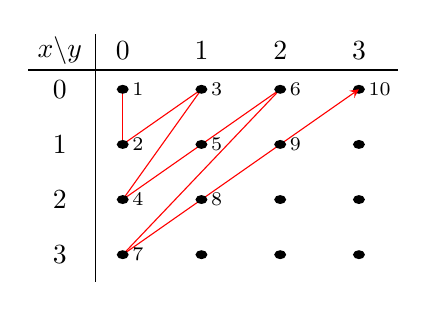
\begin{tikzpicture}[yscale=.7]
			\usetikzlibrary{arrows.meta}
			
			\tikzset{
				myarrow/.style=-stealth
			}
			
			\foreach \x in {0,1,2,3} {
				\node at (.2,-\x-1) {\x};
			}
			\foreach \y in {0,1,2,3} {
				\node at (\y+1,-.3) {\y};
			}
			\draw[red] (1,-1) -- (1,-2);
			\draw[red] (1,-2) -- (2,-1);
			\draw[red] (2,-1) -- (1,-3);
			\draw[red] (1,-3) -- (3,-1);
			\draw[red] (3,-1) -- (1,-4);
			\draw[red] (1,-4) -- (3+.2,-2+.2);
			
			\node at (.2,-.3) {$x\backslash y$};
			\foreach \x in {0,1,2,3} {
				\foreach \y in {0,1,2,3} {
					\ifthenelse{\x<\y \OR \x=\y}{
						\draw[thick,fill] (4-\y,-\x-1) circle (.06);
					}{}
				}
			}
			\draw[myarrow,red] (3+.2,-2+.2) -- (4,-1);
			\node[right] at (1,-1) {\scriptsize 1};
			\node[right] at (1,-2) {\scriptsize 2};
			\node[right] at (2,-1) {\scriptsize 3};
			\node[right] at (1,-3) {\scriptsize 4};
			\node[right] at (2,-2) {\scriptsize 5};
			\node[right] at (3,-1) {\scriptsize 6};
			\node[right] at (1,-4) {\scriptsize 7};
			\node[right] at (2,-3) {\scriptsize 8};
			\node[right] at (3,-2) {\scriptsize 9};
			\node[right] at (4,-1) {\scriptsize 10};
			
			\draw (-.2,-.65) -- (4.5,-.65);
			\draw (.65,0) -- (.65,-4.5);
			
\end{tikzpicture}

	\end{minipage}
\end{center}

Il valore $\langle x,y \rangle$ rappresenta l'incrocio tra la $x$-esima riga e la $y$-esima colonna. Per costruirla:
\begin{enumerate}
	\item $x = 0$
    
	\item si parte dalla cella $(x,0)$ e si enumerano le celle della diagonale identificata da $(x,0)$ e $(0,x)$
	
    \item si incrementa $x$ di $1$ e si ripete dal punto precedente
\end{enumerate}

La funzione e' ovviamente:
\begin{itemize}
	\item iniettiva: non ci possono essere celle con lo stesso numero
	\item suriettiva: ogni numero in $\mathbb{N}^+$ deve comparire
\end{itemize}
Entrambe le proprietà sono soddisfatte, in quanto la numerazione avviene in maniera incrementale, quindi ogni numero prima o poi compare in una cella e di conseguenza ho una coppia che lo genera.

\subsubsection{Forma analitica} 
Per la definizione di $\langle x,y \rangle$ si può notare che
$$ \langle x,y \rangle = \langle x + y,0 \rangle + y $$

\begin{center}
	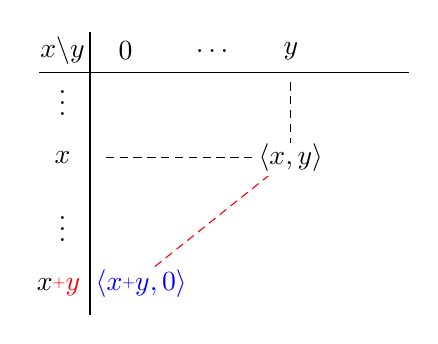
\begin{tikzpicture}[yscale=.8]
		\usetikzlibrary{arrows.meta}
		
		\newcommand{\smallerplus}{\raisebox{.3\height}{\scalebox{.6}{+}}}
		
		\draw[red,densely dashed] (1,-4) -- (3,-2);
		\draw[densely dashed] (.65,-2) -- (3,-2);
		\draw[densely dashed] (3,-1+.2) -- (3,-2);
		
		\node at (.1,-.3) {$x\backslash y$};
		
		\node at (2+1,-.3) {$y$};
		\node at (.9,-.3) {0};
		\node at (1+1,-.3) {$\dots$};
		\node at (.1,-1) {$\vdots$};
		\node at (.1,-1-1) {$x$};
		\node at (.1,-2-1) {$\vdots$};
		\node at (.05,-3-1-.05) {$x{\color{red}\smallerplus y}$};
		\def \offset {.28}
		\draw[white,fill] (3-\offset-.15,-2-\offset) rectangle (3+\offset+.05,-2+\offset-.05);
		\node at (3,-2) {$\langle x,y \rangle$};
		\draw[white,fill] (1-\offset-.15,-4-\offset) rectangle (1+\offset+.05,-4+\offset-.05);
		\node[blue] at (1.1,-4) {$\langle x \smallerplus y, 0 \rangle$};
		
		\draw (-.2,-.65) -- (4.5,-.65);
		\draw (.45,0) -- (.45,-4.5);
\end{tikzpicture}	

\end{center}

Intuitivamente, a partire da $\langle x + y, 0\rangle$ mi basta "salire" seguendo la diagonale fino a $\langle x,y \rangle$, ovvero $y$ posti, e per definizione della funzione, $y$ valori più in alto.

Il calcolo della funzione coppia si può quindi ridurre al calcolo di $\langle x + y, 0 \rangle$. Chiamando $x + y = z$, si può notare come ogni cella
$$ \langle z,0 \rangle = z + \langle z - 1, 0 \rangle $$
E di conseguenza
\begin{align*}
	\langle z,0 \rangle & = z + \langle z - 1, 0 \rangle \\
	& = z + (z-1) + \langle z-2, 0 \rangle \\
	& = z + (z-1) + \dots + 1 + \langle 0,0 \rangle = \\
	& = \left( \sum_{i=1}^{z} i \right) + 1 = \frac{z(z+1)}{2} + 1
\end{align*}

Mettendo insieme le due proprietà viste possiamo ottenere la formula analitica per la funzione coppia: 
$$ \langle x,y \rangle = \langle x + y, 0 \rangle + y = \frac{(x + y) (x + y + 1)}{2} + y + 1 $$

\subsubsection{Forma analitica di $\sin$ e $\des$}

Vogliamo fare la stessa cosa per $\sin$ e $\des$, in modo da poter computare l'inversa della funzione coppia, dato $n$.

Grazie alle osservazioni precedenti sappiamo che
$$ \begin{array}{r c l}
	\gamma = x + y & \implies & x = \gamma + y \\
	n = y + \langle \gamma , 0 \rangle & \implies & y = n - \langle \gamma , 0 \rangle \\
\end{array} $$

Trovando il valore di $\gamma$ possiamo trovare $x$ e $y$. Notiamo come $\gamma$ sia il più grande valore che, quando calcolato sulla prima colonna ($\langle \gamma, 0 \rangle$) non supera $n$, ovvero
$$ \gamma = \max \{z \in \mathbb{N} \mid \langle z, 0 \rangle \leq n \} $$

Intuitivamente, si tratta dell'inizio della diagonale che contiene $n$, è "l'inverso" dell'osservazione fatta in precedenza per la quale $ \langle x,y \rangle = \langle x + y,0 \rangle + y $.

Risolviamo quindi la disequazione
\begin{align*}
	\langle z, 0 \rangle \leq n & \implies \frac{z(z+1)}{2} + 1 \leq n \\
	& \implies z^2 + z - 2n + 2 \leq 0 \\
	& \implies z_{1,2} = \frac{-1 \pm \sqrt{1 + 8n - 8}}{2} \\
	& \implies \frac{-1 - \sqrt{8n - 7}}{2} \leq z \leq \frac{-1 + \sqrt{8n - 7}}{2} 
\end{align*}

Come valore di $\gamma$ scegliamo il massimo nell'intervallo precedente, ovvero:
$$ \gamma = \left\lfloor \frac{-1 + \sqrt{8n - 7}}{2} \right\rfloor $$

E con $\gamma$ noto possiamo definire le funzioni $\sin$ e $\des$ come
$$ 
\begin{array}{r c l}
	\des(n) & = & y = n - \langle \gamma, 0 \rangle = n - \frac{\gamma (\gamma + 1)}{2} - 1 \\
	\sin (n) & = & x = \gamma - y
\end{array}
$$

\begin{theor}
	$\mathbb{N} \times \mathbb{N} \sim \mathbb{N}^+$
\end{theor}
\begin{proof}
	La funzione di Cantor è una funzione biettiva tra l'insieme $\mathbb{N} \times \mathbb{N}$ e l'insieme $\mathbb{N}^+$, quindi i due insiemi sono isomorfi. \\
\end{proof}

Possiamo estendere il risultato all'interno dell'insieme $\mathbb{N}$, ovvero:

\begin{theor}
	$\mathbb{N} \times \mathbb{N} \sim \mathbb{N}$
\end{theor}
\begin{proof}
	Definiamo la funzione 
	$$ [\_ , \_]: \mathbb{N} \times \mathbb{N} \rightarrow \mathbb{N} $$
	tale che
	$$ [x,y] = \langle x,y \rangle - 1$$
	Questa funzione è anch'essa biettiva, quindi i due insiemi sono isomorfi. \\
\end{proof}

Grazie a questo è possibile dimostrare anche che $\mathbb{Q} \sim \mathbb{N}$, infatti i numeri razionali si possono rappresentare come coppie (num, den) e, in generale, tutte le tuple finite sono isomorfe a $\mathbb{N}$, basta iterare in qualche modo la funzione coppia di Cantor.

\subsection{Applicazione alle strutture dati}

I risultati ottenuti fin'ora rendono intuibile come ogni dato possa essere trasformato in un numero, soggetto a trasformazioni matematiche. La dimostrazione \textit{formale} non verrà fatta, anche se verranno fatti esempi di alcune strutture dati che possono essere trasformate in un numero tramite la funzione coppia di Cantor. Ogni struttura dati può essere manipolata e trasformata in una coppia $(x,y)$.

Le \textbf{liste} sono le strutture dati più utilizzate nei programmi. In generale non ne è nota la grandezza, di conseguenza è necessario trovare un modo, soprattutto durante l'applicazione di $\sin$ e $\des$, per capire quando sono finiti gli elementi della lista.

Estendiamo la funzione coppia a una lista di interi $x_1, \dots, x_n$:
$$ \langle x_1, \dots, x_n \rangle \rightarrow \langle x_1, \langle x_2 \langle \dots \langle x_n, 0 \rangle \dots \rangle \rangle \rangle $$

Lo $0$ rappresenta il fine lista e non è necessario nel caso in cui il numero di elementi è noto (array).

La decodifica è il processo inverso, partendo dal numero finale si applicano le funzioni $\sin$ e $\des$ ottenendo a ogni iterazione: 
\begin{itemize}
	\item da $\des$ la somma parziale, su cui riapplicare la funzione per ottenere il valore successivo
	
    \item da $\sin$ il valore presente all'interno della lista
\end{itemize} 

Termina quando il risultato di $\des$ è zero, ovvero l'elemento di fine lista che abbiamo inserito ($x_n$ nel caso di array).
\begin{center}
	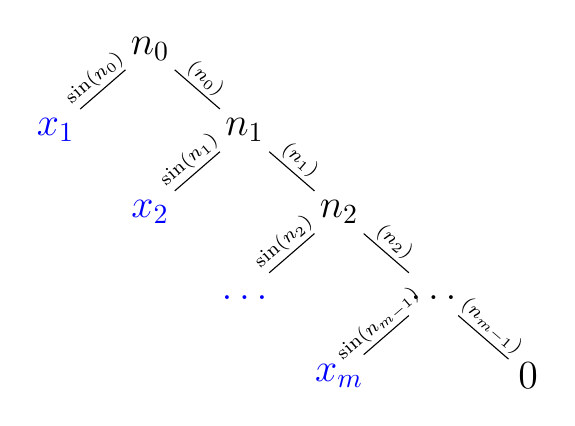
\begin{tikzpicture}[
		level distance=13mm,
		sibling distance=30mm,
		scale=0.8
		]
		\node {\Large$n_0$} 
		child {node[blue] {\Large$x_1$} 
			edge from parent node[xshift=-3,yshift=4,rotate=40.8] {\scriptsize$\sin(n_0)$}
		}
		child {node {\Large$n_1$}
			child {node[blue] {\Large$x_2$}
				edge from parent node[xshift=-3,yshift=4,rotate=40.8] {\scriptsize$\sin(n_1)$}  
			}
			child {node {\Large$n_2$}
				child {node[blue] {\Large$\phantom{n_1}\dots\phantom{n_1}$}
					edge from parent node[xshift=-3,yshift=4,rotate=40.8] {\scriptsize$\sin(n_2)$}  
				}
				child {node {\Large$\phantom{n_1}\dots\phantom{n_1}$}
					child {node[blue] {\Large$x_m$}
						edge from parent node[xshift=-3,yshift=4,rotate=40.8] {\scriptsize$\sin(n_{m-1})$}  
					}
					child {node {\Large$0$} edge from parent 
						node[xshift=3,yshift=4,rotate=-40.8] {\scriptsize$\des(n_{m-1})$}}
					edge from parent node[xshift=3,yshift=4,rotate=-40.8] {\scriptsize$\des(n_2)$}
				}
				edge from parent node[xshift=3,yshift=4,rotate=-40.8] {\scriptsize$\des(n_1)$}
			}
			edge from parent node[xshift=3,yshift=4,rotate=-40.8] {\scriptsize$\des(n_0)$}
		};
\end{tikzpicture}

\end{center}

Se è presente uno 0 all'interno della lista non è un problema in quanto lo 0 compare come risultato di $\des$ solo a fine lista.

%TODO Commento
\lcomment{Qui guarda la lista (ci sono anche degli esercizi qui nelle slide guarda 5:7 in poi)}[-0.15cm]

Quindi è possibile codificare liste e, di conseguenza, \textbf{qualsiasi tipo di dato}, basta convertirlo in una lista di numeri. 

Ad esempio:
\begin{itemize}
	\item una matrice può essere vista come array di array
	
    \item un grafo può essere rappresentato tramite la sua matrice di adiacenza
	
    \item i testi sono liste di caratteri
	
    \item i suoni si possono campionare per ottenere una lista di valori
	
    \item le immagini sono una "matrice" di pixel, ognuno dei quali ha un colore come valore
\end{itemize}

Abbiamo visto come i dati possano essere sostituiti da delle codifiche numeriche; di conseguenza possiamo sostituire tutte le funzioni
$$ f: \dati \rightarrow \dati_{\bot} \;\; \text{ con funzioni } \;\; f': \mathbb{N} \rightarrow \mathbb{N}_\bot $$

In altre parole, l'universo dei problemi per i quali cerchiamo una soluzione automatica è rappresentabile da $\mathbb{N}_\bot^{\mathbb{N}}$.

\section{$\prog \sim \mathbb{N}$}

Adesso lavoriamo sulla parte della relazione che afferma 
$$ F(\C) \sim \prog \sim \mathbb{N} $$

Da notare che la prima parte è più complicata di quanto non sembri, in verità una funzione può avere più programmi associati ma entrambi gli insiemi sono infiniti numerabili, quindi in principio esiste una biezione.

Vogliamo affermare che la potenza computazionale (l'insieme dei programmi che un sistema di calcolo $\C$ riesce a calcolare, $F(\C)$) è isomorfa all'insieme di tutti i programmi, a loro volta isomorfi a $\mathbb{N}$. 

Vogliamo arrivare a ricavare un numero dato un programma e viceversa. Per farlo servirà vedere l'insieme $\prog$ come l'insieme dei programmi scritti in un certo linguaggio di programmazione.

I sistemi analizzati saranno: 
\begin{itemize}
	\item sistema di calcolo $\ram$
    
	\item sistema di calcolo $\while$
\end{itemize}

Il sistema $\ram$ può apparentemente sembrare "troppo semplice", quindi il sistema $\while$ verrà usato per avere un confronto tra le potenze computazionali. \textit{Un sistema più sofisticato porta a poter risolvere più problemi?}

Ci sono due possibili soluzioni: 
\begin{itemize}
	\item $F(\ram) \neq F(\while)$: la computabilità \textit{dipende dal sistema usato}
    
	\item $F(\ram) = F(\while)$: la computabilità è \textit{intrinseca nei problemi} e, di conseguenza, tutti i sistemi sono equivalenti (Tesi di Church-Turing)
\end{itemize}

Il secondo caso è più promettente e, in quel caso, l'obiettivo diventerebbe trovare una \textit{caratterizzazione teorica}, ovvero un "confine" per i problemi calcolabili.

\subsection{Sistema di calcolo $\ram$}

Il sistema di calcolo $\ram$ è un sistema semplice che permette di definire rigorosamente: 
\begin{itemize}
	\item $\prog \sim \mathbb{N}$

	\item la \textbf{semantica} dei programmi eseguibili, ovvero $\C(P,\_)$, con $\C = \ram$, ottenendo $\ram (P,\_)$

	\item la \textbf{potenza computazionale}, ovvero calcolare $F(\C)$ con $\C = \ram$, ottenendo $F(\ram)$
\end{itemize}

\subsubsection{Struttura}

Una macchina $\ram$ è formata da un processore e da una memoria teoricamente infinita, divisa in \textbf{celle/registri} contenenti numeri naturali (dati aritmetizzati).

Indichiamo i \textbf{registri} con $R_k$, con $k \geq 0$. Tra questi 
\begin{itemize}
	\item $R_0$ contiene l'output
    
	\item $R_1$ contiene l'input
\end{itemize}

Inoltre è presente un registro $L$, anche detto \textbf{program counter} $PC$ che indica l'indirizzo dell'istruzione successiva. 

Un \textbf{programma} $P$ è un insieme ordinato di istruzioni, indichiamo con $|P|$ il numero di istruzioni che il programma contiene.

Le \textbf{istruzioni} nel linguaggio RAM sono: 
\begin{itemize}
	\item \textbf{incremento}: $R_k \leftarrow R_k + 1$
	
    \item \textbf{decremento}: $R_k \leftarrow R_k \dotminus 1$
	
    \item \textbf{salto condizionato}: \texttt{if $R_k = 0$ then goto $m$}, con $m \in \{1, \dots, |P|\}$
\end{itemize}
L'istruzione di decremento è tale che
$$ x \dotminus y = \begin{cases}
	x-y & \text{ se } x \geq y\\
	0 & \text{ altrimenti }
\end{cases}$$

\begin{center}
	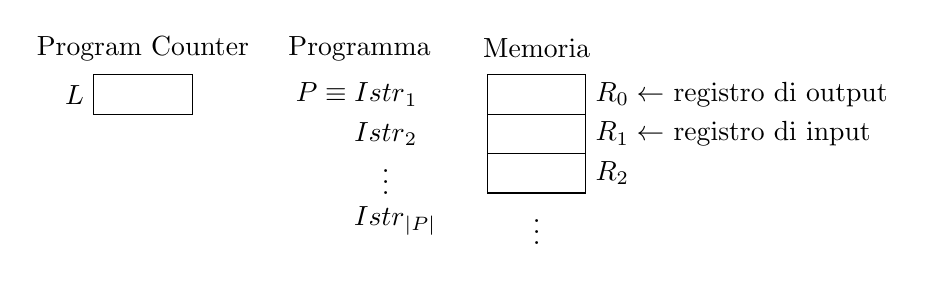
\begin{tikzpicture}
    \node[above] at (.875,.6) {Memoria};

    \draw (.25,0) rectangle (1.5,.5);
    \node[right] at (1.5,.25) {$R_0 \leftarrow$ registro di output};
    \draw (.25,-.5) rectangle (1.5,0);
    \node[right] at (1.5,-.25) {$R_1 \leftarrow$ registro di input};
    \draw (.25,-1) rectangle (1.5,-.5);
    \node[right] at (1.5,-.75) {$R_2$};
    
    \node[below] at (.875,-1) {$\vdots$};

    \def\y{2.25}
    \node[above] at (.875-\y,.55) {Programma};
    \node[] at (.84-\y,.25) {$P\equiv\text{Istr}_1$};
    \node[] at (1.21-\y,-.25) {$\text{Istr}_2$};
    \node[] at (1.21-\y,-.75) {$\vdots$};
    \node[] at (1.33-\y,-1.35) {$\text{Istr}_{|P|}$};

    \def\x{5}
    \node[above] at (.875-\x,.55) {Program Counter};

    \draw (.25-\x,0) rectangle (1.5-\x,.5);
    \node[left] at (1.5-1.25-\x,.25) {$L$};
\end{tikzpicture}

\end{center}

\subsubsection{Esecuzione di un programma RAM}

L'esecuzione di un programma su una macchina RAM segue i passi:
\begin{enumerate}
	\item \textbf{Inizializzazione}:
	\begin{itemize}
		\item viene caricato il programma $P \equiv \text{Istr}_1, \dots \text{Istr}_n$ in memoria
		
        \item il PC viene posto a 1 per indicare di eseguire la prima istruzione del programma
		
        \item viene caricato l'input in $R_1$
		
        \item ogni altro registro è azzerato
	\end{itemize}
	
    \item \textbf{Esecuzione}: le istruzioni vengono eseguite una dopo l'altra, a ogni iterazione passa da $L$ a $L+1$ (escluse operazioni di salto). Essendo il linguaggio RAM \textit{non strutturato} richiede un PC per sapere l'operazione da eseguire al passo successivo.
	
    \item \textbf{Terminazione}: per convenzione, si usa $L = 0$ per indicare che l'esecuzione del programma è terminata o andata in loop. Nel caso in cui il programma termini, è detto \textbf{segnale di halt} e arresta la macchina
	
    \item \textbf{Output}: il contenuto di $R_0$, in caso di halt, contiene il risultato dell'esecuzione del programma $P$. Si indica con $\varphi_P(n)$ il contenuto del registro $R_0$ in caso di halt, oppure $\bot$ in caso di loop
	$$ 
	\varphi_P (n) = \begin{cases}
		cont(R_0) & \text{ se halt} \\
		\bot & \text{ se loop}
	\end{cases}
	$$
\end{enumerate}

Con $\varphi_P: \mathbb{N} \rightarrow \mathbb{N}_\bot$ indichiamo la semantica del programma $P$. Con $\C(P,\_)$ indicavamo la semantica di $P$ nel sistema di calcolo $\C$, quindi con $\ram(P,\_) = \varphi_P$ indichiamo la semantica di $P$ nel sistema di calcolo $\ram$.

\subsubsection{Semantica Operazionale}

Per dare una definizione formale della semantica di un programma $\ram$ va specificato il significato di ogni istruzione (\textbf{semantica operazionale}), esplicitando l'effetto che quell'istruzione ha sui registri della macchina.

Ogni istruzione fa passare la macchina da uno stato all'altro e la \textbf{semantica operazionale} di un'istruzione è la \textbf{coppia} formata dagli \textbf{stati} della macchina \textbf{prima e dopo l'istruzione}.
$$ \text{STATO}_1 \rightarrow \boxed{\text{Istr}_i} \rightarrow \text{STATO}_2 $$

La \textbf{semantica operazionale} di un'istruzione $\text{Istr}_i$ è quindi una \textbf{relazione sui possibili stati}:
$$
\text{Istr}_i \subseteq \text{Stati} \times \text{Stati}
$$

Questa può essere vista come funzione parziale o relazione.

Uno stato deve descrivere completamente la situazione della macchina in un certo istante. Il programma rimane uguale, quindi l'informazione da salvare è la situazione globale dei registri $R_k$ e il registro $L$.

La \textbf{computazione} del programma $P$ è una sequenza di stati $\st_i$, ognuno generato dall'esecuzione di un'istruzione del programma; $P$ induce una sequenza di stati $\st_i$, se questa è formata da un numero infinito di stati, allora il programma è andato in loop; in caso contrario, nel registro $R_0$ si trova il risultato $y$ della computazione di $P$.
$$ 
\varphi_P: \mathbb{N} \rightarrow \mathbb{N}_\bot \tc \varphi_P(n) = \begin{cases}
	y & \text{ se } \exists \st_{fin} \\
	\bot & \text{ altrimenti}
\end{cases}
$$

Quindi, se il programma finisce, la semantica di quest'ultimo è il risultato del programma stesso, ovvero il valore posto nel registro $R_0$ al termine della computazione, $\bot$ altrimenti.

Per definire come passare da uno stato all'altro, definiamo formalmente: 
\begin{itemize}
	\item \textbf{Stato}: istantanea di tutte le componenti della macchina, è una funzione 
	$$ \st: \{L, R_i\} \rightarrow \mathbb{N} $$
	tale che $\st (R_k)$ restituisce il contenuto del registro $R_k$ quando la macchina si trova nello stato $\st$. Gli stati possibili di una macchina appartengono all'insieme 
	$$ \stati = \{f: \{L, R_i\} \rightarrow \mathbb{N}\} = \mathbb{N}^{\{L,R_i\}} $$
	
    Questa rappresentazione permette un numero di registri potenzialmente infinito; se così non fosse, avremmo tuple per indicare tutti i possibili registri al posto dell'insieme $\{L,R_i\}$

	\item \textbf{Stato Finale}: uno stato finale $\st_{fin}$ è un qualsiasi stato $\st$ tale che $\st (L) = 0$
	
    \item \textbf{Dati}: già dimostrato come $\dati \sim \mathbb{N}$
	
    \item \textbf{Inizializzazione}: serve una funzione che, preso l'input, restituisca lo stato iniziale della macchina: 
	$$ \text{in}: \mathbb{N} \rightarrow \stati \tc \text{in}(n) = \st_{init}$$
    
	Lo stato iniziale $\st_{init}$ è tale che
	$$ 
	\st_{init} (R) = \begin{cases}
		1 & \text{ se } R=L \\
		n & \text{ se } R=R_1 \\
		0 & \text{ altrimenti}
	\end{cases}
	$$
    
    Lo stato iniziale è quindi composto da 1 nel $PC$, l'input $n$ in $R_1$, 0 in tutti gli altri registri
	
    \item \textbf{Programmi}: $\prog$ è definito come l'insieme dei programmi $\ram$
\end{itemize}

Manca da definire la \textit{parte dinamica} del programma, ovvero l'esecuzione. Per farlo, definiamo la \textbf{funzione di stato prossimo}: 
$$ \delta : \stati \times \prog \rightarrow \stati_\bot $$
tale che:
$$ \delta (\st,P) = \st' $$
dove $\st$ rappresenta lo stato attuale e $\st'$ rappresenta lo stato prossimo dopo l'esecuzione di un'istruzione di $P$.

La funzione $\delta (\st, P) = \st'$ è tale che
\begin{itemize}
	\item se $\st(L) = 0$ ho halt, ovvero deve terminare la computazione. Poniamo lo stato come indefinito, ovvero $\st' = \bot$
	
    \item Se $\st(L)>|P|$ vuol dire che $P$ non contiene istruzioni che bloccano esplicitamente l'esecuzione del programma. Lo stato $\st'$ è tale che 
	$$ 
	\st'(R) = \begin{cases}
		0 & \text{ se } R = L \\
		\st(R_i) &\text{ se } R = R_i, \forall i
	\end{cases}
	$$
	
    \item Se $1 \leq \st(L) \leq |P|$ considero l'istruzione $\st(L)$-esima:
	\begin{itemize}
		\item se ho un incremento/decremento sul registro $R_k$ definisco $\st'$ tale che 
		$$ 
		\begin{cases}
			\st'(L) & = \st (L) + 1\\
			\st'(R_k) & = \st (R_k) \pm 1\\
			\st'(R_i) & = \st (R_i) \; \text{ per } \; i \neq k \\
		\end{cases}
		$$
	
    	\item Se ho \verb|IF| $R_k = 0$ \verb|THEN GOTO| $m$, definisco $\st'$ tale che
		$$ 
		\st' (L) = \begin{cases}
			m & \text{ se } \st (R_k) = 0 \\
			\st (L) + 1 & \text{ altrimenti}
		\end{cases}
		$$
		$$ \st' (R_i) = \st (R_i), \; \forall i $$
	\end{itemize}
\end{itemize}

L'esecuzione di un programma $P \in \prog$ su input $n \in \mathbb{N}$ genera una sequenza di stati
$$ \st_0, \st_1, \dots, \st_i, \st_{i+1}, \dots $$
tali che:
$$
\begin{array}{l l c l}
	& \st_0 & = & \text{in}(n) \\
	\forall i & \st_{i+1} & = & \delta (\st_i,P) 
\end{array}
$$

La sequenza è infinita quando $P$ va in loop, mentre se termina raggiunge uno stato $\st_m$ tale che $\st_m (L) = 0$, ovvero ha ricevuto il segnale di halt.

La semantica di $P$ è
$$ 
\varphi_P (n) = \begin{cases}
	y & \text{ se } P \text{ termina in } \st_m, \text{ con } \st_m (L) = 0 \text{ e } \st_m(R_0) = y \\
	\bot & \text{ se } $P$ \text{ va in loop}
\end{cases}
$$

La potenza computazionale del sistema $\ram$ è 
$$ F(\ram) = \left\{f \in \mathbb{N}^{\mathbb{N}}_\bot \ | \ \exists P \in \prog \text{ s.t. } \varphi_P = f \right\} = \left\{\varphi_P \ | \ P \in \prog \right\} \subsetneq \mathbb{N}^{\mathbb{N}}_\bot $$
L'insieme è formato da tutte le funzioni $f: \mathbb{N} \rightarrow \mathbb{N}_\bot$ che hanno un programma che le calcola in un sistema $\ram$. \lcomment{Guarda slide per esempi esercizi 6:10 in poi} % TODO Commento

\subsection{Aritmetizzazione di un programma}

Per verificare che $\prog \sim \mathbb{N}$ basterebbe trovare una funzione che permetta di codificare i programmi in numeri in modo biunivoco. Data una lista di istruzioni semplici $P \equiv \text{Istr}_1, \dots, \text{Istr}_m$ se questa fosse codificata come una lista di interi potremmo sfruttare la funzione coppia di Cantor per ottenere un numero associato al programma $P$. Quindi vogliamo trovare una funzione $Ar$ che associ a ogni istruzione $I_k$ la sua codifica numerica $c_k$. Se la funzione trovata è anche biunivoca siamo sicuri di poter trovare anche la sua inversa, ovvero la funzione che ci permette di ricavare $I_k$ da $c_k$.

Riassumendo, vogliamo trasformare la lista di istruzioni un una lista di numeri su cui successivamente applicare la funzione coppia di Cantor. Vorremmo anche ottenere la lista di istruzioni originale data la codifica.
\begin{center}
	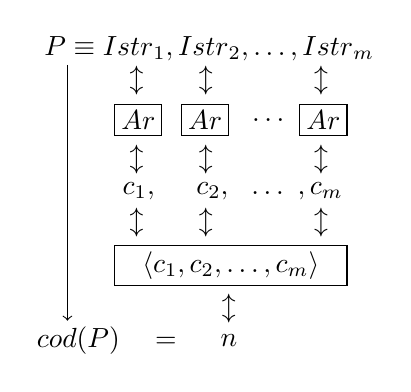
\begin{tikzpicture}
    \node at (0,0)
        {$ P \equiv \text{Istr}_1,\text{Istr}_2,\dots,\text{Istr}_m$};
    \node at (.25,-.4) 
        {$\updownarrow \qquad \updownarrow \qquad \ \ \ \ \ \updownarrow$};
    
    \draw (-1.2,-1.1) rectangle (-.6,-.7) node[midway] {$Ar$};
    \begin{scope}[xshift=.85cm]
        \draw (-1.2,-1.1) rectangle (-.6,-.7) node[midway] {$Ar$};
    \end{scope}
    \begin{scope}[xshift=2.35cm]
        \draw (-1.2,-1.1) rectangle (-.6,-.7) node[midway] {$Ar$};
    \end{scope}
    \node at (.75,-.9) {$\dots$};

    \node at (.25,-1.4) 
        {$\updownarrow \qquad \updownarrow \qquad \ \ \ \ \ \updownarrow$};
    \node at (.3,-1.8) 
        {$c_1,\ \ \ \ c_2, \ \ \dots \  ,c_m$};
    \node at (.25,-2.2) 
        {$\updownarrow \qquad \updownarrow \qquad \ \ \ \ \ \updownarrow$};
    \draw (-1.2,-3) rectangle (1.75,-2.5) node[midway] 
        {$\langle c_1,c_2,\dots,c_m \rangle$};
    \node at (.25,-3.3) {$\updownarrow$};
    \node at (.25,-3.7) {$n$};
    \node at (-1.3,-3.7) {$cod(P) \quad =$};
    \draw [->] (-1.8,-.2) -- (-1.8,-3.45);

\end{tikzpicture}

\end{center} 

L'associazione biunivoca di un numero a una struttura si dice aritmetizzazione o G\"odelizzazione.

\subsubsection{Applicazione ai programmi RAM}

Dovendo codificare tre istruzioni nel linguaggio $\ram$, definiamo la funzione $Ar$ tale che
$$ 
Ar(I) = \begin{cases}
	3k & \text{ se } I \equiv R_k \leftarrow R_k + 1 \\
	3k + 1 & \text{ se } I \equiv R_k \leftarrow R_k \dotminus 1 \\
	3 \langle k,m\rangle - 1 & \text{ se } I \equiv \text{ \texttt{if} } R_k = 0 \text{ \texttt{then goto} } m \\
\end{cases}
$$

Per l'inversa, in base al modulo tra $n$ e 3 ottengo una certa istruzione: 
$$
Ar^{-1} (n) = \begin{cases}
	R_{\frac{n}{3}} \leftarrow R_{\frac{n}{3}} + 1 & \text{ se } n \mod 3 = 0 \\
	R_{\frac{n-1}{3}} \leftarrow R_{\frac{n-1}{3}} \dotminus 1 & \text{ se } n \mod 3 = 1 \\
	\text{\texttt{if} } R_{\sin\left(\frac{n+1}{3}\right)} = 0 \text{ \texttt{then goto} } \des\left(\frac{n+1}{3}\right) & \text{ se } n \mod 3 = 2 \\
\end{cases}
$$

Per tornare indietro devo prima invertire la funzione coppia di Cantor e poi invertire la funzione $Ar$.
La lunghezza del programma $P$, indicata con $|P|$, si calcola come $len(cod(P))$. Abbiamo quindi dimostrato che $\prog \sim \mathbb{N}$. \lcomment{Guarda le prime slide fino a 7:5 per esempi} % TODO Commento

\subsubsection{Osservazioni}
Avendo $n = cod(P)$ si può scrivere
$$ \varphi_P (t) = \varphi_n (t) $$
Ovvero, la semantica di $P$ è uguale alla semantica della sua codifica. I numeri diventano un \textit{linguaggio di programmazione}.

Si può scrivere l'insieme 
$$ F(\ram) = \{\varphi_P: P \in \prog \}$$
come 
$$ F(\ram) = \{\varphi_i\}_{i \in \mathbb{N}} $$
L'insieme, grazie alla dimostrazione di $\prog \sim \mathbb{N}$, è numerabile. Abbiamo dimostrato rigorosamente che:
$$ F(\ram) \sim \mathbb{N} \nsim \mathbb{N}^{\mathbb{N}}_\bot $$
Di conseguenza, anche nel sistema di calcolo $\ram$ esistono funzioni non calcolabili.

La $\ram$ è troppo elementare affinché $F(\ram)$ rappresenti formalmente la "classe dei problemi risolubili automaticamente", quindi considerando un sistema di calcolo $\C$ più sofisticato, ma comunque trattabile rigorosamente come il sistema $\ram$, potremmo dare un'idea formale di "ciò che è calcolabile automaticamente". 

Riuscendo a dimostrare che $F(\ram) = F(\C)$ allora cambiare la tecnologia non cambia ciò che è calcolabile, la calcolabilità è intrinseca ai problemi e la si può caratterizzare matematicamente.

\subsection{Sistema di calcolo $\while$}

Introduciamo quindi il sistema di calcolo $\while$ per vedere se riusciamo a "catturare" più o meno funzioni calcolabili dalla macchina $\ram$.

\subsubsection{Struttura}

La macchina $\while$ ha anch'essa, come la macchina $\ram$, una serie di registri, ma al posto di essere \textit{potenzialmente infiniti} sono esattamente 21. 

Il registro $R_0$ è il \textbf{registro di output}, mentre $R_1$ è il \textbf{registro di input}. Non esiste il Program Counter in quanto il linguaggio è \textbf{strutturato} e ogni istruzione in questo linguaggio va eseguita in ordine.

Il linguaggio $\while$ prevede una \textbf{definizione induttiva}: vengono definiti alcuni comandi base e i comandi più complessi sono una concatenazione dei comandi base.

\paragraph{Assegnamento:} Comando di base, ne esistono di tre tipi:
\begin{align*}
	x_k & := 0, \\
	x_k & := x_j + 1 \\
	x_k & := x_j \dotminus 1
\end{align*}

Queste istruzioni sono più complete rispetto alle istruzioni $\ram$, in una sola istruzione si può azzerare il valore di una variabile o assegnare a una variabile il valore di un'altra aumentato/diminuito di 1.

\paragraph{While:} Primo comando "induttivo". Si tratta di un comando della forma: 
\begin{center}
	\texttt{while} $x_k \neq 0$ \texttt{do} $C$
\end{center}

Dove $C$ è detto \textbf{corpo} e può essere un assegnamento, un comando while o un comando composto.

\paragraph{Composto:} Altro comando induttivo. Si tratta di un comando nella forma
\begin{center}
	\texttt{begin} $C_1; \dots; C_n$ \texttt{end}
\end{center}

Dove i vari $C_i$ sono, come prima, assegnamenti, comandi while o comandi composti.

\paragraph{Programma $\while$:} Un programma $\while$ è un comando composto, e l'insieme di tutti i programmi $\while$ è l'insieme
$$ W\text{-}\prog = \{\prog \text{ scritti in linguaggio } \while \} \lcomment{Guarda le slide ci sono degli esempi} $$

Chiamiamo
$$ \Psi_W : \mathbb{N} \rightarrow \mathbb{N}_\bot $$
la \textbf{semantica} del programma $W \in W-\prog$.

Per dimostrare una proprietà $P$ di un programma $W \in \wprog$, data la definizione induttiva del linguaggio $\while$, è naturale procedere induttivamente:
\begin{enumerate}
	\item dimostro $P$ vera sugli assegnamenti 
	
    \item suppongo $P$ vera sul comando $C$ e la dimostro vera per \texttt{while $x_k \neq 0$ do $C$}
	
    \item suppongo $P$ vera sui comandi $C_1, \dots, C_n$ e la dimostro vera per \texttt{begin $C_1; \dots; C_n$ end}
\end{enumerate}

\subsubsection{Esecuzione di un programma $\while$}

L'esecuzione di un programma $\while$ $W$ è composta dalle seguenti fasi: 
\begin{enumerate}
	\item \textbf{Inizializzazione}: ogni registro $x_i$ viene posto a $0$, tranne $x_1$, che contiene l'input $n$
    
	\item \textbf{Esecuzione}: essendo $\while$ un linguaggio con strutture di controllo, non serve un Program Counter, poiché le istruzioni di $W$ vengono eseguite l'una dopo l'altra
	
    \item \textbf{Terminazione}: l'esecuzione di $W$ può 
	\begin{itemize}
		\item \textit{arrestarsi}: se arriva al termine delle istruzioni
	
    	\item \textit{non arrestarsi}: se entra in un loop
	\end{itemize}
	
    \item \textbf{Output}: Se il programma va in halt, l'output è contenuto nel registro $x_0$. Possiamo scrivere
	$$ \Psi_W (n) = \begin{cases}
		cont(x_0) & \text{ se halt} \\
		\bot & \text{ se loop}
	\end{cases}$$
    La semantica del programma, ancora una volta, coincide con il valore di output, questa volta contenuto all'interno di $x_0$, $\bot$ se non termina
\end{enumerate}

\subsubsection{Definizione formale per l'esecuzione}

Come per i programmi $\ram$, serve una definizione formale per la semantica di un programma $\while$, per la quale servono una serie di elementi
\begin{itemize}
	\item \textbf{Stato}: una tupla grande quanto il numero di variabili, dove quindi $\underline{x} = (c_0, \dots, c_{20})$ rappresenta uno stato, con $c_i$ rappresentante il contenuto della variabile $i$
	
    \item \textbf{$\wstati$}: Insieme di tutti gli stati possibili, contenuto in $\mathbb{N}^{21}$ vista la definizione degli stati 
	
    \item \textbf{Dati}: già visto che $\dati \sim \mathbb{N}$
	
    \item \textbf{Inizializzazione}: Lo stato iniziale è descritto dalla funzione 
	$$ w\text{-}in(n) = (0, n, 0, \dots, 0) $$
	
    \item \textbf{Semantica operazionale}: Vogliamo trovare una funzione che, presi comando da eseguire e stato corrente, restituisce lo stato successivo
\end{itemize}

\paragraph{Funzione stato prossimo:} Soffermandoci sull'ultimo punto, vogliamo trovare la funzione
$$  \llbracket \_ \rrbracket ( \_ ): \wcom \times \wstati \rightarrow \wstati_\bot $$
Che, dati un comando $C$ del linguaggio $\while$ e lo stato corrente $\underline{x}$, calcoli:
$$ \llbracket C \rrbracket (\underline{x}) = \underline{y} $$
con $\underline{y}$ stato prossimo. Quest'ultimo dipende dal comando $C$, ma essendo $C$ induttivo, possiamo provare a dare una definizione induttiva della funzione.

Partendo dal passo base, gli \textbf{assegnamenti}:
$$
\llbracket x_k := 0 \rrbracket (\underline{x}) = \underline{y} = \begin{cases}
	x_i & \text{ se } i \neq k \\
	0 & \text{ se } i = k
\end{cases}
$$
$$ 
\llbracket x_k := x_j \pm 1 \rrbracket (\underline{x}) = \underline{y} = \begin{cases}
	x_i & \text{ se } i \neq k \\
	x_j \pm 1 & \text{ se } i = k
\end{cases}
$$

Proseguiamo con il \textbf{passo induttivo}:
\begin{itemize}
	\item \textbf{Comando composto}: vogliamo calcolare
	$$ \llbracket \text{\texttt{begin }} C_1; \dots; C_n \text{\texttt{ end}} \rrbracket (\underline{x}) $$
	
    Conoscendo ogni $\llbracket C_i \rrbracket$ per ipotesi induttiva, calcoliamo la funzione
	$$ \llbracket C_n \rrbracket \left(\dots \left(\llbracket C_2 \rrbracket \left(\llbracket C_1 \rrbracket (\underline{x})\right)\right) \dots \right) = \left(\llbracket C_n \rrbracket \circ \dots \circ \llbracket C_1 \rrbracket \right) (\underline{x}) $$
	
    Ovvero, applichiamo in ordine i comandi $C_i$ presenti nel comando composto $C$
	
	\item \textbf{Comando while}: vogliamo calcolare
	$$ \llbracket \text{\texttt{while }} x_k \neq 0 \text{ \texttt{do} } C \rrbracket (\underline{x}) $$
	
    Conoscendo $\llbracket C \rrbracket$ per ipotesi induttiva, calcoliamo la funzione
	$$ \llbracket C \rrbracket \left(\dots \left(\llbracket C \rrbracket (\underline{x})\right) \dots \right) $$
	
    Bisogna capire quante volte eseguire il ciclo: dato $\llbracket C \rrbracket^e$ (comando $C$ eseguito $e$ volte) vorremmo trovare il valore di $e$. Questo è il numero minimo di iterazioni che portano in uno stato in cui $x_k = 0$, ovvero il comando \texttt{while} diventa
	$$ \llbracket \text{\texttt{while} } x_k \neq 0 \text{ \texttt{do} } C \rrbracket (\underline{x}) = \begin{cases}
		\llbracket C \rrbracket^e (\underline{x}) & \text{ se } \exists e \text{ minimo tale che } \llbracket C \rrbracket^e (\underline{x})[k] = 0 \\
		\bot & \text{ altrimenti}
	\end{cases}$$
\end{itemize}

Definita la semantica operazionale, manca solo da definire cos'è la \textbf{semantica del programma} $W$ su input $n$. Questa è la funzione
$$ \Psi_W: \N \rightarrow \mathbb{N}_\bot \mid \Psi_W (n) = \text{Pro}\left(0, \llbracket W \rrbracket (w\text{-}in(n))\right) \lcomment{bisognerebbe fare funzione a tratti contando anche il caso $\bot$} $$

Questo è valido in quanto $W$ programma $\while$ è un programma composto, e abbiamo definito come deve comportarsi la funzione $\llbracket \_ \rrbracket (\_)$ sui comandi composti.

Stiamo praticamente dicendo che la semantica del programma $W$, visto come comando composto, è il risultato, ovvero il contenuto del registro $x_0$, dell'applicazione del comando $W$ allo stato iniziale.

\paragraph{Potenza Computazionale:} La potenza computazionale del sistema di calcolo $\while$ è l'insieme 
$$ F(\while) = \left\{f \in \mathbb{N}^{\mathbb{N}}_\bot \mid  \exists W \in \wprog , f = \Psi_W \right\} = \left\{\Psi_W : W \in \wprog \right\}$$

Ovvero, l'insieme formato da tutte le funzioni che possono essere calcolate con un programma in $\wprog$.

\subsection{Confronto tra macchina $\ram$ e $\while$}

Viene naturale confrontare i due sistemi presentati per capire il "\textit{più potente}", sempre che ce ne sia uno. Le possibilità sono: 
\begin{itemize}
	\item $F(\ram) \subsetneq F(\while)$, sarebbe anche comprensibile data l'estrema semplicità del sistema $\ram$
	
    \item $F(\ram) \cap F(\while) = \emptyset$, avere insiemi disgiunti significherebbe che il concetto di calcolabile dipende dalla macchina considerata
	
    \item $F(\while) \subseteq F(\ram)$, che sarebbe sorprendente vista l'apparente maggiore sofisticatezza del sistema $\while$
	
    \item $F(\while) = F(\ram)$, ovvero il concetto di calcolabile non dipende dalla tecnologia utilizzata ma è intrinseco nei problemi
\end{itemize}

\paragraph{Confronto tra sistemi di calcolo:} Ponendo di avere $\C_1$ e $\C_2$ sistemi di calcolo con programmi in $\cprog{1}$ e $\cprog{2}$ e le relative potenze computazionali
$$ F(\C_1) = \left\{f: \mathbb{N} \rightarrow \mathbb{N}_\bot \mid \exists P_1 \in \cprog{1} \mid f = \Psi_{P_1} \right\} = \left\{\Psi_{P_1}: P_1 \in \cprog{1} \right\} $$
$$ F(\C_2) = \left\{f: \mathbb{N} \rightarrow \mathbb{N}_\bot \mid \exists P_2 \in \cprog{2} \mid f = \varphi_{P_2} \right\} = \left\{\varphi_{P_2}: P_2 \in \cprog{2} \right\} $$

Mostrare che il primo sistema non è più potente del secondo $F(\C_1) \subseteq F(\C_2)$ vuol dire dimostrare che ogni elemento nel primo insieme deve stare anche nel secondo
$$ \forall f \in F(\C_1) \implies f \in F(C_2) $$

\textit{Espandendo} la definizione di $f \in F(\C)$ la relazione diventa
$$ \forall P_1 \in \cprog{1} \mid f = \Psi_{P_1} \implies \exists P_2 \in \cprog{2} \mid f = \varphi_{P_2} $$

Per ogni programma calcolabile nel primo sistema di calcolo ne esiste uno con la stessa semantica nel secondo sistema. Vogliamo trovare un \textbf{compilatore} (o \textbf{traduttore}), ovvero una funzione che trasformi un programma del primo sistema in uno del secondo.

\subsubsection{Traduzioni}
Dati $\C_1$ e $\C_2$ due sistemi di calcolo, definiamo \textbf{traduzione} da $\C_1$ a $\C_2$ una funzione
$$ T: \cprog{1} \rightarrow \cprog{2} $$

Con le seguenti proprietà:
\begin{itemize}
	\item \textbf{programmabile}: esiste un modo per programmarla effettivamente

	\item \textbf{completa}: deve saper tradurre \textit{ogni} programma in $\cprog{1}$ in un programma in $\cprog{2}$

	\item \textbf{corretta}: mantiene la semantica dei programmi di partenza, ovvero
	$$ \forall P \in \cprog{1}, \;\; \Psi_P = \varphi_{T(P)}$$
	dove $\Psi$ rappresenta la semantica dei programmi in $\cprog{1}$ e $\varphi$ rappresenta la semantica dei programmi in $\cprog{2}$ \\
\end{itemize}

\begin{theor}
	Se esiste $T: \cprog{1} \rightarrow \cprog{2}$ allora $F(\C_1) \subseteq F(\C_2)$
\end{theor}
\begin{proof}
	Se $f \in F(\C_1)$ allora esiste un programma $P_1 \in \cprog{1}$ tale che $\Psi_{P_1} = f$.
	A questo programma $P_1$ applico $T$, ottenendo $T(P_1) = P_2 \in \cprog{2}$ (per \textit{completezza}) tale che $\varphi_{P_2} = \Psi_{P_1} = f$ (per \textit{correttezza}).
	
	Ho trovato un programma $P_2 \in \cprog{2}$ la cui semantica è $f$, allora $F(\C_1) \subseteq F(\C_2)$.\\
\end{proof}

Mostreremo che $F(\while) \subseteq F(\ram)$, ovvero che il sistema $\while$ non è più potente del sistema $\ram$.

Costruiremo un compilatore
$$ \comp: \wprog \rightarrow \prog $$
che rispetti le caratteristiche di programmabilità, completezza e correttezza.

\subsection{$F(\while) \subseteq F(\ram)$}

Per provare che $F(\while) \subseteq F(\ram)$ vogliamo costruire un compilatore da $\while$ a $\ram$.

Per comodità, introduciamo un linguaggio $\ram$ \textit{etichettato}: aggiunge la possibilità di etichettare un'istruzione che indica un punto di salto o di arrivo (stile label assembly). Non altera la potenza espressiva del linguaggio in quanto si tratta di un'aggiunta puramente sintattica: il $\ram$ etichettato si traduce facilmente in $\ram$ puro.

Essendo $\wprog$ un insieme definito induttivamente, possiamo definire induttivamente anche il compilatore:
\begin{itemize}
	\item \textbf{Passo base}: come compilare gli assegnamenti
	
    \item \textbf{Passo induttivo}:
	\begin{enumerate}
		\item Per I.H., assumo di sapere $\comp(C_1), \dots, \comp(C_m)$ e mostro come compilare il comando composto \texttt{begin $C_1; \dots; C:n$ end}
	
    	\item Per I.H., assumo di sapere $\comp(C)$ e mostro come compilare il comando \texttt{while $x_k \neq 0$ do $C$}
	\end{enumerate}
\end{itemize}

Nelle traduzioni andremo a mappare la variabile $\while$ $x_k$ nel registro $\ram$ $R_k$. Questo non crea problemi in quanto stiamo mappando un numero finito di registri in un insieme infinito.

Il primo assegnamento che mappiamo è $x_k := 0$
\begin{center}
	\renewcommand{\arraystretch}{1.25}
	\begin{tabular}{l|r l|}
		\cline{2-3}
		$\comp(x_k:=0) =$ & \texttt{LOOP}:& \texttt{IF $R_k = 0$ THEN GOTO EXIT}\\
		&& $R_k\leftarrow R_k \dotminus 1$ \\
		&& \texttt{IF $R_{21} = 0$ THEN GOTO LOOP} \\
		&\texttt{EXIT}:& $R_k \leftarrow R_k \dotminus 1$ \\
		\cline{2-3}
	\end{tabular}\vspace{.15cm}
\end{center}

Questo programma $\ram$ azzera il valore di $R_k$ usando il registro $R_{21}$ per saltare al check della condizione iniziale. Viene utilizzato il registro $R_{21}$ perché, non essendo mappato a nessuna variabile $\while$, sarà sempre nullo dopo la fase di inizializzazione.

Gli altri due assegnamenti da mappare sono $x_k:= x_j+1$ e $x_k := x_j \dotminus 1$:
\begin{itemize}
	\item Se $k=j$, la traduzione è banale e l'istruzione $\ram$ è
	$$ \comp(x_k := x_k \pm 1) = R_k \leftarrow R_k \pm 1 $$ \vspace{-0.75cm}
	\item Invece se $k \neq j$ la prima idea è quella di "spostare" $x_j$ in $x_k$ e poi fare $\pm 1$ ma non funziona per due ragioni
	\begin{enumerate}
		\item se $R_k \neq 0$ la migrazione (quindi sommare $R_j$ a $R_k$) non genera $R_j$ dentro $R_k$. Si può risolvere azzerando il registro $R_k$ prima della migrazione
		\item $R_j$ dopo il trasferimento è ridotto a 0, ma questo non è il senso dell'istruzione, vorrei solo "\textit{fotocopiarlo}" dentro $R_k$. Questo può essere risolto salvando $R_j$ in un altro registro, azzerare $R_k$, spostare $R_j$ e ripristinare il valore originale di $R_j$
	\end{enumerate}
%	Ricapitolando: 
%	\begin{itemize}
%		\item salviamo $x_j$ in $R_{22}$, registro \textit{sicuro} perché mai coinvolto in altre istruzioni
%		\item azzeriamo $R_k$
%		\item Rigeneriamo $R_j$ e settiamo $R_k$ da $R_{22}$
%		\item $\pm 1$ in $R_k$
%	\end{itemize}
	Quindi possiamo mappare come:
	\begin{center}
		\renewcommand{\arraystretch}{1.25}
		\begin{tabular}{l|r l|l}\cline{2-3}
			$\comp (x_k := x_j \pm 1)$ = & \texttt{LOOP}:& \texttt{IF $R_j = 0$ THEN GOTO E1}
			&\multirow{4}{*}{\hspace{-.2cm}
				$\begin{rcases}
					\phantom{}\\
					\phantom{}\\
					\phantom{}\\
					\phantom{}\\
				\end{rcases}$ Salva $R_j$ in $R_{22}$
			} \\
			&& $R_j\leftarrow R_j \dotminus 1$ & \\
			&& $R_{22} \leftarrow R_{22} + 1$ & \\
			&& \texttt{IF $R_{21} = 0$ THEN GOTO LOOP} & \\
			& \texttt{E1:} & \texttt{IF $R_k = 0$ THEN GOTO E2} &\multirow{3}{*}{\hspace{-.2cm}
				$\begin{rcases}
					\phantom{}\\
					\phantom{}\\
					\phantom{}\\
				\end{rcases}$ Azzera $R_k$
				}\\
			&& $R_k \leftarrow R_k \dotminus 1$ & \\
			&& \texttt{IF $R_{21} = 0$ THEN GOTO E1} & \\
			& \texttt{E2:} & \texttt{IF $R_{22} = 0$ THEN GOTO E3} & \multirow{4}{*}{\hspace{-.2cm}
			$\begin{rcases}
				\phantom{}\\
				\phantom{}\\
				\phantom{}\\
				\phantom{}\\
				\phantom{}\\
			\end{rcases}$ Rigenera $R_j$ e $R_k$ da $R_{22}$
			} \\
			&& $R_k \leftarrow R_k + 1$ & \\
			&& $R_j \leftarrow R_j + 1$ & \\
			&& $R_{22} \leftarrow R_{22} \dotminus 1$ & \\
			&& \texttt{IF $R_{21} = 0$ THEN GOTO E2} & \\ 
			& \texttt{E3:} & $R_k \leftarrow R_k \pm 1$ & \\
			\cline{2-3} 
		\end{tabular}\vspace{.5cm}
	\end{center}
\end{itemize}

Per I.H. sappiamo come compilare $C_1, \dots C_m$. Possiamo calcolare la compilazione del comando composto come
\begin{center}
	\begin{tabular}{r |l|}
		\cline{2-2}
		$\comp($\texttt{begin $C_1; \dots; C_n$ end$)$} = & $\comp (C_1)$ \\
		& $\dots$ \\
		& $\comp(C_m)$ \\
		\cline{2-2}
	\end{tabular}
\end{center}

Per I.H. sappiamo come compilare $C$. Possiamo calcolare la compilazione del comando \texttt{while} come
\begin{center}
	\begin{tabular}{l |r l|}
		\cline{2-3} 
		$\comp(\text{\texttt{while }} x_k \neq 0 \texttt{ do } C) = $ & \texttt{LOOP:} & \texttt{IF $R_k = 0$ THEN GOTO EXIT} \\
		&& $\comp(C)$ \\
		&& \texttt{IF $R_{21} = 0$ THEN GOTO LOOP} \\
		& \texttt{EXIT:} & $R_k \leftarrow R_k \dotminus 1$ \lcomment{Questa istruzione e' un po come un \texttt{pass}/\texttt{nop} in quanto $R_{k}$ è sicuramente 0} \\
		\cline{2-3}
	\end{tabular}
\end{center}

La funzione
$$ \comp: \wprog \rightarrow \prog $$
appena costruita soddisfa le tre proprietà desiderate in quanto:
\begin{itemize}
	\item Facilmente programmabile
    
	\item Compila ogni Sorgente $\wprog$
	
    \item Mantiene la semantica ovvero $\Psi_P = \varphi_{\comp(P)}$
\end{itemize}

Di conseguenza
$$ F(\while) \subseteq F (\ram) $$

\paragraph{TL;DR:} Vogliamo definire induttivamente un compilatore, definendo prima come compilare gli assegnamenti, poi i comandi composti: 
\begin{itemize}
    \item Per mappare $x_k := 0$, usiamo un loop per decrementare di 1 $R_k$ finché non raggiunge 0 (usando $R_{21}$, sempre posto a 0, per saltare alla condizione iniziale)
    
    \item Per mappare $x_k := x_j \pm 1$
    \begin{itemize}
        \item Se $k = j$ uso banalmente l'incremento/decremento $\ram$
        
        \item Se $k \neq j$, salvo $R_j$ in $R_{22}$ (decrementando uno e incrementando l'altro finché $R_j \neq 0$), azzero $R_k$ (loop che decrementa), rigenero $R_j$ e $R_k$ da $R_{22}$, prima di uscire incremento/decremento di 1 $R_k$
    \end{itemize}
    
    \item Il comando composto è una composizione, che sappiamo essere compilabile per I.H.
    
    \item Il comando \texttt{while} lo possiamo modellare come un loop sulla compilazione del comando all'interno, compilabile per I.H.
\end{itemize}

In questo modo abbiamo una funzione, programmabile, completa e corretta, dimostrando che $F(\while) \subseteq F(\ram)$.

\subsection{$F(\ram) \subseteq F(\while)$}

Abbiamo mostrato che una macchina $\while$ non è più potente di una macchina $\ram$, ora vogliamo fare l'inverso. Per farlo si userà il concetto di interprete.

\subsubsection{Interprete in $\while$ per $\ram$}

Introduciamo il concetto di \textbf{interprete}. Chiamiamo $I_W$ l'interprete scritto in linguaggio $\while$ per programmi scritti in linguaggio $\ram$.

$I_W$ prende in input un programma $P \in \prog$ e un dato $x \in \mathbb{N}$ e restituisce "\textit{l'esecuzione}" di $P$ sull'input $x$. Più formalmente, restituisce la semantica di $P$ su $x$, quindi $\varphi_P (x)$.

\begin{center}
	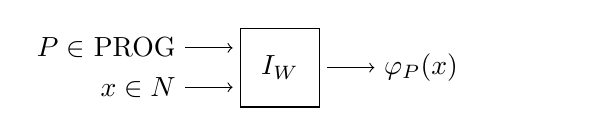
\begin{tikzpicture}
	
	\draw[->] (2.3,1.75) node[left]{$P\in\ $PROG} -- (2.9,1.75);
	\draw[->] (2.3,1.25) node[left]{$x\in \mathbb{N}$} -- (2.9,1.25);
	\draw (3,2) rectangle (4,1);
	\node at (3.5,1.5) {$I_W$};
	\draw[->] (4.1,1.5) -- (4.7,1.5)
	node [right] {$\varphi_P(x)$};
	\node[right] at (4.7,1.5) {$\phantom{\varphi_n(x)=\varphi_P(x)}$};
	
\end{tikzpicture}
\end{center}

Notiamo come l'interprete non crei dei prodotti intermedi, ma si limita a eseguire $P$ sull'input $x$.

Due problemi principali: 
\begin{enumerate}
	\item Il primo riguarda il tipo di input della macchina $\while$ in quanto questa non sa leggere il programma $P$ (listato di istruzioni $\ram$), sa leggere solo numeri. Dobbiamo modificare $I_W$ in modo che non passi più $P$ ma la sua codifica $cod(P) = n \in \mathbb{N}$. Questo restituisce la semantica del programma codificato con $n$, che è $P$, quindi $\varphi_n (x) = \varphi_P (x)$
	
    \item Il secondo problema riguarda la quantità di dati in input alla macchina $\while$: questa legge l'input da un singolo registro, mentre qui ne stiamo passando due. Bisogna modificare $I_W$, condensando l'input tramite la funzione coppia di Cantor, che diventa $\langle x,n \rangle$
\end{enumerate}

Quindi
\begin{center}
	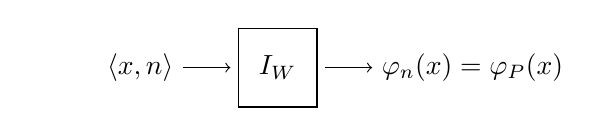
\begin{tikzpicture}
	
	\draw[->] (2.3,1.5) node[left]{$\langle x,n \rangle$} -- (2.9,1.5);
	\node[left] at (2.3,1.5) {$\phantom{cod(P)=n}$};
	\draw (3,2) rectangle (4,1);
	\node at (3.5,1.5) {$I_W$};
	\draw[->] (4.1,1.5) -- (4.7,1.5)
	node [right] {$\varphi_n(x)=\varphi_P(x)$};
	
\end{tikzpicture}
\end{center}

La semantica di $I_W$ diventa
$$ \forall x,n \in \mathbb{N} \;\;\;\; \Psi_{I_W} \left(\langle x,n \rangle \right) = \varphi_n (x) = \varphi_P (x) $$

Similmente a prima, useremo per comodità il linguaggio \textbf{macro-$\while$}, che include alcune macro comode nella scrittura di $I_W$. Viene modificata solo la sintassi e di conseguenza non la potenza del linguaggio.

Le \textbf{macro} utilizzate sono: 
\begin{itemize}
	\item $x_k := x_j + x_s$
	
    \item $x_k := \langle x_j, x_s \rangle$
	
    \item $x_k := \langle x_1, \dots, x_n \rangle$
	
    \item $x_k := \proj(x_j, x_s)$, proiezione, estrae l'elemento $x_j$-esimo dalla lista codificata in $x_s$
	
    \item $x_k := \incr (x_j, x_s)$, ritorno codifica della lista $x_s$ con l'elemento in posizione $x_j$ aumentato di 1
	
    \item $x_k := \decr(x_j, x_s)$, ritorno codifica della lista $x_s$ con l'elemento in posizione $x_j$ diminuito di 1
	
    \item $x_k := \sin (x_j)$
	
    \item $x_k := \des (x_j)$
	
    \item Costrutto \texttt{If} \dots \texttt{then} \dots \texttt{else}
\end{itemize}

Ognuna di queste macro può essere sostituita da un frammento $\wprog$ puro quindi $F(\text{MACRO-}\while) = F(\while)$ ma la versione con le macro è decisamente più comoda.

\subsubsection{Stato della macchina $\ram$ nell'interprete}

Risolto il problema dell'input di un interprete scritto in linguaggio $\while$ per i programmi $\ram$, ora vogliamo scrivere questo interprete. In sintesi, l'interprete esegue una dopo l'altra le istruzioni $\ram$ del programma $P$ e restituisce il risultato $\varphi_P (x)$ (da notare che restituisce il risultato, non un eseguibile, letteralmente come interpreti e compilatori per i linguaggi di programmazione classici).

L'interprete ricostruisce virtualmente tutto ciò che gli serve per gestire il programma. Nel caso di $I_W$ deve ricostruire l'ambiente di una macchina $\ram$. Quello che faremo sarà ricreare il programma $P$, il Program Counter $L$ e i registri $R_0, R_1, \dots$, dentro le variabili messe a disposizione dalla macchina $\while$.

\textbf{Primo problema}: i programmi $\ram$ possono utilizzare infiniti registri, mentre i programmi $\while$ ne hanno solo 21. \textit{Ma $P$ usa veramente un numero infinito di registri?}

In realtà no: se $cod(P) = n$ allora $P$ non userà mai registri $R_j$ con $j > n$. Il programma $P$ userà sempre un numero finito di registri il cui contenuto può essere racchiuso in una lista $a_0, \dots, a_n$. La soluzione consiste nel raggruppare tutti i valori dei registri tramite Cantor $\langle a_0, \dots, a_n \rangle$ e salvarne la codifica in un unica variabile. Useremo due registri in più per comodità (possono essere utili, you never know).

L'interprete $I_W$ salva lo stato della macchina $\ram$ nel seguente modo (con $I_W (\langle x,n\rangle) = \varphi_n (x)$)
\begin{itemize}
	\item $x_0 \leftarrow \langle R_0, \dots, R_{n+2} \rangle$: stato della memoria della macchina $\ram$
	
    \item $x_1 \leftarrow L$: Program Counter
	
    \item $x_2 \leftarrow x$: dato su cui lavora $P$
	
    \item $x_3 \leftarrow n$: "listato" del programma $P$
	
    \item $x_4$: codice dell'istruzione da eseguire, prelevata da $x_3$ grazie a $x_1$
\end{itemize}

Ricordiamo che inizialmente $I_{w}$ trova il suo input $\langle x, n \rangle$ nella variabile $x_1$.

\newpage

Implementazione:
\begin{tcolorbox}[colback=white,sharp corners,boxrule=.3mm]
	\begin{algorithm}[H]
		\setstretch{1.2}
		\SetArgSty{relax}
		\SetAlgoNoEnd
		\SetKwSty{texttt}
		\tcp{Inizialmente l'input si trova in $x_1$}
		$x_2 := \sin(x_1)$\;
		$x_3 := \des(x_1)$\;
		$x_0 := \langle 0,x_2,\dots,0 \rangle$\;
		$x_1 := 1$\;
		\While(\hfill\texttt{// se $x_1=0$ allora STOP}){$x_1\neq 0$}{
			\eIf(\hfill\texttt{// supero l'ultima istruzione}){($x_1>\text{length($x_3$))}$}{
				$x_1:=0$\tcp*{STOP}
			}{
				$x_4 := \proj(x_1,x_3)$\tcp*{estraggo istruzione corrente}
				\If(\hfill\texttt{// }$R_k\leftarrow R_k+1$){$x_4\bmod{3}=0$}{
					$x_5 := x_4 / 3$\tcp*{$k$}
					$x_0 := \text{incr}(x_5,x_0)$\;
					$x_1 := x_1+1$\;
				}
				\If(\hfill\texttt{// }$R_k\leftarrow R_k\dotminus1$){$x_4\bmod{3}=1$}{
					$x_5 := (x_4-1) / 3$\tcp*{$k$}
					$x_0 := \text{decr}(x_5,x_0)$\;
					$x_1 := x_1+1$\;
				}
				\If(\hfill\texttt{// IF $R_k=0$ THEN GOTO $m$}){$x_4\bmod{3}=2$}{
					$x_5 := \sin((x_4+1)/3)$\tcp*{$k$}
					$x_6 := \des((x_4+1)/3)$\tcp*{$m$}
					\eIf(\hfill\texttt{// verifico }$R_k=0$){$\proj(x_5,x_0)=0$}{
						$x_1:=x_6$\;
					}{
						$x_1:=x_1+1$\;
					}
				}
			}
		}
		$x_0 = \sin(x_0)$\tcp*{metto in $x_0$ il risultato $\varphi_n(x)$}
	\end{algorithm}
\end{tcolorbox}

Avendo l'interprete $I_W$ si può costruire un compilatore
$$ \comp: \prog \rightarrow \wprog $$
tale che 
\begin{center}
	\begin{tabular}{r|l|}
		\cline{2-2}
		$\comp (P \in \prog) \equiv$	& $x_2 := cod(P)$ \\
			& $x_1 := \langle x_1, x_2 \rangle$ \\
			& $I_W$ \\
		\cline{2-2}
	\end{tabular}
\end{center}

Ovvero, il compilatore non fa altro che cablare all'input $x$ il programma $\ram$ da interpretare e procede con l'esecuzione dell'interprete. Possiamo verificare le proprietà di un compilatore: 
\begin{itemize}
	\item \textbf{programmabile}: lo abbiamo appena fatto
	
    \item \textbf{completo}: l'interprete riconosce ogni istruzione $\ram$ e riesce a codificarla
	
    \item \textbf{corretto}: vale la relazione $P \in \prog \implies \comp (P) \in \wprog$, quindi
	$$ \Psi_{\comp (P)} (x) = \Psi_{I_W} (\langle x,n \rangle) = \varphi_n (x) = \varphi_P (x) $$
	rappresenta la sua semantica
\end{itemize}

Abbiamo dimostrato che
$$ F(\ram) \subseteq F(\while) $$
Ovvero l'inclusione opposta al risultato precedente.

\subsubsection{Conseguenze}

Visti i risultati ottenuti possiamo definire un teorema importante.\\

\begin{theor}[Teorema di B\"ohm-Jacopini]
	Per ogni programma con \texttt{GOTO} $\ram$ ne esiste uno equivalente in un linguaggio strutturato ($\while$).
\end{theor}

Permette di legare la programmazione a basso livello con quella ad alto livello. In breve, il \texttt{GOTO} può essere eliminato e la programmazione a basso livello può essere sostituita con quella ad alto livello.

Inoltre abbiamo di conseguenza dimostrato che
\begin{gather*}
	F(\while) \subseteq F(\ram) \\
	F (\ram) \subseteq F(\while) \\
	\Downarrow \\
	F(\ram) = F(\while) \\
	\Downarrow \\
	F(\ram) = F(\while) \sim \prog \sim \mathbb{N} \nsim \mathbb{N}^\mathbb{N}_\bot
\end{gather*}

Quindi, abbiamo dimostrato che i sistemi $\ram$ e $\while$ sono in grado di \textbf{calcolare le stesse cose}, oltre al fatto che \textbf{esistono funzioni non calcolabili}, ovvero la parte destra della catena.

\subsection{Interprete Universale}

Usando il compilatore da $\while$ a $\ram$
$$ \comp: \wprog \rightarrow \prog $$
sul programma $I_W$, otteniamo
$$ \U = \comp(I_W) \in \prog $$
E la sua semantica è 
$$ \varphi_\U (\langle x,n \rangle) = \Psi_{I_W} (\langle x,n \rangle) = \varphi_n(x) $$
dove $n$ è la codifica del programma $\ram$ e $x$ il dato di input.

Abbiamo mostrato che esiste un programma $\ram$ in grado di \textbf{simulare} tutti gli altri programmi $\ram$. Questo programma viene detto \textbf{interprete universale}.

Un linguaggio verrà considerato "\textit{buono}" se ammette un interprete universale.

\subsection{Concetto di Calcolabilità}

Abbiamo visto come due sistemi di calcolo diversi abbiano la stessa potenza computazionale numerabile. Ma abbiamo visto anche che esistono funzioni non calcolabili. Il nostro obiettivo è quindi definire la regione delle funzioni calcolabili.

Questa regione può essere definita a prescindere dalle macchine usate per calcolare? Bisognerà definire il concetto di "\textit{calcolabile}" in termini astratti, "lontani" dall'informatica, usando la matematica.

\section{Chiusura}

\subsection{Operazioni}

Dato un insieme $U$, si definisce \textbf{operazione} su $U$ una qualunque funzione
$$ \op: \underbracket{U \times \cdots \times U}_k \rightarrow U $$

Il numero $k$ indica l'arità dell'operazione, ovvero la dimensione del dominio dell'operazione.

\subsection{Proprietà di Chiusura}

L'insieme $A \subseteq U$ si dice \textbf{chiuso} rispetto all'operazione $\op : U^k \rightarrow U$ se e solo se
$$ \forall a_1, \dots, a_k \in A \;\;\; \op(a_1, \dots, a_k) \in A $$

Ovvero, l'operazione applicata in $A$ restituisce valori $\in A$. In generale, se $\Omega$ è un insieme di operazioni su $U$, allora $A \subseteq U$ è chiuso rispetto a $\Omega$ se e solo se $A$ è chiuso per ogni operazione in $\Omega$.

\subsection{Chiusura di un insieme}

Siano $A \subseteq U$ un insieme e $\op: U^k \rightarrow U$ un'operazione su di esso. Vogliamo espandere l'insieme $A$ per trovare il più piccolo sottoinsieme di $U$ tale che
\begin{itemize}
	\item contiene $A$
    
	\item chiuso rispetto a $\op$
\end{itemize}

Vogliamo espandere $A$ il meno possibile per garantire la chiusura rispetto a $\op$.

Ci sono due risposte banali: 
\begin{itemize}
	\item Se $A$ è già chiuso rispetto a $\op$, allora $A$ stesso è l'insieme cercato
    
	\item Sicuramente $U$ soddisfa le due richieste, ma non è detto sia il più piccolo \\
\end{itemize}

\begin{theor}
	Siano $A \subseteq U$ insiemi e $\op$ un'operazione su di essi. Il più piccolo sottoinsieme di $U$ contenente $A$ e chiuso rispetto a $\op$ si ottiene calcolando la chiusura di $A$ rispetto a $\op$, cioè l'insieme $A^{\op}$ definito induttivamente come segue:
\begin{enumerate}
	\item $\forall a \in A \implies a \in A^{\op}$
    
	\item $\forall a_1, \dots, a_k \in A^{\op} \implies \op(a_1, \dots, a_k) \in A^{\op}$
    
	\item Nient'altro in $A$
\end{enumerate}
\end{theor}

Una definizione più \textit{operativa} di $A^{\op}$ può essere:
\begin{enumerate}
	\item Inserisco in $A^{\op}$ tutti gli elementi di $A$
	
    \item Applico $\op$ a una $k$-upla di elementi in $A^{\op}$
	
    \item Se il risultato non è in $A^{\op}$ lo aggiungo
  	
    \item Ripetere i punti 2 e 3 finché $A^{\op}$ cresce
	
    \item Output $A^{\op}$
\end{enumerate}

Siano $\Omega = \{\op_1, \dots, \op_t\}$ un insieme di operazioni su $U$ di arità rispettivamente $k_1, \dots, k_t$ e $A \subseteq U$ insieme. 

Definiamo \textbf{chiusura di $A$ rispetto a $\Omega$} il più piccolo sottoinsieme di $U$ contenente $A$ chiuso rispetto a $\Omega$, cioè l'insieme $A^\Omega$ definito come:

\begin{itemize}
	\item $\forall a \in A \implies a \in A^\Omega$
	
    \item $\forall i \in \{1, \dots, t\}$, $\forall a_1, \dots, a_{k_i} \in A^\Omega \implies op_i \left(a_1, \dots, a_{k_i}\right) \in A^\Omega$
	
    \item Nient'altro in $A^\Omega$
\end{itemize}

In breve, la chiusura dell'insieme rispetto a ogni operazione.

\section{Calcolabilità}
Vogliamo una definizione che astrae da qualunque connotato "informatico", per la definizione teorica di calcolabilità introdurremo gli insiemi:
\begin{itemize} 
	\item \textbf{$\elem$}: insieme di tre funzioni che \textit{qualunque} idea di calcolabile proponibile deve considerare calcolabili. Non può esaurire il concetto di calcolabilità, quindi verrà espanso con altre funzioni
	
	\item $\Omega$: insieme di operazioni su funzioni che \textit{costruiscono nuove funzioni}. Le operazioni in $\Omega$ sono banalmente implementabili e, applicate a funzioni calcolabili, generano nuove funzioni calcolabili
	
	\item \textbf{$\elemo = \cp$}: la classe delle funzioni ricorsive parziali. L'idea astratta della classe delle funzioni calcolabili secondo Kleene
\end{itemize}

In seguito alla definizione di $\cp$ ci sarà da domandarci se questa idea di calcolabile coincida con le funzioni presenti in $F(\ram) = F(\while)$.

\subsection{$\elem$}

Definiamo $\elem$ con le seguenti funzioni
\begin{center}
	\begin{tabular}{r c r l c l}
		$\elem = $ & $\{$ & successore: & $s(x) = x + 1$, & $x \in \mathbb{N}$ & \\
		&& zero: & $0^n (x_1, \dots, x_n) = 0$, & $x_i \in \mathbb{N}$ & \\
		&& proiettori: & $\pro_k^n (x_1, \dots, x_n) = x_k$, & $x_i \in \mathbb{N}$& $\}$ \\
	\end{tabular}
\end{center}

Queste sono funzioni di partenza che qualsiasi idea teorica di calcolabilità non può non considerare come calcolabile. Ovviamente non rappresenta tutto ciò che è calcolabile, va quindi ampliato. Per esempio, vogliamo che $f(x) = x+2$ sia calcolabile.

\subsection{$\Omega$}

Definiamo ora un insieme $\Omega$ di operazioni che permettano di ampliare le funzioni di $\elem$ fino a coprire tutte le funzioni calcolabili.

\subsubsection{Composizione}

Il primo operatore è quello di \textbf{composizione}. Siano
\begin{itemize}
	\item $h: \mathbb{N}^k \rightarrow \mathbb{N}$ funzione di composizione

	\item $g_1, \dots, g_k: \mathbb{N}^n \rightarrow \mathbb{N}$ "funzioni intermedie"

	\item $\underline{x} \in \mathbb{N}^n$ input
\end{itemize}

Allora definiamo 
$$ \com (h, g_1, \dots, g_k): \mathbb{N}^n \rightarrow \mathbb{N} $$

La funzione tale che
$$ \com (h, g_1, \dots, g_k) (\underline{x}) = h(g_1(\underline{x}), \dots, g_k (\underline{x})) $$

\begin{center}
	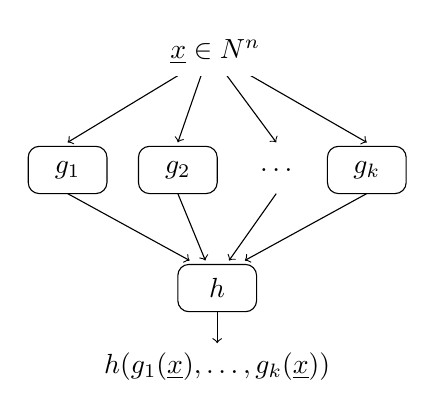
\begin{tikzpicture}
    
    \draw[->]   (0,3)--(-1.9,1.85);
    \draw[->] (-.1,3)--(-.5,1.85);
    \draw[->] (-.1,3)--(.75,1.85);
    \draw[->] (-.1,3)--(1.9,1.85);
    \draw (-2.4,1.2)[rounded corners] rectangle (-1.4,1.8)
        node[midway] {$g_1$};
    \draw (-1,1.2)[rounded corners] rectangle (0,1.8)
        node[midway]  {$g_2$};
    \node at(0.75,1.5) {$\dots$};
    \draw (1.4,1.2)[rounded corners]  rectangle (2.4,1.8) node[midway]  {$g_k$};
    
    \draw (-.53,2.7)[fill=white,white] rectangle (.48,3.3)
        node[midway,black] {$\underline{x} \in \mathbb{N}^n$};
    \draw (-.5,-.3)[rounded corners,fill=white] rectangle (.5,.3) node[midway] {$h$};

    \draw[->] (-1.9,1.2)--(-.35,.35);
    \draw[->] (-.5,1.2)-- (-.15,.35);
    \draw[->] (.75,1.2)-- (.15, .35);
    \draw[->] (1.9,1.2)-- (.35, .35);
    \draw[->] (0,-.3)--(0,-.7);
    \node at(0,-1) {$h(g_1(\underline{x}),\dots,g_k(\underline{x}))$};

\end{tikzpicture}

\end{center}

La funzione $\com$ è \textit{intuitivamente} calcolabile partendo da funzioni calcolabili: prima eseguo le singole funzioni $g_1, \dots, g_k$, poi applico la funzione $h$ sui risultati.

Calcoliamo ora la \textbf{chiusura} di $\elem$ rispetto a $\com$, ovvero l'insieme $\elem^\com$. La funzione $f(x) = x + 2$ appartiene a questo insieme perché:
$$ \com(s,s)(x) = s(s(x)) = (x + 1) + 1 = x + 2 $$

Di conseguenza tutte le funzioni lineari del tipo $f(x) = x + k$ con $k$ prefissato apparterranno all'insieme. 

Ma la funzione somma $\text{somma}(x,y) = x+y$, senza valori prefissati, non appartiene all'insieme, quindi doppiamo ampliare $\elem^\com$ con altre operazioni.

\subsubsection{Ricorsione Primitiva}

Definiamo un'operazione che permetta di \textbf{iterare} sull'operatore di composizione, la \textbf{ricorsione primitiva}, usata per definire funzioni ricorsive.

Siano:
\begin{itemize}
	\item $g: \mathbb{N}^n \rightarrow \mathbb{N}$ funzione \textbf{caso base}

	\item $h: \mathbb{N}^{n+2} \rightarrow \mathbb{N}$ funzione \textbf{passo ricorsivo}

	\item $\underline{x} \in \mathbb{N}^n$ \textbf{input}
\end{itemize}

Definiamo
$$
\rp (h,g) = f(\underline{x}, y) = \begin{cases}
	g(\underline{x}) & \text{ se } y = 0 \\
	h(f(\underline{x}, y-1), y-1, \underline{x}) & \text{ se } y > 0 \\
\end{cases}
$$

Funzione che generalizza la definizione ricorsiva di funzioni, e senza starci troppo è facilmente implementabile.

\textbf{Chiusura} di $\elem^\com$ rispetto a $\rp$ vuol dire calcolare l'insieme $\elem^{\{\com, \rp\}}$. Chiamiamo
$$ \ricprim = \elem^{\{\com, \rp\}} $$
l'insieme ottenuto dalla chiusura, cioè l'insieme delle funzioni ricorsive primitive.

In questo insieme abbiamo la somma, infatti: 
$$
\somma(x,y) = \begin{cases}
	\pro_1^2 (x,y) & \text{ se } y = 0 \\
	s (\somma(x, y-1)) & \text{ se } y > 0 \\
\end{cases}
$$
Altre funzioni in $\ricprim$:
$$ 
\prodotto (x,y) = \begin{cases}
	0^2 (x,y) & \text{ se } y = 0 \\
	\somma(x, \prodotto(x, y-1)) & \text{ se } y > 0 \\
\end{cases}
$$

$$
\predecessore \, P(x) = \begin{cases}
	0 & \text{ se } x = 0 \\
	x-1 & \text{ se } x > 0
\end{cases}
\implies 
x \dotminus y = \begin{cases}
	x & \text{ se } y = 0 \\
	P(x) \dotminus (y-1) & \text{ se $y > 0$}
\end{cases}
$$

\subsubsection{$\ricprim$ vs $\while$}

L'insieme $\ricprim$ contiene \textit{molte funzioni}, ma dobbiamo capire se ha raggiunto l'insieme $F(\while)$.

$\ricprim$ è definito come: 
\begin{itemize}
	\item $\forall f \in \elem \implies f \in \ricprim$ \hfill BASE
	
    \item Se $h, g_1, \dots, g_k \in \ricprim \implies \com(h, g_1, \dots, g_k) \in \ricprim$ \hfill PASSI
	
    \item Se $g,h \in \ricprim \implies \rp (g,h) \in \ricprim$ \hfill PASSI
	
    \item Nient'altro sta in $\ricprim$ \\
\end{itemize}

%%%%%%%%%%%%%%%%%%%%%%%%%%%%%%%%%%%%%%%%%%%%%%%%
% TODO From Here
%%%%%%%%%%%%%%%%%%%%%%%%%%%%%%%%%%%%%%%%%%%%%%%%

\begin{theor}
	$\ricprim \subseteq F(\while)$
\end{theor}
\begin{proof} \hspace{1cm} \\
	\textbf{Passo Base:} Le funzioni di $\elem$ sono ovviamente while-programmabili.
	
	\textbf{Passo Induttivo:} Per $\com$, assumiamo per ipotesi induttiva che $h,g_1, \dots, g_k \in \ricprim$ siano while-programmabili, allora esistono $H, G_1, \dots, G_K \in \wprog$ tali che $\Psi_H = h$, $\Psi_{G_1} = g_1, \dots$, $\Psi_{G_k} = g_k$.\\
	Un programma $W$ $\while$ che calcola $\com$ è
	
	\begin{center}
		\begin{minipage}{0.85\textwidth}
			\begin{tcolorbox}[colback=white,sharp corners,boxrule=.3mm]
				\begin{algorithm}[H]
					\setstretch{1.2}
					\SetArgSty{relax}
					\SetAlgoNoEnd
					\SetKwSty{texttt}
					\tcp{Inizialmente in $x_1$ ho $x$}
					$x_1 := \underline{x}$ \\
					\Begin{
						$x_0 := G_1 (x_1)$; \\
						$x_0 := [x_0, G_2 (x_1)]$; \\
						$\dots$ \\
						$x_0 := [x_0, G_k (x_1)]$ \tcp*{$x_0 := [G_1(\underline{x}), \dots, G_k (\underline{x})]$}
						$x_1 := H(x_0)$ \tcp*{$x_0 := H(G_1(\underline{x}), \dots, G_k (\underline{x}))$}
					}
					\texttt{end}
				\end{algorithm}
			\end{tcolorbox}
		\end{minipage}
	\end{center}
	
	Quindi abbiamo $\Psi_W (\underline{x}) = \com (h, g_1, \dots, g_k) (\underline{x})$.
	
	Per $\rp$, assumiamo che $h,g \in \ricprim$ siano while-programmabili, allora esistono $H,G \in \wprog$ tali che $\Psi_H = h$ e $\Psi_G = g$. Le funzioni ricorsive primitive le possiamo vedere come delle iterazioni che, partendo dal caso base $G$, mano a mano compongono con $H$ fino a quando non si raggiunge $y$ (escluso). Mostriamo un programma $\while$ che calcola
	$$ 
	\rp (h,g) = f(\underline{x}, y) = \begin{cases}
		g(\underline{x}) & \text{ se } y = 0 \\
		h(f(\underline{x}, y-1), y-1, \underline{x}) & \text{ se } y > 0
	\end{cases}
	$$
	
	\begin{center}
		\begin{minipage}{0.85\textwidth}
			\begin{tcolorbox}[colback=white,sharp corners,boxrule=.3mm]
				\begin{algorithm}[H]
					\setstretch{1.2}
					\SetArgSty{relax}
					\SetAlgoNoEnd
					\SetKwSty{texttt}
					\tcp{Inizialmente in $x_1$ ho $\langle \underline{x},y \rangle$}
					input($\underline{x},y$) \\
					\Begin{
						$t:= G(\underline{x})$; \hfill \tcp{$t$ contiene $f(\underline{x},y)$}
						$k:= 1$; \\
						\While{$k \leq y$}{
							\Begin{
								$t:= H(t, k-1, x)$; \\
								$k := k + 1$;\\
							}
							\texttt{end}
						}
					}
					\texttt{end}
				\end{algorithm}
			\end{tcolorbox}
		\end{minipage}
	\end{center}
	
	Quindi $\Psi_W (\langle x,y \rangle) = \rp (h,g) (\underline{x}, y)$.\\
\end{proof}

Abbiamo dimostrato che $\ricprim \subseteq F(\while)$ e possiamo anche dire che l'\textit{inclusione è propria}: nel linguaggio $\while$ si possono avere cicli infiniti mentre in $\ricprim$ no in quanto contiene solo funzioni totali (si dimostra per induzione strutturale) mentre $\while$ contiene anche delle funzioni parziali. Di conseguenza
$$ \ricprim \subsetneq F(\while) $$

\subsubsection{Sistema di calcolo $\for$}

Per poter \textit{raggiungere} $F(\while)$ bisognerà ampliare $\ricprim$. Visto che le funzioni in $\ricprim$ sono tutte totali, ogni ciclo in $\ricprim$ ha un inizio e una fine ben definiti: il costrutto utilizzato per dimostrare $\rp \in F(\while)$ nella dimostrazione precedente permette di definire un nuovo tipo di ciclo, il \textbf{ciclo FOR}
\begin{center}
	\begin{minipage}{.85\textwidth}
		\begin{tcolorbox}[colback=white,sharp corners,boxrule=.3mm]
			\begin{algorithm}[H]
				\setstretch{1.2}
				\SetArgSty{relax}
				\SetAlgoNoEnd
				\SetKwSty{texttt}
				input($x,y$) \\
				\Begin{
				$t:= G(x)$; \\
				\For{$k:=1$ \texttt{to} $y$}{
					$t:= H(t, k-1, x)$; \\
					}
				}
				\texttt{end}
			\end{algorithm}
		\end{tcolorbox} 
	\end{minipage}
\end{center}

Il $\for$ è un costrutto che si serve di una variabile di controllo che parte da un preciso valore e arriva a un valore limite, senza che la variabile di controllo venga toccata.

Il $\for$ language è quindi un linguaggio $\while$ dove l'istruzione di loop è un \texttt{for}. Possiamo quindi dire che $\ricprim = F(\for) \subset F(\while)$.

Dato che $\while$ sembra "vincere" su $\ricprim$ solo per i loop infiniti, restringiamo $\while$ imponendo loop finiti. Creiamo
$$ \tilde F (\while) = \{ \Psi_W: W \in \wprog \wedge \Psi_W \text{ è totale}\}$$
Ma dove si posiziona questo insieme rispetto a $\ricprim$? L'inclusione è propria? La risposta è sì, ci sono funzioni in $\tilde F (\while)$ non riscrivibili come funzioni in $\ricprim$. Un esempio è la funzione di Ackermann
$$ 
\mathcal{A} (m,n) = \begin{cases}
	n + 1 & \text{ se } m = 0 \\
	\mathcal{A}(m-1, 1) & \text{ se } m > 0 \wedge n = 0 \\
	\mathcal{A}(m-1, \mathcal{A}(m, n-1)) & \text{ se } m > 0 \wedge n > 0
\end{cases}
$$

La quale non appartiene a $\ricprim$, per causa della doppia ricorsione cresce troppo in fretta.

Questo mostra che il sistema WHILE è più potente delle funzioni in $\ricprim$, anche escludendo le funzioni parziali.

\subsection{Ampliamento di $\ricprim$}
Siamo nella "\textit{direzione giusta}" non avendo cose che non avremmo catturato in $F(\ram)$, ma questo non basta: mancano da catturare le funzioni parziali.

\begin{center}
	\scalebox{0.8}{\begin{tikzpicture}[scale=1.5]
	\draw[fill=orange!40] (2,0) ellipse (3.9 and 2.3);
	\draw[fill=cyan!40] (.9,0) ellipse  (2.6 and 1.4);
	\draw[fill=red!40] (0,0) ellipse   (1.5 and 1);
	\draw (3.4,0) ellipse (5.5 and 3);
	
	\node at (7.4,0){$F(\text{WHILE})=F(\text{RAM})$};
	\node at (2,1.65){$\elem^{\comp,\rp}=\ricprim=F(\text{FOR})$};
	\node at (-.25,.5){$\elem$};
	\node at (0,.2){\textbullet Successore};
	\node at (-.3,-.1){\textbullet Zero};
	\node at (0,-.4){\textbullet Proiezione};
	\node at (2.1,.7){$\elem^\comp$};
	\node at (2.2,-.5){$\overset{\text{\textbullet}}{f(x)=x+2}$};
	\node at (4.2,-.9){$\overset{\text{\textbullet}}{\text{somma}(x,y)=x+y}$};
	\node at (6.72,-1.3){$\overset{\text{\textbullet}}{\mathcal{A}(m,n)=\text{Ackermann}}$};
\end{tikzpicture}}
\end{center}

\subsubsection{Minimalizzazione}

Introduciamo un operatore per permettere la presenza di funzioni parziali: \textbf{minimalizzazione}. Sia $f: \mathbb{N}^{n+1} \rightarrow \mathbb{N}$ con $f(\underline{x}, y)$ e $\underline{x} \in \mathbb{N}^n$, allora: 
$$
\MIN (f) (\underline{x}) = g(\underline{x}) = \begin{cases}
	y & \text{ se } f(\underline{x}, y) = 0 \wedge (\forall y' < y, f(\underline{x}, y') \downarrow \wedge f(\underline{x}, y') \neq 0) \\
	\bot & \text{ altrimenti}
\end{cases}
$$

Un'altra definizione di $\MIN$ è 
$$ \mu_y (f(\underline{x}, y) = 0)$$

Informalmente, restituisce il più piccolo valore di $y$ che azzera $f(\underline{x},y)$, ovunque precedentemente definita su $y'$.

Alcuni esempi con $f: \mathbb{N}^2 \rightarrow \mathbb{N}$
\begin{center}
	\begin{tabular}{c|c}
		$\bm{f(x,y)}$ & $\bm{\MIN(f)(x)=g(x)}$ \\ 
		\hline
		$x+y+1$ & $\bot$\\
		$x \dotminus y$ & $x$\\
		$y \dotminus x$ & $0$\\
		$x \dotminus y^2$ & $\left\lceil\sqrt{x}\right\rceil$\\
		$\left\lfloor\frac{x}{y}\right\rfloor$ & $\bot$\\
	\end{tabular}
\end{center}

\subsection{Classe $\cp$}
Ampliamo $\ricprim$ chiudendolo con l'operazione $\MIN$
$$ \elem^{\{\com, \rp, \MIN\}} = \cp = \{\text{Funzioni Ricorsive Parziali}\}$$
Abbiamo ottenuto la classe delle \textbf{funzioni ricorsive parziali}.

\subsubsection{$\cp$ vs $\while$}

Vogliamo ora analizzare come $\cp$ si pone rispetto a $F(\while)$, sapendo che \textit{sicuramente} amplia $\ricprim$.\\

\begin{theor}
	$\cp \subseteq F(\while)$.
\end{theor}
\begin{proof}
	$\cp$ è definito per chiusura, ma si può anche definire induttivamente:
	\begin{itemize}
		\item le funzioni $\elem$ sono in $\cp$
		\item se $h, g_1, \dots, g_k \in \cp$ allora $\com (h, g_1, \dots, g_k) \in \cp$
		\item se $h,g \in \cp$ allora $\rp (h,g) \in \cp$
		\item se $f \in \cp$ allora $\MIN(f) \in \cp$
		\item nient'altro in $\cp$
	\end{itemize}
	
	Di conseguenza, per induzione strutturale su $\cp$ dimostriamo:
	\begin{itemize}
		\item \textbf{Passo base:} le funzioni elementari sono while-programmabili, come già dimostrato
		\item \textbf{Passi induttivi:}
		\begin{itemize}
			\item siano $h,g_1, \dots, g_k \in \cp$ while-programmabili per I.H., allora mostro che $\com (h, g_1, \dots, g_k)$ è while-programmabile; già fatto per $\ricprim$
			\item siano $h,g \in \cp$ while-programmabili per I.H., mostro che $\rp(h,g)$ è while-programmabile; già fatto per $\ricprim$
			\item sia $f \in \cp$ while-programmabile e sia $f$ calcolabile nel programma $\while$ per I.H., mostro che $\MIN(f)$ è while-programmabile. Devo trovare un programma $\while$ che calcoli la minimizzazione:
			\begin{center}
				\begin{minipage}{.85\textwidth}
					\begin{tcolorbox}[colback=white,sharp corners,boxrule=.3mm]
						\begin{algorithm}[H]
							\setstretch{1.2}
							\SetArgSty{relax}
							\SetAlgoNoEnd
							\SetKwSty{texttt}
							$P \equiv$ input($\underline{x}$) \\
							\Begin{
							$y:= 0$; \hfill \tcp{parte da 0}
							\While{$F(\underline{x}, y) \neq 0$}{
								$y := y + 1$; \hfill \tcp{aumenta di 1}
								}
							}
							\texttt{end}
						\end{algorithm}
					\end{tcolorbox} 
				\end{minipage}
			\end{center}
			Questo è un programma che calcola la minimizzazione: se non esiste $y$ che azzeri $f(\underline{x}, y)$ il programma va in loop (i.e., incrementa di 1 ad ogni iterazione e termina quando azzera la funzione), quindi la semantica di $P$ è $\bot$ secondo $\MIN$
		\end{itemize}
		Concludiamo quindi che $\cp \subseteq F(\while)$.
	\end{itemize}
  \end{proof}

\vspace{-0.5cm}

Viene naturale chiedersi se vale la relazione inversa.

\begin{theor}
	$F(\while) \subseteq \cp$.
\end{theor}
\begin{proof}
	Sappiamo che
	$$ F(\while) = \{\Psi_W: W \in \wprog\}$$
	Consideriamo $\Psi_W \in F(\while)$ e mostriamo che $\Psi_W \in \cp$, facendo vedere che può essere espressa come composizione, ricorsione primitiva e minimalizzazione a partire dalle funzioni in $\elem$.\\
	
	Le funzioni in $\wprog$ sono nella forma
	$$ \Psi_W = \pro_0^{21} \left( \llbracket W \rrbracket (W\text{-in}(\underline{x})) \right) $$
	Dove: 
	\begin{itemize}
		\item $\llbracket C \rrbracket (\underline{x}) = \underline{y}$ la funzione che restituisce lo stato prossimo $\underline{y} \in \mathbb{N}^{21}$ a seguito dell'esecuzione del comando $C$ a partire dallo stato corrente $\underline{x} \in \mathbb{N}^{21}$
		
		\item La funzione $W\text{-in}(n)$ restituisce lo stato iniziale della macchina $\while$ su input $n$
		
		\item $\pro_0^{21}$ preleva l'output dal registro $x_0$
	\end{itemize}
	
	Abbiamo definito $\Psi_W$ come composizione delle funzioni $\pro_0^{21}$ e $\llbracket W \rrbracket (W\text{-in}(\underline{x}))$, ma allora
	\begin{enumerate}
		\item $\pro_0^{21} \in \elem \implies \pro_0^{21} \in \cp$
		\item $\cp$ è chiuso rispetto alla composizione
	\end{enumerate}
	Di conseguenza, se dimostro che la funzione di stato prossimo $\llbracket C \rrbracket$ è ricorsiva parziale $\in \cp$ allora anche $\Psi_W \in \cp$, per la definizione induttiva di $\cp$.
	
	La funzione di stato prossimo $\llbracket \rrbracket (): \mathbb{N}^{21} \rightarrow \mathbb{N}^{21}$ restituisce elementi in $\mathbb{N}^{21}$, mentre gli elementi in $\cp$ hanno codominio $\mathbb{N}$.
	
	Per risolvere il problema si definisce la \textbf{funzione $f_C$ numero prossimo} in cui viene applicato Cantor sull'array degli stati.
	$$ \llbracket C \rrbracket \underline{x} = \underline{y} \quad \text{con }
	\ \ \underline{x},\underline{y}\in \mathbb{N}^{21}$$
	$$ f_C(x)=y \quad \text{con }
	\ \ x=[ \underline{x} ] ,\ y= [ \underline{y} ]$$
	Si noti che per passare da $\llbracket C \rrbracket (\underline{x})$ a $f_C(x)$ 
	si usano operazioni ricorsive parziali:
	$$\begin{aligned}
		f_C(x)&=y \\
		{\color{red}\pro \in \cp}\quad &
		\mathlarger{{\color{red}\downarrow}{\color{blue}\uparrow}}
		\quad\color{blue} [ \ ] \in \cp \\
		\llbracket C \rrbracket (\pro(0,x),\dots,\pro(20,x))& =(\pro(0,y),\dots,\pro(20,y))
	\end{aligned}$$
	
	Quindi si ha che $f_C$ si comporta come $\llbracket C \rrbracket (\underline{x})$ sullo stato prossimo. Basterà ora dimostrare che $f_C$ è effettivamente una funzione ricorsiva parziale:
	$$ f_C\in \cp \ \ \Leftrightarrow \ \ \llbracket C \rrbracket (\underline{x}) \in \cp $$
	Dimostriamo, tramite induzione strutturale, sul comando $\while$ $C$:
	\begin{itemize}
		\item \textbf{Passo base}: azzeramento e incremento/decremento
		\begin{itemize}
			\renewcommand{\labelitemii}{\raisebox{5.2\height}{$-$}}
			\item $\begin{aligned}
				&C\equiv \boxed{x_k:=0} \\[.6em]
				&\hspace{2em}f_C(x) = {\color{red}[}
				{\color{red}\pro}(0,x),\dots,{\color{red}0},\dots,{\color{red}\pro}
				(20,x){\color{red}]}\\
				&\hspace{10.05em}\overset{\uparrow}{\text{posizione $k$}}\\
				& \text{Viene usata una composizione di {\color{red}funzioni 
						$\in\cp$}}
				\ \Rightarrow \ f_{x_k:=0}\in\cp
			\end{aligned}$
			\renewcommand{\labelitemii}{\raisebox{5.2\height}{$-$}}
			\item $\begin{aligned}
				&C\equiv \boxed{x_k:=x_j+/\dotminus 1}\\[.6em]
				&\hspace{2em}f_C(x) = {\color{red}[}
				{\color{red}\pro}(0,x),\dots,
				{\color{red}\pro}(j,x){\color{red}+/\dotminus 1}
				,\dots,{\color{red}\pro}
				(20,x){\color{red}]}\\
				&\hspace{10.05em}\overset{\uparrow}{\text{posizione $k$}}\\
				& \text{Viene usata una composizione di {\color{red}funzioni 
						$\in\cp$}}
				\ \Rightarrow \ f_{x_k:=x_j\pm1}\in\cp
			\end{aligned}$
		\end{itemize}

		\newpage

		\item \textbf{Passi induttivi}: i comandi "complessi" $\while$ devono rientrare in $\cp$
		\begin{itemize}
			\renewcommand{\labelitemii}{\raisebox{2.1\height}{$-$}}
			\item $\begin{aligned}
				&C\equiv \boxed{
					\text{\texttt{begin} } C_ 1; \ C_2; \ \dots; \ C_m; \text{\texttt{ end}}
				}\\[.6em]
				&\hspace{2em}f_C(x) = f_{C_m}(\dots f_{C_1}(x)\dots)\\
			\end{aligned}$
			\vspace{.7em}
			
			Viene usata una composizione di $f_{C_i}$ ognuna delle quali è $\in\cp$ per ipotesi induttiva $\ \Rightarrow \ f_{C} \in \cp $
			
			\renewcommand{\labelitemii}{\raisebox{2.1\height}{$-$}}
			\item $\begin{aligned}
				&C'\equiv \boxed{\text{\texttt{while} } x_k \neq 0 \text{ \texttt{do }} C}\\[.6em]
				&\hspace{2em}f_{C'}(x) = f_C^{e(x)}(x)
				\ \ \text{ con } \ e(x)=\mu_y(\pro(k,f_C^y(x)) = 0)\\
			\end{aligned}$
			
			Sorge qui un problema: $e(x)$ non è costante; non basta quindi la composizione in quanto può essere applicata solo su un numero costante di funzioni.
			
			Si dovrà allora definire una funzione $T\in\cp$:
			$$ T(x,y)=f_C^y(x) $$
			È facile farlo usando l'operatore di ricorsione primitiva $\rp$:
			$$ T(x,y) = \begin{cases}
				x & \text{ se } y=0 \\
				f_C(T(x,y-1)) & \text{ se } y > 0
			\end{cases} $$
			Siccome:
			\begin{enumerate}
				\item $f_C \in \cp$ per ipotesi induttiva
				\item $\rp \in \cp$
			\end{enumerate}
			$$ \implies \ T(x,y)\in \cp$$
			L'ultima cosa da sistemare è $e(x)$:
			$$ \begin{aligned}
				e(x) & = \mu_y (\pro(k,f_c^y(x))=0) \\
				& =\mu_y(\pro(k,T(x,y)) = 0)
			\end{aligned} $$
			la quale è una minimalizzazione di $T(x,y) \in \cp$, quindi $e(x)\in\cp$.
			
			In conclusione:
			$$ f_{C'}(x) = f_C^{e(x)} (x) = {\color{red}T}(x,{\color{red}e}(x)) $$
			$f_{C'}$ è formato da una composizione di funzioni $\in\cp$, $ \implies f_{C'} \in \cp$. \\
		\end{itemize}
	\end{itemize}
\end{proof}
Visti i risultati ottenuti dai due teoremi precedenti, possiamo concludere che: 
$$ F(\while) = \cp $$
La classe delle funzioni ricorsive parziali, ovvero l'idea di \textit{calcolabile} in termini matematici, coincide con l'idea di \textit{calcolabile} proveniente dall'insieme di problemi per i quali vediamo una macchina che li risolva.\\

\subsection{Tesi di Church-Turing}
Il risultato principale di questo studio è aver trovato due classi di funzioni importanti: 
\begin{itemize}
	\item $\cp$ insieme delle \textbf{funzioni ricorsive parziali}
	\item $\mathcal{T}$ insieme delle \textbf{funzioni ricorsive totali}
\end{itemize}

Il primo insieme contiene anche tutte le funzioni del secondo, quindi
$$ \mathcal{T} \subset \cp $$
Inoltre abbiamo visto (ad esempio tramite la funzione di Ackermann) che
$$ \ricprim \subset \mathcal{T} $$
L'insieme $\cp$ cattura tutti i sistemi di calcolo esistenti: $\while$, $\ram$, Macchine di Turing, Lambda-calcolo di Church, \dots\\
Tutti i modelli di calcolo proposti alla fine individuano sempre la classe delle funzioni ricorsive parziali. Visti questi risultati, Church e Turing decidono di enunciare un risultato molto importante.

\paragraph{Tesi di Church-Turing:} La classe delle funzioni intuitivamente calcolabili coincide con la classe $\cp$ delle funzioni ricorsive parziali.

Questa è una tesi e non un teorema, si tratta di una \textit{congettura}, un'opinione, in quanto non è possibile caratterizzare i modelli di calcolo ragionevoli che sono stati e saranno proposti in maniera completa. Possiamo solo decidere se aderire o meno a questa tesi.

Per noi un problema è \textit{calcolabile} quando esiste un modello di calcolo che riesce a risolverlo ragionevolmente. Se volessimo aderire alla tesi di Church-Turing, potremmo dire, in maniera più formale, che:
\begin{itemize}
	\item \textit{problema ricorsivo parziale} è sinonimo di calcolabile
	\item \textit{problema ricorsivo totale} è sinonimo di calcolabile da un programma che si arresta su ogni input
\end{itemize}

\section{Assiomatizzazione dei Sistemi di Calcolo}

Per ora ci si è concentrati sull'analisi della \textit{potenza computazionale} dei sistemi di programmazione visti, affermando che ognuno di questi ha come potenza computazionale $\cp$ grazie alla tesi di Church-Turing.

Vorremmo sapere altro sui sistemi di programmazione, vogliamo individuare alcune proprietà "buone" di un sistema di calcolo, dette \textbf{assiomi}. Tutti i sistemi di programmazione che rispettano questi assiomi si diranno sistemi di programmazione accettabili. In questo modo si potranno dimostrare proprietà non sul singolo sistema ma su tutti i sistemi accettabili utilizzando appunto solo questi assiomi.

Per indicare un sistema di programmazione si usa
$$ \sisprog_{i \in \N}$$
ovvero l'insieme delle semantiche (funzioni calcolabili) dal sistema. Il pedice indica i programmi codificati $i \in \N$ di quel sistema.

\subsection{Assiomi di Rogers}

Gli assiomi di Rogers vogliono essere quelle "buone" proprietà ricercate in un sistema di programmazione; in particolare si afferma che: un sistema di programmazione $\sisprog$ si dice \textbf{accettabile} (o \textbf{SPA}) se: \\
\begin{enumerate}
	\item Aderisce alla tesi di Church-Turing
	\item Ammette interprete universale
	\item Rispetta il teorema $S_n^m$
\end{enumerate}
Si vedranno ora gli assiomi nel dettaglio.

\subsubsection{Potenza computazionale}
Dato il sistema $\sisprog$ vogliamo che
$$ \sisprog = \cp $$
ovvero, rispetta la tesi di Church-Turing. Come già dimostrato, il sistema $\ram$ rispetta il primo assioma
$$ F(\ram) = \cp $$
Non si vogliono considerare né sistemi troppo poco potenti (sotto $\cp$), né troppo potenti (oltre $\cp$).

\subsubsection{Interprete universale}
$\sisprog$ rispetta il secondo assioma se esiste un interprete universale, ovvero un programma $\mu \in \N$ tale che
$$ \forall x,n \in \N \quad \varphi_\mu (\langle x,n \rangle) = \varphi_n (x) $$
ovvero, un programma scritto in un certo linguaggio che riesce ad interpretare ogni altro programma $n$ scritto nello stesso linguaggio su qualsiasi input $x$.

La presenza di un interprete universale permette un'algebra sui programmi, quindi la trasformazione di quest'ultimi.

\subsubsection{Teorema $S_n^m$}
$\sisprog$ rispetta il terzo assioma se rispetta il teorema $S_n^m$. Si vedrà prima un teorema più specifico $S_1^1$. \\

\begin{theor}[$S_1^1$]
	Dato $\sisprog$ $\ram$ esiste una funzione $S_1^1 \in \T$ tale che
	$$ \forall n,x,y \in \N \quad \varphi_n(\langle x,y \rangle) = \varphi_{S_1^1 (n,y)} (x) $$
In altre parole, è possibile costruire automaticamente programmi specifici da programmi più generali, ottenuti fissando alcuni input.
\end{theor}

\begin{proof}
	In generale, il programma $S_1^1$ implementa la funzione
	$$ S_1^1 (n,y) = \bar{n} \tc \varphi_{\bar{n}}(x) = \varphi_n (x,y) $$
	dove:
	\begin{itemize}
		\item $n$ è la codifica del programma $P$ a due variabili di input $x,y$
		\item $\bar{n}$ è la codifica del programma $\bar{P}$ a una variabile, la cui semantica è identica a quella di $P$ a cui fisso a $y$ il secondo input
	\end{itemize}

	Analizzando il sistema $\ram$ si prenda un programma $P$ a due variabili
	$$ P \in \prog \mid \varphi_P (\langle x,y \rangle) = x + y $$

	\vspace{-2.2em}
	\begin{minipage}{.4\textwidth}
		\begin{align}
			P \equiv\ & \texttt{// input $\langle x,y \rangle$ in $R_1$}   \notag\\
			& R_2 \leftarrow \sin(R_1)                     \notag\\
			& R_3 \leftarrow \des(R_1)                      \notag\\
			& R_0 \leftarrow R_2+R_3                       \notag
		\end{align}
	\end{minipage}
	\begin{minipage}{.4\textwidth}
		$$ \varphi_P(\langle x,y \rangle) = x + y $$
	\end{minipage}

	Si vuole produrre un programma $\bar{P}$ con un solo input $x$ che restituisca $x + 3$, partendo da $P$. Si fissa quindi la seconda variabile di $P$ a 3. La funzione $S_1^1$ dovrà restituire $\bar{P}$

	\begin{minipage}{.46\textwidth}
		\begin{center}
			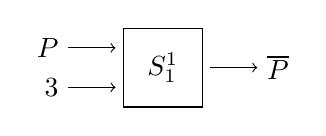
\begin{tikzpicture}
	
	\draw[->] (2.3,1.75) node[left]{$P$} -- (2.9,1.75);
	\draw[->] (2.3,1.25) node[left]{$3$} -- (2.9,1.25);
	\draw (3,2) rectangle (4,1);
	\node at (3.5,1.5) {$S_1^1$};
	\draw[->] (4.1,1.5) -- (4.7,1.5)
	node [right] {$\overline{P}$};
	
\end{tikzpicture}
		\end{center}
	\end{minipage}
	\begin{minipage}{.46\textwidth}
		\begin{tabular}{r l l}
			$\bar{P}\equiv$ & $\texttt{// input $x$ in $R_1$}$ & \\
			& $R_0 \leftarrow R_0 + 1$ &
			\multirow{3}{*}{\hspace{-2em}
				$\begin{rcases}
					\phantom{}\\
					\phantom{}\\
				\end{rcases}$ fissa $y$ a 3
			}\\

			& $R_0 \leftarrow R_0+1$ & \\
			& $R_0 \leftarrow R_0+1$ & \\

			& $R_1 \leftarrow \langle R_1,R_0\rangle$ &
			\hspace{-2em}
			$\begin{rcases}
				\phantom{}
			\end{rcases}$ input di $P$\\

			& $R_0 \leftarrow 0$  &
			\hspace{-2em}
			$\begin{rcases}
				\phantom{}
			\end{rcases}$ pulisci $R_0$\\

			& $P$ &
			\hspace{-2em}
			$\begin{rcases}
				\phantom{}
			\end{rcases}$ richiama $P$
		\end{tabular}
	\end{minipage}

	Si consideri il programma $\bar{P}$ nel caso generale, fissando la seconda variabile a un valore $y$:
	\begin{center}
		\begin{tabular}{r l l c c}
			$\bar{P}\equiv$ & $\texttt{// input $x$ in $R_1$}$
			&&codifica & \\
			& $R_0 \leftarrow R_0+1$ &
			\multirow{3}{*}{\hspace{-2em}
				$\begin{rcases}
					\phantom{}\\
					\phantom{}\\
					\phantom{}\\
				\end{rcases} y$ volte
			} & $\longmapsto$ & 0 \\
			& $\hspace{2.6em}\vdots$ & & $\vdots$  & \\
			& $R_0 \leftarrow R_0+1$ & & $\longmapsto$ & 0  \\
			& $R_1 \leftarrow \langle R_1,R_0 \rangle$ &
			\hspace{-2em}
			$\begin{rcases}
				\phantom{}
			\end{rcases}$ input di $P$ & $\longmapsto$ & s\\
			& $R_0 \leftarrow 0$  &
			\hspace{-2em}
			$\begin{rcases}
				\phantom{}
			\end{rcases}$ pulisci $R_0$ & $\longmapsto$ & t\\
			& $R_0 \leftarrow R_2+R_3$ &
			\hspace{-2em}
			$\begin{rcases}
				\phantom{}
			\end{rcases}$ richiama $P$ & $\longmapsto$ & n
		\end{tabular}
	\end{center}

	La codifica del programma $\bar{P}$ è
	$$ cod(\bar{P}) = \bar{n} = \langle \underbrace{0,\dots,0}_{y\text{ volte}},s,t,n \rangle = S^1_1 $$
	con $s$ codifica dell'istruzione che calcola la funzione coppia di Cantor e $t$ codifica dell'istruzione di azzeramento.

	Si può quindi notare che $S_1^1$ è
	\begin{enumerate}
		\item Una funzione totale
		\item Programmabile
	\end{enumerate}
	Di conseguenza
	$$ S_1^1 \in \T $$
\end{proof}

In sintesi, per $\ram$, esiste una funzione $S_1^1$ ricorsiva totale che accetta come argomenti
\begin{itemize}
	\item il codice $n$ di un programma con 2 input
	\item un valore $y$ a cui fissare il secondo input
\end{itemize}
e produce il codice $\bar{n} = S^1_1 (n,y)$ di un programma che si comporta come $n$ nel caso in cui il secondo input è fissato a $y$. \lcomment{Il Teorema $S^1_1$ da solo garantisce una ``algebra sui programi'' }

Questo teorema ha anche una forma generale $S_n^m$ che riguarda i programmi a $m+n$ input in cui si prefissano $n$ input e si lasciano variare i primi $m$.\\

\begin{theor}[$S_n^m$]
	Dato $\sisprog$ $\ram$, esiste una funzione $S_n^m \in \T$ tale che
	$$ \forall  \in \N, \underline{x} \in \N^m, \underline{y} \in \N^n \quad \varphi_k (\langle \underline{x}, \underline{y} \rangle) = \varphi_{S_n^m (k, \underline{y})} (\langle \underline{x} \rangle) $$
	Ovvero, per ogni programma $k \in \N$ e ogni input $\underline{x} \in \N^m, \underline{y} \in \N^n$ vale la proprietà specificata. Anche la dimostrazione è una semplice generalizzazione di quella di $S_1^1$.\\
\end{theor}

Le tre caratteristiche identificate formano gli \textbf{assiomi di Rogers} (1953). Questi caratterizzano i sistemi di programmazione su cui ci concentreremo, chiamati \textit{Sistemi di Programmazione Accettabili}. Questi assiomi non sono restrittivi: di fatto, tutti i modelli di calcolo ragionevoli sono SPA.

\subsection{Compilatori tra SPA}

Dati gli SPA $\{\varphi_i\}$ e $\{\Psi_i\}$, un compilatore dal primo al secondo è una funzione $t : \N \rightarrow \N$ che soddisfa le proprietà di
\begin{enumerate}
	\item \textbf{programmabilità}: esiste un programma che implementa $t$
	\item \textbf{completezza}: $t$ compila ogni $i \in \N$
	\item \textbf{correttezza}: $\forall i \in \N$ vale $\varphi_i = \Psi_{t(i)}$
\end{enumerate}

Visto quanto fatto fin'ora, si può dire che i primi due punti possono essere scritti come $t \in \T$.\\

\begin{theor}
	Dati due SPA, esiste sempre un compilatore tra essi.
\end{theor}
\begin{proof}
	Consideriamo $\{\varphi_i\}$ e $\{\Psi_i\}$ due SPA; valgono i tre assiomi di Rogers:
	\begin{enumerate}
		\item $\{\varphi_i\} = \cp$
		\item $\exists u: \varphi_u (\langle x,n \rangle) = \varphi_n (x)$
		\item $\exists S_1^1 \in \T: \varphi_n (\langle x,y \rangle ) = \varphi_{S^1_1 (n,y)} (x)$
	\end{enumerate}

	Voglio trovare un compilatore $t \in \T$ che sia corretto. Ma allora
	$$ \varphi_i (x) \stackrel{(2)}{=} \varphi_u (\langle x,i \rangle ) \stackrel{(1)}{=} \Psi_e (\langle x,i \rangle) \stackrel{(3)}{=} \Psi_{S_1^1(e,i)} (x) $$

	Ovvero, il compilatore cercato è la funzione $t(i) = S^1_1 (e,i)$ per ogni $i \in \N$. Infatti:
	\begin{itemize}
		\item $t \in \T$ in quanto $S_1^1 \in \T$
		\item $t$ corretto perché $\varphi_i = \Psi_{t(i)}$
	\end{itemize}
\end{proof}

Da notare che questo teorema è molto generale, specifica solamente che il compilatore esiste, non determina quale sia. \\

\begin{coroll}
	Dati gli SPA $A,B,C \ \ \exists$sempre un compilare da $A$ a $B$ scritto nel linguaggio $C$.
\end{coroll}
\begin{proof}
	Per il teorema precedente esiste un compilatore $t \in \T$ da $A$ a $B$. $C$ è un SPA, quindi contiene programmi per tutte le funzioni ricorsive parziali, dunque ne contiene uno anche per $t$, che è una funzione ricorsiva totale. \\
\end{proof}

Nella pratica, vuol dire che per qualunque coppia di linguaggi, sarà sempre possibile scrivere un compilatore tra essi in un altro linguaggio arbitrario. Un risultato più forte del teorema precedente è invece dato dal \textbf{teorema di Rogers}.\\

\begin{theor}[Teorema di isomorfismo tra SPA]
	Dati due SPA $\{\varphi_i\}$ e $\{\Psi_i\}$, esiste $t: \N \rightarrow \N$ tale che:
	\begin{enumerate}
		\item $t \in \T$ \lcomment{Teorema Precedente}
		\item $\forall i \in \N$, $\varphi_i = \Psi_{t(i)}$ \lcomment{Teorema Precedente}
		\item $t$ è invertibile, quindi $t^{-1}$ può essere visto come un decompilatore
	\end{enumerate}
\end{theor}

I primi due punti sono uguali al teorema precedente e dicono che il compilatore $t$ è programmabile e completo (punto 1) e corretto (punto 2).

\subsection{Teorema di Ricorsione}

Il teorema di ricorsione è un risultato utile a rispondere ad alcuni quesiti sugli SPA. \\

\begin{theor}
	Dato un SPA $\varphi_i$, per ogni $t: \N \rightarrow \N$ ricorsiva totale vale
	$$ \exists n \in \N \mid \varphi_n = \varphi_{t(n)} $$
\end{theor}

Per dare una chiave di lettura a questo teorema:
\begin{itemize}
	\item consideriamo $t$ come un programma che prende in input un programma $n$ è lo trasforma in $t(n)$
	\item il teorema dice che, qualsiasi sia la natura di $t$, esisterà sempre almeno un programma il cui significato non sarà stravolto da $t$
\end{itemize}

\begin{proof}
	Considerando un SPA $\{\varphi_i\}$, valgono i tre assiomi di Rogers. Per semplicità, scriveremo $\varphi_n (x,y)$ al posto di $\varphi_n (\langle x,y \rangle)$. Dobbiamo esibire, data una funzione $t$, uno specifico valore di $n$.

	Partiamo mostrando che:
	$$ \varphi_{\varphi_i (i)} (x) \stackrel{(2)}{=} \varphi_{\varphi_u (i,i)} (x) \stackrel{(2)}{=} \varphi_u (x, \varphi_u (i,i)) \rightsquigarrow f(x,i) \in \cp $$

	Infatti, la funzione $f(x,i)$ è composizione di funzioni ricorsive parziali, quindi anch'essa lo è.

	Continuiamo affermando che
	$$ f(x,i) \stackrel{(1)}{=} \varphi_e (x,i) \stackrel{(3)}{=} \varphi_{S_1^1 (e,i)} (x) $$

	Consideriamo ora la funzione $t\left(S_1^1 (e,i)\right)$: essa è ricorsiva totale in $i$ perché composizione di $t$ e di $S_1^1$ ricorsive totali, quindi
	$$ \exists m \in \N \mid \varphi_m (i) = t\left(S_1^1 (e,i)\right) $$
	Abbiamo quindi mostrato che
	\begin{align*}
		(A) \quad \quad & \varphi_{\varphi_i (i)} (x) = \varphi_{S_1^1 (e,i)} (x) \\
		(B) \quad \quad & \varphi_m (i) = t\left(S_1^1 (e,i) \right)
	\end{align*}

	Fissiamo $n = S_1^1 (e,m)$ e mostriamo che vale $\varphi_n = \varphi_{t(n)}$, ovvero il teorema di ricorsione
	$$ \varphi_n (x) \stackrel{\text{def}}{=} \varphi_{S_1^1 (e,m)} (x) \stackrel{(A)}{=} \varphi_{\varphi_m (m)} (x) $$
	$$ \varphi_{t(n)} (x) \stackrel{\text{def}}{=} \varphi_{t\left(S_1^1 (e,m)\right)} (x) \stackrel{(B)}{=} \varphi_{\varphi_m (m)} (x)$$

	Ho ottenuto lo stesso risultato, quindi il teorema è verificato.\\
\end{proof}

\subsection{Due quesiti sugli SPA}

Ci poniamo due quesiti riguardo agli SPA:
\begin{enumerate}
	\item \textbf{Programmi auto-replicanti}: dato un SPA, esiste all'interno di esso un programma che stampa se stesso (il proprio listato)? Ovviamente senza aprire il file che contiene il listato.

	Questi programmi sono detti \textbf{Quine}, in onore del filosofo e logico \href{https://it.wikipedia.org/wiki/Willard_Van_Orman_Quine}{\texttt{Willard Quine}} che li descrisse per la prima volta. La risposta è positiva per molti linguaggi; ad esempio, in Python, il programma
	\begin{minted}{python}
a='a=%r;print(a%%a)';print(a%a)
	\end{minted}
	stampa esattamente il proprio listato.

	Per rispondere rigorosamente ambientiamo la domanda nel sistema di programmazione $\ram$, che diventa:
	$$ \exists j \in \N \mid \varphi_j (x) = j \text{ per ogni input } x \in \N \text{?}$$

	\item \textbf{Compilatori completamente errati}: dati due SPA $\{\varphi_i\}$ e $\{\Psi_j\}$, esiste un compilatore completamente errato?

	Un compilatore dal primo al secondo SPA è una funzione $t: \N \rightarrow \N$ tale che
	\begin{itemize}
		\item $t \in \T$ programmabile e totale
		\item $\forall i \in \N$, $\varphi_i = \Psi_{t(i)}$
	\end{itemize}

	Invece, un \textbf{compilatore completamente errato} è una funzione $t: \N \rightarrow \N$ tale che
	\begin{itemize}
		\item $t \in \T$ programmabile e totale
		\item $\forall i \in \N$, $\varphi_i \neq \Psi_{t(i)}$
	\end{itemize}
\end{enumerate}

\subsubsection{Prima domanda: Quine}
Consideriamo il programma $\ram$

\begin{center}
\[
\begin{array}{r|l|}
    \cline{2-2}
    P \equiv & R_0 \leftarrow R_0 + 1 \\
            & R_0 \leftarrow R_0 + 1 \\
            & \dots \\
            & R_0 \leftarrow R_0 + 1 \\
    \cline{2-2}
\end{array}
\left.
\begin{array}{c}
~ \\
~ \\
~ \\
~
\end{array}
\right\} \text{ j times}
\]
\end{center}

il quale ripete l'istruzione di incremento di $R_0$ un numero $j$ di volte. La semantica di questo programma è esattamente $j$: infatti dopo la sua esecuzione avremo $j$ nel registro di output $R_0$.

Calcoliamo la codifica di $P$ come
$$ cod(P) = \underbracket{\langle 0, \dots, 0 \rangle}_{j\text{-volte}} = Z (j) \in \T $$
Questa funzione è ricorsiva totale in quanto programmabile e totale, visto che sfrutta solo la funzione di Cantor. Vale quindi:
$$ \varphi_{Z(j)} (x) = j $$
Per il teorema di ricorsione
$$ \exists j \in \N \mid \varphi_j (x) = \varphi_{Z (j)} (x) = j $$
Quindi effettivamente esiste un programma $j$ la cui semantica è proprio quella di stampare se stesso.

La risposta alla prima domanda è quindi \si! per $\ram$, ma lo è in generale per tutti i SPA che ammettono una codifica per i propri programmi.

\subsubsection{Seconda domanda: compilatori completamente errati}

Supponendo di avere una funzione $t \in \T$ che "\textit{maltratta}" i programmi. La semantica del programma "\textit{maltrattato}" $t(i)$:
$$ (\ast) \quad \quad \Psi_{t(i)} (x) \stackrel{(2)}{=} \Psi_u (x, t(i)) \stackrel{(1)}{=} \varphi_e (x, t(i)) \stackrel{(3)}{=} \varphi_{S_1^1 (e,t(i))} (x) $$

Chiamiamo $g(i)$ la funzione $S_1^1 (e, t(i))$ che dipende solo da $i$, essendo $e$ un programma fissato. Notiamo come questa funzione sia composizione di funzioni ricorsive totali, ovvero $t(i)$ per ipotesi e $S^1_1$ per definizione, quindi anch'essa è ricorsiva totale.

Per il teorema di ricorsione
$$ (\ast \ast) \quad \quad \exists i \in \N \mid \varphi_i = \varphi_{g(i)} $$

Unendo $(\ast)$ e $(\ast \ast)$ otteniamo
$$ \exists i \in \N \mid \Psi_{t(i)} \stackrel{(\ast)}{=} \varphi_{g(i)} \stackrel{(\ast \ast)}{=} \varphi_i \quad \forall t \in \T $$

Di conseguenza, la risposta alla seconda domanda è \no!.

\subsection{Equazioni su SPA}
\subsubsection{Strategia}

La portata del teorema di ricorsione è molto ampia: permette di risolvere \textbf{equazioni su SPA} in cui si chiede l'esistenza di certi programmi in SPA.

Per esempio, dato un SPA $\{\varphi_i\}$ ci chiediamo se
$$ \exists n \in \N \mid \varphi_n (x) = \varphi_x \left(n + \varphi_{\varphi_n (0)} (x) \right) $$
La strategia da seguire per risolvere questo tipo di richieste è analoga a quella seguita per la dimostrazione del teorema di ricorsione, riassumibile in:
\begin{enumerate}
	\item Trasformare il membro di destra dell'equazione in una funzione $f(x,n)$
	\item Mostrare che $f(x,n)$ è ricorsiva parziale e quindi che $f(x,n) = \varphi_e (x,n)$
	\item L'equazione iniziale diventa $\varphi_n (x) = \varphi_e (x, n) = \varphi_{S^1_1 (e,n)} (x)$
	\item So che $S^1_1 (e,n)$ è una funzione ricorsiva totale che dipende da $n$
	\item La domanda iniziale è diventata $\exists n \in \N \mid \varphi_n (x) = \varphi_{S_1^1 (e,n)} (x)$?
	\item La risposta è \si, per il teorema di ricorsione
\end{enumerate}

Riprendendo l'esempio e cominciando con trasformare la parte di destra:
\begin{align*}
	\varphi_n (x) & \stackrel{(2)}{=} \varphi_x \left(n + \varphi_{\varphi_u (0,n)} (x)\right) \\
	& \stackrel{(2)}{=} \varphi_x \left(n + \varphi_u \left(x, \varphi_u (0,n)\right)\right) \\
	& \stackrel{(2)}{=} \varphi_u \left(n + \varphi_u \left(x, \varphi_u (0,n)\right), x\right) \\
	& = f(x,n) \in \cp
\end{align*}

\vspace{-1em}

L'ultimo passaggio è vero perché $\varphi_u \left(n + \varphi_u \left(x, \varphi_u (0,n)\right), x\right)$ compone solamente funzioni ricorsive parziali quali somma e interprete universale. Di conseguenza, esiste un programma $e$ che calcola la funzione $f(x,n)$.

Continuando, l'equazione si può riscrivere come
\begin{align*}
	\varphi_n (x) & = f(x,n) \\
	& \stackrel{(1)}{=} \varphi_e (x,n) \\
	& \stackrel{(3)}{=} \varphi_{S_1^1 (e,n)} (x)
\end{align*}

con $S_1^1 (e,n) \in \T$ per l'assioma 3.\\

Per il teorema di ricorsione possiamo concludere che
$$ \exists n \in \N \mid \varphi_n (x) = \varphi_{S^1_1 (e,n)} (x) = \varphi_x \left(n + \varphi_{\varphi_u (0,n)} (x)\right) $$

\subsubsection{Esercizi}

In tutti gli esercizi viene dato un SPA $\{\varphi_i\}$

$$ \exists n \in \N \mid \varphi_n (x) = \varphi_x (n) + \varphi_{\varphi_x (n)} (n)? $$
\begin{align*}
	\varphi_n (x) & \stackrel{(2)}{=} \varphi_u (n,x) + \varphi_{\varphi_u (n,x)} (n) \\
	& \stackrel{(2)}{=} \varphi_u (n,x) + \varphi_u (n, \varphi_u (n,x)) \\
	& = f(x,n) \\
	& \stackrel{(1)}{=} \varphi_e (x,n) \stackrel{(3)}{=} \varphi_{S^1_1 (e,n)} (x) \\
	& \fin
\end{align*}

$$ \exists n \in \N \mid \varphi_n (x) = n^x + \left(\varphi_x (x)\right)^2 ? $$
\begin{align*}
	\varphi_n (x) & \stackrel{(2)}{=} n^x + \left(\varphi_u (x,x)\right)^2 \\
	& = f(x,n) \\
	& \stackrel{(1)}{=} \varphi_e (x,n) \stackrel{(3)}{=} \varphi_{S^1_1 (e,n)} (x) \\
	& \fin
\end{align*}

$$ \exists n \in \N \mid \varphi_n (x) = \varphi_x \left(\langle n, \varphi_x (1) \rangle \right) ?$$
\begin{align*}
	\varphi_n (x) & \stackrel{(2)}{=} \varphi_u \left(\langle n, \varphi_u (1, x) \rangle, x\right) \\
	& = f(x,n) \\
	& \stackrel{(1)}{=} \varphi_e (x,n) \stackrel{(3)}{=} \varphi_{S_1^1 (e,n)} (x) \\
	& \fin
\end{align*}
$$ \exists n \in \N \mid \varphi_n (x) = \varphi_{\varphi_x (\sin (n))} (\des (n)) ? $$
\begin{align*}
	\varphi_n (x) & \stackrel{(2)}{=} \varphi_{\varphi_u (\sin (n), x)} (\des (n)) \\
	& \stackrel{(2)}{=} \varphi_u (\des (n), \varphi_u (\sin (n), x)) \\
	& = f(x,n) \\
	& \stackrel{(1)}{=} \varphi_e (x,n) \stackrel{(3)}{=} \varphi_{S_1^1 (e,n)} (x) \\
	& \fin
\end{align*}
$$ \exists n \in \N \mid \varphi_n (x) = n^x + \left(\varphi_x (x)\right)^2 ?$$
\begin{align*}
	\varphi_n (x) & \stackrel{(2)}{=} n^x + \left(\varphi_u (x,x)\right)^2 \\
	& = f(x,n) \\
	& \stackrel{(1)}{=} \varphi_e (x,n) \stackrel{(3)}{=} \varphi_{S_1^1 (e,n)} (x) \\
	& \fin \\
\end{align*}
$$ \exists n \in \N \mid \varphi_n (x) = \varphi_x (n + 2) + \left(\varphi_{\varphi_x (n)} (n+3)\right)^2 ? $$
\begin{align*}
	\varphi_n (x) & \stackrel{(2)}{=} \varphi_u (n + 2, x) + \left(\varphi_{\varphi_u (n, x)} (n + 3)\right)^2 \\
	& \stackrel{(2)}{=} \varphi_u (n+2, x) + \left(\varphi_u \left(n + 3, \varphi_u (n,x)\right)\right)^2  \\
	& = f(x,n) \\
	& \stackrel{(1)}{=} \varphi_e (x,n) \stackrel{(3)}{=} \varphi_{S_1^1 (e,n)} (x) \\
	& \fin
\end{align*}


\section{Problemi di Decisione}

Un \textbf{problema di decisione} è una domanda a cui rispondere \si\ o \no. Sono costituiti da tre elementi principali:
\begin{itemize}
	\item \textbf{Nome}: del problema
	\item \textbf{Istanza}: dominio degli oggetti che verranno considerati
	\item \textbf{Domanda}: proprietà che gli oggetti del dominio possono soddisfare o meno. Dato un oggetto del dominio, la risposta sarà \si\ se soddisfa la proprietà, \no\ altrimenti. In altre parole, è la specifica del problema di decisione
\end{itemize}

Una definizione più formale:
\begin{itemize}
	\item \textbf{Nome} $\Pi$
	\item \textbf{Istanza} $x \in D$ input
	\item \textbf{Domanda} $p(x)$ proprietà che $x \in D$ può soddisfare o meno
\end{itemize}

Non bisogna esibire una struttura come risultato (cosa che puo' accadere nei problemi di ricerca od ottimizzazione), ma solo una risposta \si/\no.

\vspace{-1em}

\paragraph{Esempio:} Un esempio di problema di decisione è quello di stabilire se un grafo ammette un circuito hamiltoniano:
\begin{itemize}
	\item Nome: Circuito hamiltoniano
	\item Istanza: grafo $G = (V,E)$
	\item Domanda: $\exists \gamma$ circuito hamiltoniano nel grafo $G$?
\end{itemize} \lcomment{altri esempi nelle slide}

\vspace{-0.5em}

\subsection{Decidibilità}

Sia $\Pi$ problema di decisione con istanza $x \in D$ e domanda $p(x)$. $\Pi$ è \textbf{decidibile} se e solo se esiste un programma $P_\Pi$ tale che
\begin{center}
		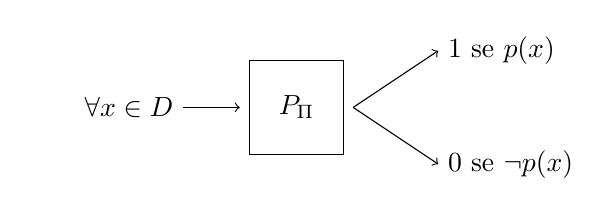
\begin{tikzpicture}[scale=1.2]
	\draw[->] (2.3,1.5) node[left]{$\forall x \in D$} -- (2.9,1.5);
	\node[left] at (2.3,1.5) {$\phantom{cod(P)=n}$};
	\draw (3,2) rectangle (4,1);
	\node at (3.5,1.5) {$P_\Pi$};
	\draw[->] (4.1,1.5) -- (5,2.1) node [right] {$1$ se $p(x)$};
	\draw[->] (4.1,1.5) -- (5,0.9) node [right] {$0$ se $\neg p(x)$};
\end{tikzpicture}
\end{center}

Allo stesso modo, possiamo associare a $\Pi$ la sua \textbf{funzione soluzione}:
$$ \Phi_\Pi : D \rightarrow \{0,1\} \tc \Phi_\Pi (x) = \begin{cases}
	1 & \text{ se } p(x) \\
	0 & \text{ se } \neg p(x)
\end{cases}$$

Questa funzione deve essere programmabile e deve terminare sempre; ma allora $\Phi_\Pi \in \T$.

I due approcci per \textbf{definire la decidibilità} sono equivalenti:
\begin{itemize}
	\item il programma $P_\Pi$ calcola $\Phi_\Pi$, quindi $\Phi_\Pi \in \T$
	\item se $\Phi_\Pi \in \T$, allora esiste un programma che la calcola e che ha il comportamento di $P_\Pi$
\end{itemize}

Quindi, definire la decidibilità partendo da un programma o da una funzione ricorsiva totale è indifferente: una definizione implica l'altra.

Si può sfruttare questo fatto per sviluppare due \textbf{tecniche di risoluzione} del problema di decidibilità:
\begin{itemize}
	\item Esibire un \textbf{algoritmo di soluzione} $P_\Pi$ (anche inefficiente, basta che esista)
	\item Mostrare che $\Phi_\Pi$ è \textbf{ricorsiva totale}
\end{itemize}

\paragraph{Esempio:} Sull'esempio precedente, dovendo visitare ogni nodo una e una sola volta, il circuito genera una permutazione dei vertici in $V$. L'algoritmo di soluzione deve:
\begin{enumerate}
	\item generare l'insieme $P$ di tutte le permutazioni di $V$
	\item data la permutazione $p_i \in P$, se è un c.h. rispondo \si
	\item se nessuna permutazione $p_i \in P$ è un c.h. rispondo \no
\end{enumerate} \lcomment{Guarda slide per robe in piu'}

\vspace{-0.25em}

\subsection{Problemi indecidibili}

Esistono dei \textbf{problemi indecidibili}? \si: se esistono programmi che non so come scrivere, allora esistono problemi per i quali non posso scrivere dei programmi che li risolvano.

\subsubsection{Problema dell'arresto ristretto}

Il \textbf{problema dell'arresto ristretto} per un programma $P$ è un esempio di problema indecidibile. Fissato un programma $P$, il problema è il seguente:
\begin{itemize}
	\item Nome: $\arp$
	\item Istanza: $x \in \N$
	\item Domanda: $\varphi_P (x) \downarrow$?
\end{itemize}

In altre parole, ci chiediamo se $P$ termina su input $x$. La risposta dipende da $P$, che può essere decidibile o meno. Per alcuni programmi si può trovare risposta ed è quindi decidibile, tuttavia esistono dei programmi dove $\arp$ è indecidibile.

Consideriamo ora il programma $\hat{P}$:
\begin{align}
	\hat{P} \equiv\ & \text{input($x$)}       \notag\\
	& Z := U(x,x)                             \notag\\
	& \text{output($Z$)}                      \notag
\end{align}

Dove $U$ è l'interprete universale tale che
$$ \varphi_U (x,n) = \varphi_n (x) $$

E definiamo di conseguenza il problema $\arph$:
$$ \varphi_{\hat{P}}(x) = \varphi_{U}(x,x) = \varphi_{x}(x) $$
\begin{itemize}
	\item Nome $\arph$
	\item Istanza $ x \in \N$
	\item Domanda: $\varphi_{\hat{P}}(x) = \varphi_x(x) \downarrow ?$
\end{itemize}

Abbiamo, quindi, un programma $x$ che lavora su un altro programma (\textit{se stesso} in questo caso). Nulla di strano: compilatori, debugger, interpreti sono programmi che lavorano su programmi.

La domanda è se $\varphi_x$ su input $x$ termina. Il programma $P$ non è fissato e dipende dall'input, essendo $x$ sia input che programma.\\

\begin{theor}[Indecidibilità di $\arph$]
	$\arph$ è indecidibile.
\end{theor}
\begin{proof}
	Per assurdo, assumiamo $\arph$ decidibile. Dunque esiste
	$$
	\Phi_{\arph} (x) = \begin{cases}
		1 & \text{ se } \varphi_{\hat{P}} (x) = \varphi_x (x) \downarrow \\
		0 & \text{ se } \varphi_{\hat{P}} (x) = \varphi_x (x) \uparrow \\
	\end{cases}
	\in \T
	$$
	calcolabile da un programma che termina sempre. Visto che $\Phi_{\arph} \in \T$ anche la funzione
	$$
	f(x) = \begin{cases}
		0 & \text{ se } \Phi_{\arph} (x) = 0 \equiv \varphi_x (x) \uparrow \\
		\varphi_x (x) + 1 & \text{ se } \Phi_{\arph} (x) = 1 \equiv \varphi_x (x) \downarrow
	\end{cases}
	$$
	è ricorsiva totale, si può avere un programma che calcola esattamente la funzione $f(x)$.

	Sia $\alpha \in \N$ la codifica del programma $A$, tale che $\varphi_\alpha = f$. \lcomment{Guarda Slide 15:11 per vedere $A$} Valutiamo $\varphi_\alpha$ in $\alpha$:
	$$
	\varphi_\alpha (\alpha) = \begin{cases}
		0 & \text{ se } \varphi_\alpha (\alpha) \uparrow \\
		\varphi_\alpha (\alpha) + 1 & \text{ se } \varphi_\alpha(\alpha) \downarrow
	\end{cases}
	$$

	Tale funzione non può esistere, infatti:
	\begin{itemize}
		\item nel primo caso ho $\varphi_\alpha (\alpha) = 0$ se $\varphi_\alpha(\alpha) \uparrow$, ma è una contraddizione
		\item nel secondo caso ho $\varphi_\alpha (\alpha) = \varphi(\alpha) + 1$ se termina, ma è una contraddizione perché questa relazione non vale per nessun naturale
	\end{itemize}

	Siamo a un assurdo, quindi $\arph$ è indecidibile. \\
\end{proof}

\subsubsection{Problema dell'arresto}

La versione generale del problema dell'arresto ristretto è il \textbf{problema dell'arresto}, posto nel 1936 da Alan Turing.\\

\begin{theor}[Indecidibilità di $\ar$]
	Dati $x,y \in \N$ rispettivamente un dato e un programma, il problema dell'arresto $\ar$ con domanda $\varphi_y (x) \downarrow$ è indecidibile.
\end{theor}
\begin{proof}
	Assumiamo per assurdo che $\ar$ sia decidibile, allora esiste una funzione soluzione
	$$
	\Phi_{\ar} (x,y) = \begin{cases}
		0 & \text{ se } \varphi_y (x) \uparrow \\
		1 & \text{ se } \varphi_y (x) \downarrow \\
	\end{cases}
	$$

	Valutando il caso in cui $x = y$
	$$
	\Phi_{\ar} (x,x) = \begin{cases}
		0 & \text{ se } \varphi_x (x) \uparrow \\
		1 & \text{ se } \varphi_x (x) \downarrow \\
	\end{cases}
	$$

	Possiamo notare che $\Phi_{\ar} (x,x) = \Phi_{\arph} (x)$, quindi nel caso $x = y$ il problema $\ar$ coincide con il $\arph$. Il risultato del teorema precedente dimostra che $\arph$ è indecidibile, quindi anche $\ar$ è indecidibile.\\
\end{proof}

\section{Riconoscibilità automatica di insiemi}

Vogliamo fornire un \textit{livello di risoluzione} dei problemi, stabilendo se un problema:
\begin{itemize}
	\item può essere risolto
	\item non può essere risolto completamente
	\item non può essere risolto
\end{itemize}

Costruiamo un programma che classifichi gli elementi di un insieme, per quindi dire se un certo numero naturale appartiene o meno all'insieme.

Un insieme $A \subseteq \N$ è riconoscibile automaticamente se esiste un programma $P_A$ che classifica correttamente ogni elemento di $\N$ come appartenente o meno ad $A$, ovvero:
$$
x \in \N \rightsquigarrow P_A (x) = \begin{cases}
	1 & \text{ se } x \in A \\
	0 & \text{ se } x \notin A
\end{cases}
$$
Il programma $P$ deve essere:
\begin{itemize}
	\item \textbf{corretto}: classifica correttamente gli elementi che riceve in input
	\item \textbf{completo}: classifica  tutti gli elementi di $\N$, nessuno escluso
\end{itemize}

\textit{Tutti gli insiemi sono automaticamente riconoscibili? Quali insiemi sono automaticamente riconoscibili?}

Sicuramente non tutti gli insiemi sono automaticamente riconoscibili, questo grazie al concetto di \textit{cardinalità}, infatti:
\begin{itemize}
	\item i sottoinsiemi di $\N$ sono \textit{densi quanto} $\R$
	\item non esistono $|\R|$ programmi
\end{itemize}
Di conseguenza devono esistere insiemi non automaticamente riconoscibili.

\subsection{Insiemi Ricorsivi}

Un insieme $A \subseteq \N$ è un \textbf{insieme ricorsivo} se esiste un programma $P_A$ che si arresta su ogni input classificando correttamente gli elementi di $\N$ in base alla loro appartenenza o meno ad $A$.

Equivalentemente, ricordando che la funzione caratteristica di $A \subseteq \N$ è la funzione $ \X_A : \N \rightarrow \{0,1\} $ tale che
$$
\X_A (x) = \begin{cases}
	1 & \text{ se } x \in A \\
	0 & \text{ se } x \notin A
\end{cases}
$$

Diciamo che l'insieme $A$ è ricorsivo se e solo se
$$ \X_A \in \T $$

Che $\X_A$ sia \textbf{totale} è banale: tutte le funzioni caratteristiche devono essere definite su tutto $\N$. Il problema risiede nella \textbf{calcolabilità} di queste funzioni.

Le due definizioni date sono equivalenti:
\begin{itemize}
	\item il programma $P_A$ implementa $\X_A$, quindi $\X_A \in \T$ perché esiste un programma che la calcola
	\item $\X_A \in \T$ quindi esiste un programma $P_A$ che la implementa e soddisfa la definizione sopra
\end{itemize}

\subsubsection{Ricorsivo vs Decidibile}

Spesso si dice che \textit{un insieme ricorsivo è un insieme decidibile}, ma è solo abuso di notazione. Questo è dovuto al fatto che a ogni insieme $A \subseteq \N$ possiamo associare il suo \textbf{problema di riconoscimento}, definito come:
\begin{itemize}
	\item Nome: $\ric_A$
	\item Istanza: $x \in \N$
	\item Domanda: $x \in A$?
\end{itemize}

La sua funzione soluzione
$$ \Psi_{\ric_A} : \N \rightarrow \{0,1\} $$
è tale che
$$
\Psi_{\ric_A} (x) = \begin{cases}
	1 & \text{ se } x \in A\\
	0 & \text{ se } x \notin A
\end{cases}
$$

Si può notare che la semantica del problema è proprio la funzione caratteristica, quindi $\Psi_{\ric_A} = \X_A$. Se $A$ è ricorsivo, allora la sua funzione caratteristica è ricorsiva totale, ma lo sarà anche la funzione soluzione $\Psi$ e, di conseguenza, $\ric_A$ è decidibile.

\subsubsection{Decidibile vs Ricorsivo}

Simmetricamente, sempre con abuso di notazione, si dice che \textit{un problema di decisione è un problema ricorsivo}. Questo perché a ogni problema di decisione $\Pi$ possiamo associare $A_\Pi$ insieme delle sue \textbf{istanze con risposta positiva}.

Dato il problema:
\begin{itemize}
	\item Nome: $\Pi$
	\item Istanza: $x \in D$
	\item Domanda: $p(x)$?
\end{itemize}

Definiamo
$$ A_\Pi = \left\{x \in D \mid \Psi_\Pi (x) = 1\right\} \text{ con } \Psi_\Pi (x) = 1 \equiv p(x) $$

insieme delle istanze con risposta positiva di $\Pi$. Si può notare che, se $\Pi$ è decidibile, allora $\Psi_\Pi \in \T$, quindi esiste un programma che calcoli questa funzione. La funzione in questione è quella che riconosce automaticamente l'insieme $A_\Pi$, quindi $A_\Pi$ è ricorsivo.

\subsection{Insiemi Non Ricorsivi}

Per trovare degli insiemi non ricorsivi si può cercare nei problemi di decisione non decidibili. L'unico problema di decisione non decidibile visto fin'ora è il \textbf{problema dell'arresto ristretto} $\arph$. Definizione:
\begin{itemize}
	\item Nome: $\arph$
	\item Istanza: $x \in \N$
	\item Domanda: $\varphi_{\hat{P}} (x) = \varphi_x (x) \downarrow$?
\end{itemize}

Definiamo l'insieme delle istanze con risposta positiva di $\arph$:
$$ A = \left\{x \in \N \mid \varphi_x (x) \downarrow \right\}$$
Questo non può essere ricorsivo: se lo fosse, avrei un programma ricorsivo totale che mi classifica correttamente se $x$ appartiene o meno ad $A$, ma già dimostrato che il problema dell'arresto ristretto non è decidibile, quindi $A$ non è ricorsivo.

\subsection{Relazioni Ricorsive}

Una relazione $R \subseteq \N \times \N$ è una \textbf{relazione ricorsiva} se e solo se l'insieme $R$ è ricorsivo, ovvero:
\begin{itemize}
	\item la sua funzione caratteristica $\X_R$ è tale che $\X_R \in \T$, oppure
	\item esiste un programma $P_R$ che, presi in ingresso $x,y \in \N$ restituisce 1 se $(xRy)$, 0 altrimenti
\end{itemize}

Un'importante relazione ricorsiva è
$$ R_P = \left\{(x,y) \in \N^2 \mid P \text{ su input } x \text{ termina in } y \text{ passi}\right\} $$
Simile al problema dell'arresto, ma non chiede solo la terminazione, specifica un numero di passi $y$ in cui deve terminare. Questa relazione è ricorsiva e per dimostrarlo costruiamo un programma che classifica $R_P$ usando:
\begin{itemize}
	\item $U$ interprete universale
	\item \textbf{clock} per contare i passi di interpretazione che si incrementa di 1 ad ogni passo di interpretazione
	\item \textbf{check del clock} per controllare l'arrivo alla quota $y$ (time-out sul tempo di interpretazione)
\end{itemize}

Definiamo quindi il programma
$$ \tilde U = U + \text{ clock } + \text{ check clock}$$
tale che:
\begin{center}
	\begin{minipage}{.85\textwidth}
		\begin{tcolorbox}[colback=white,sharp corners,boxrule=.3mm]
\begin{algorithm}[H]
    \setstretch{1.2}
    \SetArgSty{relax}
    \SetAlgoNoEnd
    \SetKwSty{texttt}
    \SetInd{1em}{1em}
    \SetKwFor{PerOgni}{Ad ogni}{:}{}

    $\tilde U \equiv$ input($x,y$) \\
    $U(P,x) + $ clock \\
    \PerOgni{passo di $U(P,x)$}{
        \If{clock $> y$}{
            output$(0)$ \\
        }
        clock++ \\
    }
    output(clock==$y$) \\
\end{algorithm}

		\end{tcolorbox}
	\end{minipage}
\end{center}

In breve: si aggiunge una variabile che conta i passi, se l'esecuzione supera $y$ restituisce 0, altrimenti 1. Nel sistema $\ram$, ad esempio, per capire se l'output è stato generato o meno osservo se il PC, contenuto nel registro $L$, è uguale a 0.

Riprendendo il problema dell'arresto ristretto: \textit{come si può esprimere $A = \left\{x \in \N \mid \varphi_x (x) \downarrow\right\}$ attraverso la relazione ricorsiva $R_{\hat{P}}$?}

Possiamo definire l'insieme
$$ B = \left\{x \in \N \mid \exists y \in \N \ \left(xR_{\hat{P}}y\right)\right\} $$
Si può notare come $A = B$:
\begin{itemize}
	\item $A \subseteq B$: se $x \in A$ il programma codificato con $x$ su input $x$ termina in un certo numero di passi; chiamiamo $y$ il numero di passi; $\hat{P}(x)$ termina in $y$ passi, ma allora $xR_{\hat{P}} y$, quindi $x \in B$
	\item $B \subseteq A$: se $x \in B$ esiste $y$ tale che $xR_{\hat{P}}y$, quindi $\hat{P}(x)$ termina in $y$ passi, ma allora il programma $\hat{P} = x$ su input $x$ termina, quindi $x \in A$
\end{itemize}

\subsection{Insiemi Ricorsivamente Numerabili}

Un insieme $A \subseteq \N$ è \textbf{ricorsivamente numerabile} se è \textbf{automaticamente listabile}: esiste una routine $F$ che, su input $i \in \N$, fornisce output $F(i)$ come l'$i$-esimo elemento di $A$.

Programma $P$ che lista gli elementi di $A$:

\vspace{0.5em}
\hspace{4em}
\begin{minipage}{.3\textwidth}
	\begin{tcolorbox}[
		colback=white,
		sharp corners,
		boxrule=.3mm,
		left=20pt
		]
		\begin{algorithm}[H]
			\setstretch{1.2}
			\SetArgSty{relax}
			\SetAlgoNoEnd
			\SetKwProg{while}{\texttt{while}}{}{}
			\SetKwSty{texttt}
			$i:=0$ \\
			\while{True}{
				output($F(i)$) \\
				$i:=i+1$ \\
			}
		\end{algorithm}
	\end{tcolorbox}
\end{minipage}
\hspace{2em}
\begin{minipage}{.55\textwidth}
	Per alcuni insiemi non è possibile riconoscere tutti gli elementi che gli appartengono, ma può essere che si riesca a listarlo (non sempre).
\end{minipage}
\vspace{0.1em}

Se il meglio che posso fare per avere l'insieme $A$ è listarlo con il programma $P$, \textit{come posso scrivere un algoritmo che "tenta di riconoscere" $A$?}

\vspace{0.5em}
\hspace{4em}
\begin{minipage}{.3\textwidth}
	\begin{tcolorbox}[
		colback=white,
		sharp corners,
		boxrule=.3mm,
		boxsep=0pt,
		left=20pt
		]
		\begin{algorithm}[H]
			\setstretch{1.2}
			\SetArgSty{relax}
			\SetAlgoNoEnd
			\SetKwSty{texttt}
			\SetKwProg{while}{\texttt{while}}{}{}
			input($x$)\;
			$i:=0$\;
			\while{$F(i)\neq x$}{
				$i:=i+1$\;
			}
			output(1)\;
		\end{algorithm}
	\end{tcolorbox}
\end{minipage}
\hspace{2em}
\begin{minipage}{.55\textwidth}
	Programma di \textbf{massimo riconoscimento}. Preso in input $x$, il programma restituisce 1 se $x\in A$ o va in loop se $x\notin A$.
\end{minipage}\vspace{0.5em}

Come viene riconosciuto $A$?
$$ x \in \N \rightsquigarrow P(x) = \begin{cases}
	1 & \text{ se } x \in A \\
	\text{loop} & \text{ se } x \notin A
\end{cases}$$
Vista la natura di questa funzione, gli insiemi ricorsivamente numerabili sono anche detti \textbf{insiemi parzialmente decidibili/riconoscibili} o \textbf{semidecidibili}.

\subsubsection{Definizione Formale}
L'insieme $A \subseteq \N$ è \textbf{ricorsivamente numerabile} se e solo se:
\begin{itemize}
	\item $A = \emptyset$ oppure
	\item $A = \Im_f$, con $f: \N \rightarrow \N \in \T$, ovvero $A = \{f(0), f(1), \dots\}$
\end{itemize}

Visto che $f$ è ricorsiva totale esiste un programma/routine $F$ che la implementa e che usiamo per il parziale riconoscimento di $A$: questo programma, se $x \in A$ restituirà 1, altrimenti entrerà in loop.

Si può comparare a un \textit{libro con infinite pagine}, su ognuna delle quali compare un elemento di $A$; il programma non fa altro che sfogliare le pagine. \lcomment{Guarda Slide 16:10 se indeciso}

\subsubsection{Caratterizzazioni}

\begin{theor}
	Le seguenti definizioni sono equivalenti:
	\begin{enumerate}
		\item $A$ è ricorsivamente numerabile, $A = \Im_f$ con $f \in \T$ funzione ricorsiva totale
		\item $A = \Dom_f$ con $f \in \cp$ funzione ricorsiva parziale
		\item Esiste una relazione $R \subseteq \N^2$ ricorsiva tale che $A = \left\{x \in \N \mid \exists y \in \N \mid (x,y) \in R \right\}$
	\end{enumerate}
\end{theor}
\begin{proof}
	Per dimostrare questi teoremi dimostriamo che $1 \implies 2 \implies 3 \implies 1$, creando un'implicazione ciclica.

	$1 \implies 2$: Sappiamo che $A = \Im_f$, con $f \in \T$, è ricorsivamente numerabile, quindi esistono la sua routine di calcolo $f$ è il suo algoritmo parziale di riconoscimento $P$, definiti in precedenza. Vista la definizione di $P$, si ha che
	$$
	\varphi_P (x) = \begin{cases}
		1 & \text{ se } x \in A \\
		\bot & \text{ se } x \notin A
	\end{cases}
	$$
	ma allora $A = \Dom_{\varphi_P}$: il dominio è l'insieme dei valori dove la funzione è definita, in questo caso proprio l'insieme $A$. Inoltre $\varphi_P \in \cp$ perché abbiamo mostrato che esiste un programma $P$ che la calcola.

	$2 \implies 3$: Sappiamo che $A = \Dom_f$, con $f \in \cp$, quindi esiste un programma $P$ tale che $\varphi_P = f$. Considerando la relazione
	$$ R_P = \left\{(x,y) \in \N^2 \mid P \text{ su input } x \text{ termina in } y \text{ passi}\right\}$$
	che abbiamo dimostrato essere ricorsiva. Definiamo
	$$ B = \left\{x \in \N \mid \exists y \tc (x,y) \in \R_P \right\} $$
	Dimostriamo che $A=B$, infatti:
	\begin{itemize}
		\item $A \subseteq B$: se $x \in A$ allora su input $x$ il programma $P$ termina in un certo numero di passi $y$, visto che $x$ è nel "dominio" di tale programma. Vale allora $(x,y) \in R_P$ e quindi $x \in B$
		\item $B \subseteq A$: se $x \in B$ allora per un certo $y$ ho $(x,y) \in R_P$, quindi $P$ su input $x$ termina in $y$ passi, ma visto che $\varphi_P (x) \downarrow$, allora $x$ rientra nel dominio di $f = \varphi_P$, quindi $x \in A$
	\end{itemize}

	$3 \implies 1$: Sappiamo che $A = \left\{x \in \N \mid \exists y \in \N \mid (x,y) \in R \right\}$, con $R$ relazione ricorsiva.

	Assumiamo che $A \neq \emptyset$ e scegliamo $a \in A$, sfruttando l'assioma della scelta. Definiamo ora la funzione $t: \N \rightarrow \N$ come
	$$
	t(n) = \begin{cases}
		\sin (n) & \text{ se } (\sin(n), \des(n)) \in R \\
		a & \text{ altrimenti}
	\end{cases}
	$$
	Visto che $R$ è una relazione ricorsiva esiste un programma $P_R$ che categorizza ogni numero naturale, ma allora la funzione $t$ è ricorsiva totale. Infatti possiamo scrivere il programma

	\begin{center}
		\begin{minipage}{.6\textwidth}
			\begin{tcolorbox}[
				colback=white,
				sharp corners,
				boxrule=.3mm,
				left=20pt,
				top=0pt,
				bottom=0pt
				]
				\begin{algorithm}[H]
					\setstretch{1.2}
					\SetArgSty{relax}
					\SetAlgoNoEnd
					\SetKwProg{if}{if}{}{}
					\SetKwProg{els}{else}{}{}
					\SetKwSty{texttt}
					input($n$)\;
					$x:=\sin(n)$\;
					$y:=\des(n)$\;
					\if{$P_R(x,y)=1$}{
						output(x)\;
					}
					\els{}{
						output($a$)\;
					}
				\end{algorithm}
			\end{tcolorbox}
		\end{minipage}
	\end{center}

	Il quale implementa la funzione $t$, quindi $\varphi_P = t$.

	Dimostriamo che $A = \Im_t$. Infatti:
	\begin{itemize}
		\item $A \subseteq \Im_t$: se $x \in A$ allora $(x,y) \in R$, ma allora $t (\langle x,y \rangle) = x$, quindi $x \in \Im_t$
		\item $\Im_t \subseteq A$: se $x \in \Im_t$ allora
		\begin{itemize}
			\item se $x = a$ per l'assioma della scelta $a \in A$, quindi $x \in A$
			\item se $x = \sin(n)$ con $n = \langle x,y \rangle$ per qualche $y$ tale che $(x,y) \in R$ allora $x \in A$ per definizione di $A$
		\end{itemize}
	\end{itemize}

\end{proof}

Grazie a questo teorema abbiamo tre caratterizzazioni per gli insiemi ricorsivamente numerabili e possiamo sfruttare la formulazione che risulta più comoda.

Per usare il punto 2, in ordine:
\begin{enumerate}
	\item scrivo un programma $P$ che restituisce 1 su input $x \in \N$, altrimenti va in loop se $x \notin A$
	$$
	P(x) = \begin{cases}
		1 & \text{ se } x \in A \\
		\bot & \text{ se } x \notin A
	\end{cases}
	$$
	\item la semantica di $P$ è quindi tale che
	$$
	\varphi_P (x) = \begin{cases}
		1 & \text{ se } x \in A \\
		\bot & \text{ se } x \notin A
	\end{cases}
	$$
	\item la funzione calcolata è tale che
	$$ \varphi_P \in \cp $$
	visto che il programma che la calcola è proprio $P$, mentre l'insieme $A$ è tale che
	$$ A = \Dom_{\varphi_P}$$
	\item $A$ è ricorsivamente numerabile per il punto 2.
\end{enumerate}

\subsection{Insiemi Ricorsivamente numerabili ma non ricorsivi}

Un esempio di insieme che non è ricorsivo, ma è ricorsivamente numerabile lo si può identificare dal problema dell'arresto ristretto. Infatti, l'insieme:
$$ A = \{x \in \N \mid \varphi_x (x) \downarrow\}$$
non è ricorsivo, altrimenti il problema dell'arresto sarebbe decidibile. Tuttavia, questo insieme è ricorsivamente numerabile: infatti il programma $P$:

\begin{center}
	\vspace{1em}\hspace{5em}
	\begin{minipage}{.3\textwidth}
		\begin{tcolorbox}[
			colback=white,
			sharp corners,
			boxrule=.3mm,
			left=20pt,
			top=0pt,
			bottom=0pt,
			%title=$P$,
			colbacktitle=white,
			coltitle=black
			]
			\begin{algorithm}[H]
				\setstretch{1.2}
				\SetArgSty{relax}
				\SetAlgoNoEnd
				\SetKwSty{texttt}
				input($x$) \\
				$U(x,x)$ \\
				output(1)
			\end{algorithm}
		\end{tcolorbox}
	\end{minipage}
\end{center}
decide parzialmente $A$. Come si può notare, se $x \in A$, allora $\varphi_x (x) \downarrow$, ovvero l'interprete universale $U$ termina, e il programma $P$ restituisce 1, altrimenti non termina.

Di conseguenza:
$$
\varphi_P (x) = \begin{cases}
	1 & \text{ se } \varphi_U (x,x) = \varphi_x (x) \downarrow \quad x \in A \\
	\bot & \text{ altrimenti} \quad\quad\quad\quad\quad\quad \ x \in A
\end{cases}
$$

Dato che $A = \Dom_{\varphi_P \in \cp}$ si può applicare la seconda caratterizzazione fornita precedentemente per dimostrare che l'insieme $A$ è un insieme ricorsivamente numerabile.

Alternativamente, possiamo dire che:
$$ A = \left\{x \in \N \mid \varphi_x (x) \downarrow \right\} = \left\{x \in \N \mid \exists y \in \N \tc (x,y) \in R_{\hat{P}}\right\} $$
con
$$
R_{\hat{P}} = \left\{(x,y) \mid \hat{P} \text{ su input } x \text{ termina entro } y \text{ passi}\right\}
$$
relazione ricorsiva. Qui è possibile sfruttare la terza caratterizzazione degli insiemi ricorsivamente numerabili.

\begin{theor}
	Se $A \subseteq \N$ è ricorsivo, allora è ricorsivamente numerabile.
\end{theor}
\begin{proof}
	Se $A$ ricorsivo, esiste un programma $P_{A}$ in grado di riconoscerlo, ovvero un programma che restituisce $1$ se $x \in A$, $0$ altrimenti.

	Il programma $P$ è del tipo:
	\begin{center}
		\begin{minipage}{.4\textwidth}
			\begin{tcolorbox}[
				colback=white,
				sharp corners,
				boxrule=.3mm,
				left=20pt,
				top=0pt,
				bottom=0pt,
				title=$P$,
				colbacktitle=white,
				coltitle=black
				]
				\begin{algorithm}[H]
					\setstretch{1.2}
					\SetArgSty{relax}
					\SetAlgoNoEnd
					\SetKwProg{if}{if}{}{}
					\SetKwProg{els}{else}{}{}
					\SetKwSty{texttt}
					input($x$) \\
					\if{$P_A(x)=1$}{
						output(1) \\
					} \els{}{
						\texttt{while}($1>0$) \\
					}
				\end{algorithm}
			\end{tcolorbox}
		\end{minipage}
	\end{center}

	La semantica di questo programma è
	$$ \varphi_{P_A} (x) = \begin{cases}
		1 & \text{ se } x \in A\\
		\bot & \text{ se } x \notin A
	\end{cases}$$
	ma allora $A$ è il dominio di una funzione ricorsiva parziale, quindi $A$ è ricorsivamente numerabile per la seconda caratterizzazione.\\
\end{proof}

Poco fa abbiamo mostrato come $A = \left\{x \in \N \mid \varphi_x (x) \downarrow\right\}$ sia un insieme ricorsivamente numerabile ma non ricorsivo, ma allora vale che
$$\text{Ricorsivi } \subset \text{ Ricorsivamente numerabili} $$

\subsection{Chiusura degli insiemi ricorsivi}

Cerchiamo di sfruttare l'operazione di complemento di insiemi sui ricorsivamente numerabili per vedere di che natura è l'insieme
$$ A^C = \left\{x \in \N \mid \varphi_x (x) \uparrow \right\}$$

\begin{theor}
	La classe degli insiemi ricorsivi è un'Algebra di Boole, ovvero è chiusa per complemento, intersezione e unione.
\end{theor}
\begin{proof}
	Siano $A,B$ due insiemi ricorsivi. Allora esistono dei programmi $P_A, P_B$ che li riconoscono; equivalentemente, esistono $\X_A, \X_B \in \T$.

	Dimostrare che le operazioni di unione, intersezione e complemento sono implementabili da programmi che terminano sempre è facile. Di conseguenza
	$$ A \cup B, A \cap B, A^C $$
	sono ricorsive.

	Vediamo i tre programmi:
	\begin{itemize}
		\item Complemento
		\begin{center}
			\begin{minipage}{.5\textwidth}
				\begin{tcolorbox}[
					colback=white,
					sharp corners,
					boxrule=.3mm,
					left=20pt,
					top=0pt,
					bottom=0pt,
					colbacktitle=white,
					coltitle=black
					]
					\begin{algorithm}[H]
						\setstretch{1.2}
						\SetArgSty{relax}
						\SetAlgoNoEnd
						\SetKwProg{if}{if}{}{}
						\SetKwProg{els}{else}{}{}
						\SetKwSty{texttt}
						input($x$) \\
						output($1 \dotminus P_A(x)$)
					\end{algorithm}
				\end{tcolorbox}
			\end{minipage}
		\end{center}

		\item Intersezione
		\begin{center}
			\begin{minipage}{.5\textwidth}
				\begin{tcolorbox}[
					colback=white,
					sharp corners,
					boxrule=.3mm,
					left=20pt,
					top=0pt,
					bottom=0pt,
					colbacktitle=white,
					coltitle=black
					]
					\begin{algorithm}[H]
						\setstretch{1.2}
						\SetArgSty{relax}
						\SetAlgoNoEnd
						\SetKwProg{if}{if}{}{}
						\SetKwProg{els}{else}{}{}
						\SetKwSty{texttt}
						input($x$) \\
						output($\min (P_A (x), P_B (x))$)
					\end{algorithm}
				\end{tcolorbox}
			\end{minipage}
		\end{center}

	\item Unione
	\begin{center}
		\begin{minipage}{.5\textwidth}
			\begin{tcolorbox}[
				colback=white,
				sharp corners,
				boxrule=.3mm,
				left=20pt,
				top=0pt,
				bottom=0pt,
				colbacktitle=white,
				coltitle=black
				]
				\begin{algorithm}[H]
					\setstretch{1.2}
					\SetArgSty{relax}
					\SetAlgoNoEnd
					\SetKwProg{if}{if}{}{}
					\SetKwProg{els}{else}{}{}
					\SetKwSty{texttt}
					input($x$) \\
					output($\max (P_A (x), P_B (x))$)
				\end{algorithm}
			\end{tcolorbox}
		\end{minipage}
	\end{center}
	\end{itemize}

	Allo stesso modo si possono trovare le funzioni caratteristiche delle tre operazioni:
	\begin{itemize}
		\item $\X_{A^C} (x) = 1 \dotminus \X_A (x)$
		\item $\X_{A \cap B} = \X_A (x) \cdot \X_B (x)$
		\item $\X_{A \cup B} = 1 \dotminus (1 \dotminus \X_A (x)) (1 \dotminus \X_B (x))$
	\end{itemize}
\end{proof}

Ora un risultato importante riguardante il complemento dell'insieme dell'arresto $A^C$ definito prima.\\

\begin{theor}
	$A^C$ non è ricorsivo.
\end{theor}
\begin{proof}
	Se $A^C$ fosse ricorsivo, per la proprietà di chiusura dimostrata nel teorema precedente, avremmo
	$$ \left(A^C\right)^C = A $$
	Quindi $A$ sarebbe ricorsivo, il che è assurdo.
\end{proof}

Ricapitolando:
\begin{itemize}
	\item $A = \left\{x: \varphi_x (x) \downarrow\right\}$ ricorsivamente numerabile, ma non ricorsivo
	\item $A^C = \left\{x: \varphi_x (x) \uparrow\right\}$ non ricorsivo
\end{itemize}
\textit{Ma $A^C$ può essere ricorsivamente numerabile?}\\

\begin{theor}
	Se $A$ è ricorsivamente numerabile e $A^C$ è ricorsivamente numerabile, allora $A$ è ricorsivo.
\end{theor}
\begin{proof}
	\textbf{Informale:} Con $A$ e $A^C$ ricorsivamente numerabili, esistono due libri con infinite pagine, su ognuna delle quali compare un elemento di $A$ (primo libro) e un elemento di $A^C$ (secondo libro).

	Per decidere l'appartenenza di $x$ ad $A$ possiamo usare il procedimento:
	\begin{enumerate}
		\item input$(x)$
		\item apriamo i due libri alla prima pagina:
		\begin{itemize}
			\item se $x$ compare nel libro di $A$, stampa $1$
			\item se $x$ compare nel libro di $A^C$, stampa $0$
			\item se $x$ non compare su nessuna delle due pagine, volta pagina e ricomincia
		\end{itemize}
	\end{enumerate}

	Questo algoritmo termina sempre dato che $x$ o sta in $A$ o sta in $A^C$, quindi prima o poi verrà trovato su uno dei due libri. Ma allora questo algoritmo riconosce $A$, quindi $A$ è ricorsivo.\\

	\textbf{Formale:} Con $A$ e $A^C$ ricorsivamente numerabili, esistono $f,g \in \T$ tali che $A = \Im_f \wedge A^C = \Im_g$. Sia $f$ implementata nel programma $F$ e $g$ dal programma $G$. Il seguente programma riconosce $A$:
	\begin{center}
		\begin{minipage}{.5\textwidth}
			\begin{tcolorbox}[
				colback=white,
				sharp corners,
				boxrule=.3mm,
				left=20pt,
				top=0pt,
				bottom=0pt,
				colbacktitle=white,
				coltitle=black
				]
				\begin{algorithm}[H]
					\setstretch{1.2}
					\SetKwSty{texttt}
					\SetKwProg{if}{if}{}{}
					\SetKwProg{while}{while}{}{}
					input($x$) \\
					$i:=0$ \\
					\while{True}{
						\if{$F(i)=x$}{output(1)\\}
						\if{$G(i)=x$}{output(0)\\}
						$i:=i+1$
					}
				\end{algorithm}
			\end{tcolorbox}
		\end{minipage}
	\end{center}

	Questo algoritmo termina per ogni input, in quanto $x \in A$ o $x \in A^C$. Possiamo concludere che l'insieme $A$ è ricorsivo. \\
\end{proof}

Si può concludere che $A^C$ \textbf{non} può essere ricorsivamente numerabile.

In generale, questo teorema fornisce uno strumento che permette di studiare le caratteristiche della riconoscibilità di un insieme $A$:
\begin{itemize}
	\item se $A$ non è ricorsivo, potrebbe essere ricorsivamente numerabile
	\item se non riesco a mostrarlo, provo a studiare $A^C$
	\item se $A^C$ è ricorsivamente numerabile, allora per il teorema possiamo concludere che $A$ non è ricorsivamente numerabile
\end{itemize}

\subsection{Chiusura degli insiemi ricorsivamente numerabili}

\begin{theor}
	La classe degli insiemi ricorsivamente numerabili è chiusa per unione e intersezione, ma non per complemento.
\end{theor}
\begin{proof}
	Per complemento, abbiamo mostrato che $A=\{x: \varphi_x (x) \downarrow\}$ è ricorsivamente numerabile, mentre $A^C = \left\{x: \varphi_x (x) \uparrow\right\}$ non lo è.

	Siano $A,B$ insiemi ricorsivamente numerabili. Esistono quindi $f,g \in \T$ tali che $A = \Im_f \wedge B = \Im_g$. Sia $f$ implementata da $F$ e $g$ implementata da $G$. Siano
	\begin{center}
		\begin{minipage}{.45\textwidth}
			\begin{tcolorbox}[
				colback=white,
				sharp corners,
				boxrule=.3mm,
				left=20pt,
				top=0pt,
				bottom=0pt,
				title=$P_i$,
				colbacktitle=white,
				coltitle=black
				]
				\begin{algorithm}[H]
					\setstretch{1.2}
					\SetKwSty{texttt}
					\SetKwProg{if}{if}{}{}
					\SetKwProg{while}{while}{}{}
					input($x$) \\
					$i := 0$ \\
					\While{$F(i) \neq x$}{$i++$ \\}
					$i := 0$ \\
					\While{$G(i) \neq x$}{$i++$ \\}
					output(1)
				\end{algorithm}
			\end{tcolorbox}
		\end{minipage}
		\begin{minipage}{.45\textwidth}
			\begin{tcolorbox}[
				colback=white,
				sharp corners,
				boxrule=.3mm,
				left=20pt,
				top=0pt,
				bottom=0pt,
				title=$P_u$,
				colbacktitle=white,
				coltitle=black
				]
				\begin{algorithm}[H]
					\setstretch{1.2}
					\SetKwSty{texttt}
					\SetKwProg{if}{if}{}{}
					\SetKwProg{while}{while}{}{}
					input($x$) \\
					$i := 0$ \\
					\While{$True$}{
						\If{$F(i) = x$}{output(1) \\}
						\If{$G(i) = x$}{output(1) \\}
						$i++$ \\}
				\end{algorithm}
			\end{tcolorbox}
		\end{minipage}
	\end{center}
	i due programmi che calcolano rispettivamente $A \cap B$ e $A \cup B$. Le loro semantiche sono
	\begin{center}
		\begin{minipage}{0.45\textwidth}
			$$ \varphi_{P_i} = \begin{cases}
				1 & \text{ se } x \in A \cap B \\
				\bot & \text{ altrimenti}
			\end{cases}$$
		\end{minipage}
		\begin{minipage}{0.45\textwidth}
			$$ \varphi_{P_u} = \begin{cases}
				1 & \text{ se } x \in A \cup B\\
				\bot & \text{ altrimenti}
			\end{cases}$$
		\end{minipage}
	\end{center}
	da cui ricaviamo che
	\begin{center}
		\begin{minipage}{0.45\textwidth}
			$$ A \cap B = \Dom_{\varphi_{P_i \in \cp}}$$
		\end{minipage}
		\begin{minipage}{0.45\textwidth}
			$$ A \cup B = \Dom_{\varphi_{P_u \in \cp}}$$
		\end{minipage}
	\end{center}
	I due insiemi sono quindi ricorsivamente numerabili per la seconda caratterizzazione.\\
\end{proof}

\subsection{Teorema di Rice}

Il \textbf{teorema di Rice} permette di mostrare che gli insiemi appartenenti a una certa classe \textbf{non} sono ricorsivi.

Sia $\{\varphi_i\}$ un SPA. Un insieme (di programmi) $I \subseteq \N$ è un insieme che rispetta le funzioni se e solo se
$$ \left(a \in I \wedge \varphi_a = \varphi_b \right) \implies b \in I $$

In sostanza, $I$ rispetta le funzioni se e solo se, data una funzione calcolata da un programma in $I$, allora $I$ contiene tutti i programmi che calcolano quella funzione. Questi insiemi sono detti anche \textbf{chiusi per semantica}.

Per esempio, l'insieme $I = \left\{x \in \N \mid \varphi_x (3) = 5 \right\}$ rispetta le funzioni, infatti:
$$
\underbracket{a \in I}_{\varphi_a (3) = 5} \wedge \underbracket{\varphi_a = \varphi_b}_{\varphi_b(3) = 5} \implies b \in I
$$

\begin{theor}[Teorema di Rice]
	Sia $I \subseteq \N$ un insieme che rispetta le funzioni. Allora $I$ è ricorsivo solo se $I = \emptyset$ oppure $I = \N$.
\lcomment{Questo teorema dice che gli insiemi che rispettano le funzioni non sono mai ricorsivi, tolti i casi banali $\emptyset$ e $\N$.}
\end{theor}

\begin{proof}
	Sia $I$ insieme che rispetta le funzioni con $I \neq \emptyset$ e $I \neq \N$. Assumiamo, per assurdo, che $I$ sia ricorsivo. Dato che $I \neq \emptyset$, esiste almeno un elemento $a \in I$. Inoltre, dato che $I \neq \N$ esiste almeno un elemento $\bar{a} \notin I$.

	Definiamo la funzione $t: \N \rightarrow \N$ come
	$$
	t(n) = \begin{cases}
		\bar{a} & \text{ se } n \in I \\
		a & \text{ se } n \notin I
	\end{cases}
	$$

	Sappiamo che $t \in \T$ dato che è calcolabile dal seguente programma $P$
	\lcomment{Sia $P_{I}$ il programma che decide $I$, sappiamo che esiste per assurdo}[1.8cm]
	\begin{center}
		\begin{minipage}{.45\textwidth}
			\begin{tcolorbox}[
				colback=white,
				sharp corners,
				boxrule=.3mm,
				left=20pt,
				top=0pt,
				bottom=0pt,
				colbacktitle=white,
				coltitle=black
				]
				\begin{algorithm}[H]
					\setstretch{1.2}
					\SetKwSty{texttt}
					\SetKwProg{if}{if}{}{}
					\SetKwProg{while}{while}{}{}
					input($x$)\\
					\If{$P_I (n) = 1$}{output($\bar{a}$) \\}
					\Else{output($a$)}
				\end{algorithm}
			\end{tcolorbox}
		\end{minipage}
	\end{center}
	Visto che $t \in \T$, il \textit{teorema di ricorsione} assicura che in un SPA $\{\varphi_i\}$ esiste $d \in \N$ tale che
	$$ \varphi_d = \varphi_{t(d)} $$
	Per tale $d$ ci sono solo due possibilità rispetto a $I$:
	\begin{itemize}
		\item se $d \in I$, visto che $I$ rispetta le funzioni $\varphi_d = \varphi_{t(d)}$, allora $t(d) \in I$. Ma $t(d \in I) = \bar{a} \notin I$, quindi ho un assurdo
		\item se $d \notin I$, allora $t(d) = a \in I$, ma $I$ rispetta le funzioni, quindi sapendo che $\varphi_d = \varphi_{t(d)}$ deve essere che $d \in I$, quindi ho un assurdo
	\end{itemize}
	Quindi $I$ non è ricorsivo.\\
  \end{proof}

\vspace{-0.3cm}

\subsubsection{Applicazione}

Il teorema di Rice suggerisce un approccio per stabilire se un insieme $A \subseteq \N$ non è ricorsivo:
\begin{enumerate}
	\item mostrare che $A$ rispetta le funzioni
	\item mostrare che $A \neq \emptyset$ e $A \neq \N$
	\item $A$ non è ricorsivo per Rice
\end{enumerate}

\subsubsection{Limiti alla verifica automatica del software}
Definiamo le \textbf{specifiche}: descrizione di un problema e richiesta per i programmi che devono risolverlo automaticamente. Un programma è \textit{corretto} se risponde alle specifiche.

\textbf{Problema}: posso scrivere un programma $V$ che testa automaticamente se un programma sia corretto o meno? Il programma che vogliamo scrivere ha semantica:
$$
\varphi_V (P) = \begin{cases}
	1 & \text{ se } P \text{ è corretto} \\
	0 & \text{ se } P \text{ non è corretto}
\end{cases}
$$

Definiamo
$$ \pc = \left\{P \mid P \text{ è corretto}\right\}$$
Osserviamo che rispetta le funzioni, infatti:
$$ \underbracket{P \in \pc}_{P \text{ corretto}} \wedge \underbracket{\varphi_P = \varphi_Q}_{Q \text{ corretto}} \implies Q \in \pc $$
Ma allora $\pc$ non è ricorsivo. Dato ciò, la correttezza dei programmi non può essere testata automaticamente. Esistono, però, dei casi limite in cui è possibile costruire dei test automatici:
\begin{itemize}
	\item specifiche del tipo "\textit{nessun programma è corretto}" generano $\pc = \emptyset$
	\item specifiche del tipo "\textit{tutti i programmi sono corretti}" generano $\pc = \N$
\end{itemize}

Entrambi gli insiemi $\pc$ sono ovviamente ricorsivi e quindi possono essere testati automaticamente.

Questo risultato mostra che non è possibile verificare automaticamente le proprietà semantiche dei programmi (\textit{a meno di proprietà banali}).\\

%p55

%%% Local Variables:
%%% TeX-master: "../it.tex"
%%% End:
